\documentclass[11pt]{report}
\usepackage[a4paper,margin=1in]{geometry}
\usepackage{amsmath,amssymb}
\usepackage{graphicx}
\usepackage{booktabs}
\usepackage{longtable}
\usepackage{array}
\usepackage[colorlinks=true,linkcolor=blue,citecolor=blue,urlcolor=blue]{hyperref}
\usepackage{natbib}
\usepackage{xcolor}
\usepackage{fancyhdr}
\usepackage{listings}

\definecolor{keycol}{RGB}{44,110,158}
\definecolor{warncol}{RGB}{178,58,72}

\newenvironment{keybox}[1]{%
  \par\vspace{4pt}\noindent{\color{keycol}\rule{\linewidth}{1.1pt}}\par\vspace{2pt}%
  \noindent\textbf{\textcolor{keycol}{#1}}\par\smallskip\ignorespaces
}{%
  \par\vspace{2pt}\noindent{\color{keycol}\rule{\linewidth}{1.1pt}}\vspace{6pt}
}
\newenvironment{warnbox}[1]{%
  \par\vspace{4pt}\noindent{\color{warncol}\rule{\linewidth}{1.1pt}}\par\vspace{2pt}%
  \noindent\textbf{\textcolor{warncol}{#1}}\par\smallskip\ignorespaces
}{%
  \par\vspace{2pt}\noindent{\color{warncol}\rule{\linewidth}{1.1pt}}\vspace{6pt}
}
\newcommand{\needsverify}[1]{\textcolor{warncol}{\textbf{[NEEDS VERIFICATION: #1]}}}

\pagestyle{fancy}
\fancyhf{}
\fancyhead[L]{\small Pinhole Sunglasses -- IYPT 2027 Problem 1}
\fancyhead[R]{\small\thepage}
\renewcommand{\headrulewidth}{0.4pt}

\newcommand{\dgap}{d_{\mathrm{gap}}}

\title{\textbf{Pinhole Sunglasses: A Physically-Grounded Design and Evaluation\\
Pipeline for Multi-Aperture Myopia Correction}\\[0.3cm]
\large IYPT 2027 -- Problem 1 -- Full Research Compilation}
\author{Parikshit Narang}
\date{Compiled \today}

\begin{document}
\maketitle

\begin{abstract}
\noindent
A pinhole reduces the blur circle a defocused (myopic) eye forms on the retina by
restricting the bundle of rays that reach any one retinal point -- the stenopeic
effect -- without requiring a corrective lens. This project builds, validates, and
experimentally tests a complete physical pipeline for pinhole-based myopia correction,
from a single aperture to a full multi-aperture array intended to restore a normal
field of view. Single-aperture blur is modelled first by a closed-form
root-sum-of-squares (RSS) approximation, then superseded by an exact Angular Spectrum
Method (ASM) wave-optics simulation after the RSS model was measured to diverge from
the exact result by 64.8\% on average (up to 192.8\%) and a specific implementation
defect -- a single Fourier transform silently evaluated at the eye's true focal plane
rather than the myopic retina -- was found and corrected. Predicted blur is converted
to predicted visual acuity (LogMAR) via a cited contrast-sensitivity and brightness
model. Two independent array-safety evaluation frameworks are developed: Model A, a
single-axis worst-case gate; and Model B, a full two-dimensional, empirically
gaze-time-weighted evaluation that generalizes Model A's single-axis assumption and
becomes this project's primary standard following an explicit, documented methodology
decision. Both models are applied to eleven array geometry families; hexagonal packing
emerges as the safest choice for six of eight tested myopia powers, and this result is
connected to a first-principles argument from lattice symmetry (the crystallographic
restriction theorem) and demonstrated with matched-spacing real-geometry data. A
comprehensive ghosting theory (Dirac-comb array spectrum, Barten (1999) contrast
sensitivity) reverses an earlier heuristic-CSF-based safety classification for the
entire tested dense-pitch range, and a harmonic-series extension shows the fundamental
ghosting frequency is never the most dangerous one. Single-aperture predictions are
validated against original photographic and optical-bench experiments; array-level
predictions are validated against a real, though small and non-per-subject-resolved,
published clinical dataset (Wang, 2009), against which the model's raw form fails a
formal $R^2>0$ significance bar at every tested condition, and a case study following
one specific bug (an optics import-shadowing defect) is used to show that model
accuracy against that same external dataset improved measurably, though not
sufficiently, once corrected. This paper documents the pipeline, every quantitative
result with its file-level provenance, four independently-identified and corrected
implementation defects with full before/after evidence, and an honest account of what
remains unresolved.
\end{abstract}

\tableofcontents
\listoffigures
\listoftables

\chapter{Introduction and Problem Statement}
\label{ch:intro}

\section{The official problem}
IYPT 2027 Problem 1 (``Pinhole Sunglasses'') asks: myopic (short-sighted) people cannot
focus light from distant objects onto the retina without a corrective lens; investigate
whether an array of small apertures -- a pinhole occluder built into a wearable frame --
can substitute for a corrective lens over a useful field of view, and characterize the
trade-offs involved.\footnote{Problem statement summarized from
\texttt{IYPT\_Pinhole\_Sunglasses\_Problem\_Statement.md} (repository root, verified
present; see Section~13 for full provenance).} A single small aperture is well known to
improve the perceived sharpness of a defocused image (the pinhole or stenopeic effect,
Section~\ref{sec:stenopeic}); the open engineering question this project addresses is
what happens when that single aperture is replaced by an \emph{array} of apertures
large enough, in aggregate, to give a normal field of view, while each individual
aperture remains small enough to retain the stenopeic benefit.

\section{Why this is genuinely hard}
A single pinhole trades brightness and field of view for depth of focus. An array of
pinholes must additionally avoid two new, array-specific failure modes that do not
exist for a single aperture at all:
\begin{itemize}
  \item \textbf{Ghosting.} If the eye's pupil simultaneously admits light through two
  or more apertures, it forms two or more laterally-shifted copies of the same retinal
  image -- double or multiple vision.
  \item \textbf{Blinding.} If the eye's pupil, at some gaze direction, admits light
  through \emph{zero} apertures, no image reaches the retina at all at that gaze
  direction -- a genuine dark gap in the field of view.
  \item \textbf{Vignetting.} As the eye rotates to look through different parts of the
  array, the pupil physically shifts relative to the (head-fixed) aperture pattern,
  changing which apertures are active -- the wearer's own eye movements are themselves
  part of the optical system, not a fixed viewing condition.
\end{itemize}
None of these three effects has a single-aperture analogue; all three are properties of
the \emph{arrangement} of apertures, not of any one aperture's own optics. This project
treats single-aperture optics (Chapters~\ref{ch:single}--\ref{ch:single-exp}) and
array-level geometry (Chapters~\ref{ch:array-theory}--\ref{ch:array-exp}) as two
genuinely separate physics problems, connected only by the fact that every aperture in
a real array shares identical per-hole optics with a standalone single aperture of the
same diameter -- a claim used repeatedly below and verified directly in
Section~\ref{sec:array-vs-single}.

\section{Design variables and constraints}
The design variables available to this project are: the aperture diameter
$a_{\mathrm{hole}}$ (per myopia power $M$, since the optimal aperture is itself a
function of the wearer's own refractive error); the array \emph{family} (the geometric
rule generating hole positions -- square, hexagonal, ring-based, spiral-based, and
others, Section~\ref{sec:array-repr}); the array pitch or spacing; and, where relevant,
the lattice rotation. The physical constraints are the wearer's own pupil diameter
(taken as $D_{\mathrm{pupil}}=4000\,\mu$m throughout, a standard photopic value), the
reduced-eye power $P_0=60$D, and the gaze range over which the design must remain safe
(this project evaluates $\varphi\in[0^\circ,25^\circ]$ eccentricity, with one bin at
$27^\circ$ used and explicitly flagged as outside the validated small-angle range of
the underlying pupil-shift formula -- Section~\ref{sec:vignetting}).

\section{What ``success'' means for this document}
Every number in this paper is required to trace to a specific file in the project
repository, cited by path and by that file's modification time, so that a reader can
independently confirm it is the current, not a superseded, result (Section~0 of the
task brief that produced this document; see the Data Provenance Appendix,
Chapter~\ref{ch:provenance}). Four real implementation defects were found and corrected
during the project's own development; rather than silently updating results and moving
on, this paper documents each one as a worked case study (Chapter~\ref{ch:errors}),
because the corrections are themselves part of the project's contribution -- they show
where a plausible-looking model was wrong, why, and by how much.

\chapter{Theoretical Framework I: Single-Aperture Optics}
\label{ch:single}

\section{The reduced eye model}
\label{sec:reduced-eye}
Every optical calculation in this project uses the standard \emph{reduced eye}
simplification: the cornea, aqueous, crystalline lens, and vitreous are lumped into a
single refracting surface of power $P_0$, situated at one plane, imaging directly onto
the retina. This is the same simplification underlying the Gullstrand--Emsley reduced
eye and is what makes a single scalar $P_0$ meaningful at all; it deliberately does not
model the cornea/lens power split (roughly 2:1 in a real eye), nor the physical
anterior-chamber depth ($\approx 3.6$\,mm) separating them. This choice is stated
explicitly in \texttt{stage2\_fixed/phase2\_retina.py}'s own module docstring
(PHYSICS\_AUDIT.md item E1, verified present in that file, mtime -- see
Chapter~\ref{ch:provenance}) precisely so a reader cannot mistake it for an oversight.

The values used throughout are:
\begin{center}
\begin{tabular}{lll}
\toprule
Symbol & Value & Meaning \\
\midrule
$P_0$ & $60.0$\,D & Total (emmetropic) reduced-eye power \\
$n'$ & $1.336$ & Refractive index of the vitreous humour \\
$D_{\mathrm{pupil}}$ & $4000\,\mu$m & Photopic pupil diameter \\
$\lambda$ & $550$\,nm & Vacuum design wavelength (photopic luminous peak) \\
$d_{\mathrm{gap}}$ & $12$\,mm & Spectacle-plane vertex distance, pinhole to cornea \\
\bottomrule
\end{tabular}
\end{center}
(source: \texttt{stage2\_fixed/myopia\_axial.py}, \texttt{new\_sweeps/run\_acuity\_sweep.py}
constants \texttt{WAVELENGTH\_NM=550.0}, \texttt{D\_GAP\_MM=12.0}; see
Chapter~\ref{ch:provenance} for exact mtimes).

\subsection{Axial myopia model}
This project models myopia as \emph{axial}, not \emph{refractive}: the eye's total power
$P_0$ is held fixed at its emmetropic value for every degree of myopia $M$; only the
eye's axial length grows, pushing the retina past the eye's own (unchanged) focal point.
This is the defining choice of \texttt{stage2\_fixed/myopia\_axial.py}
(\texttt{axial\_length\_for\_myopia}, verified read directly):
\begin{align}
L_0 &= \frac{n'}{P_0} & \text{(emmetropic axial length, fixed reference)}\\
L_{\mathrm{ax}}(M) &= \frac{n'}{P_0-M} & \text{(myopic axial length for this } M \text{)}\\
f_{\mathrm{eye}} &= L_0 & \text{(eye power fixed at the emmetropic value for every } M\text{)}
\end{align}
The alternative -- a \emph{refractive} model, in which $P_0$ itself changes with $M$
while axial length stays fixed -- was not implemented; the axial convention was chosen
because it is the anatomically dominant mechanism in real myopia (axial elongation of
the globe) and because it lets one physical eye power $P_0$ be reused unmodified across
the entire $M$ sweep. With $P_0=60$D and $n'=1.336$: $f'_{\mathrm{image}} =
n'/P_0\times10^6 = 22{,}266.667\,\mu$m -- the media-reduced image distance, not the naive
vacuum value $1/P_0$.

\section{Geometric blur, diffraction blur, and the stenopeic effect}
\label{sec:stenopeic}
An uncorrected myopic eye focuses light from a distant object \emph{in front of} the
retina; by the time the diverging cone reaches the actual retinal plane it has spread
into a geometric blur circle of radius approximately proportional to the eye's pupil
diameter and to the degree of defocus. A pinhole of diameter $a_{\mathrm{hole}} \ll
D_{\mathrm{pupil}}$ placed in front of the eye restricts the admitted ray bundle to a
much narrower cone, shrinking that geometric blur circle in direct proportion to
$a_{\mathrm{hole}}$ -- the stenopeic (``narrow-aperture'') effect, and the entire
physical basis for treating a small aperture as a myopia correction at all.

This benefit is not free. Diffraction at the aperture itself spreads the beam by an
angle inversely proportional to $a_{\mathrm{hole}}$: shrinking the aperture to suppress
geometric blur simultaneously grows diffraction blur. A correctly-optimized aperture
therefore sits at neither extreme, but at whichever size minimizes the two effects'
combination for a given myopia power $M$ -- the entire quantitative content of
Sections~\ref{sec:rss}--\ref{sec:asm} below, and the reason ``smaller is not simply
better'' (title of the corresponding \texttt{MASTER\_HANDBOOK.tex} section, Chapter 2,
verified present).

\section{The RSS combination model and its limits}
\label{sec:rss}
The first, closed-form model this project implemented combines the two blur mechanisms
as an independent-error root-sum-of-squares (RSS):
\begin{align}
c_{\mathrm{geom}} &= \frac{a_{\mathrm{hole}}\, M}{P_0} \\
c_{\mathrm{diff}} &= 1.22\,\frac{\lambda_{\mathrm{eff}}\, f'}{a_{\mathrm{hole}}} \\
c_{\mathrm{RSS}} &= \sqrt{c_{\mathrm{geom}}^2 + c_{\mathrm{diff}}^2}
\end{align}
with $\lambda_{\mathrm{eff}}=\lambda/n'$ the media-reduced wavelength and $f'$ the
media-reduced eye focal length. This form is attributed in this project's own code and
documentation to Shen (2026) \citep{shen2026}, whose paper describes it explicitly as an
\emph{engineering approximation}, not an exact result -- language this project takes at
face value rather than treating the formula as exact.

\begin{warnbox}{Measured divergence from the exact result}
Directly measured against the exact ASM propagation (Section~\ref{sec:asm}) across the
project's own sweep grid: \textbf{64.8\% mean divergence, up to 192.8\% maximum},
worst specifically at \emph{mild} myopia (source:
\texttt{Array\_Design/array\_geometry\_lab/Physics\_Guide/MASTER\_HANDBOOK.tex},
Chapter 6, ``Deprecated formulas, and the error each one carries'' table; verified
present, see Chapter~\ref{ch:provenance}). The RSS model is retained in this project's
codebase for historical comparison and cross-checking against Shen's own published
numbers (Chapter~\ref{ch:model-b}, hexagonal-packing discussion), but is
\textbf{deprecated as a predictive blur model} in favour of the exact method below.
\end{warnbox}

The RSS model's underlying assumption -- that geometric and diffraction blur are two
statistically independent Gaussian error sources whose variances simply add -- is false
on its face for this problem: neither blur mechanism here is Gaussian (geometric blur
from a circular aperture is a hard-edged disc; diffraction blur is an Airy pattern), and
the two mechanisms are not statistically independent draws but two deterministic
transformations of the \emph{same} coherent field. RSS combination is a convenient
closed form, not a physical derivation.

\section{The Angular Spectrum Method: exact propagation}
\label{sec:asm}
The correct approach solves the scalar Helmholtz equation exactly between parallel
planes, with no near-field or far-field approximation. Any field $U_0(x,y)$ at a plane
decomposes into plane-wave (angular-spectrum) components, each acquiring a phase set by
its own transverse spatial frequency as it propagates a distance $z$:
\begin{equation}
U(x,y,z) = \mathcal{F}^{-1}\Big\{\,\mathcal{F}\{U_0(x,y)\}\cdot H(f_x,f_y;z)\,\Big\},
\qquad
H(f_x,f_y;z) = \exp\!\Big(ikz\sqrt{1-\lambda^2(f_x^2+f_y^2)}\Big)
\label{eq:asm}
\end{equation}
valid for the propagating band $f_x^2+f_y^2 \le 1/\lambda^2$; beyond that the square
root becomes imaginary and the corresponding (evanescent) components are dropped
($H=0$), since they decay to negligible amplitude over any macroscopic propagation
distance in this problem. Equation~\ref{eq:asm} is exact -- it is the full solution of
the free-space Helmholtz equation subject only to the scalar (non-vector) field
approximation, which is well justified here since every aperture in this project is
many wavelengths across.

This project uses Equation~\ref{eq:asm} for \emph{both} propagation stages in the
optical chain (mask plane to cornea; eye lens to retina), rather than a single
closed-form approximation, because the two stages sit in genuinely different
diffraction regimes (Section~\ref{sec:fresnel-number}) and no single closed form serves
both correctly.

\subsection{The pipeline chain}
The full per-point chain, exactly as implemented in
\texttt{stage2\_fixed/phase2\_retina.py}'s \texttt{run\_pipeline\_point} (verified read
directly, function signature and body):
\begin{enumerate}
  \item \textbf{Mask to cornea}: a circular aperture is ASM-propagated across the
  spectacle gap $d_{\mathrm{gap}}$ to the corneal plane (\texttt{run\_gap\_to\_cornea}).
  \item \textbf{Pupil clip}: the field is truncated to the (larger) physiological pupil
  diameter $D_{\mathrm{pupil}}$ (\texttt{pupil\_clip}) -- a binary, hard-edged mask
  (no Stiles--Crawford directional apodization at this stage; see
  Section~\ref{sec:limitations-optics}).
  \item \textbf{Lens phase}: a quadratic phase screen corresponding to the eye's fixed
  power $P_0$ is applied (\texttt{lens\_phase}) -- pure defocus/quadratic phase only, no
  higher-order aberration terms.
  \item \textbf{Lens to retina}: the field is ASM-propagated the myopic axial distance
  $v_r=L_{\mathrm{ax}}(M)$ to the (now-defocused) retinal plane
  (\texttt{propagate\_to\_retina}).
  \item \textbf{Retinal intensity}: $I_{\mathrm{retina}}=|U_{\mathrm{retina}}|^2$, from
  which the encircled-energy blur radius and, downstream, the visual acuity prediction
  (Chapter~\ref{ch:acuity}) are computed.
\end{enumerate}

\begin{figure}[htbp]
\centering
\begin{minipage}{0.48\textwidth}
\centering
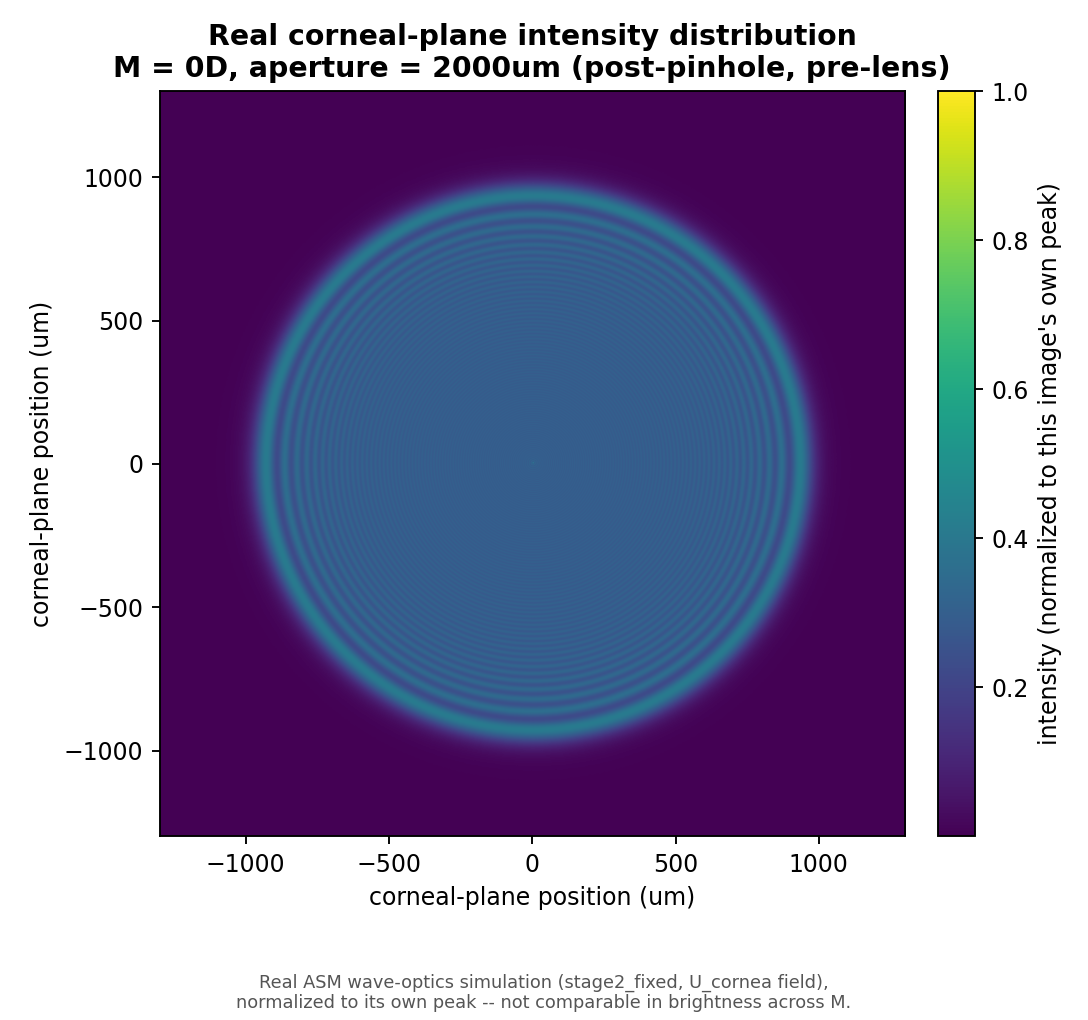
\includegraphics[width=\textwidth]{figures/corneal_illumination_M0.png}
\end{minipage}
\hfill
\begin{minipage}{0.48\textwidth}
\centering
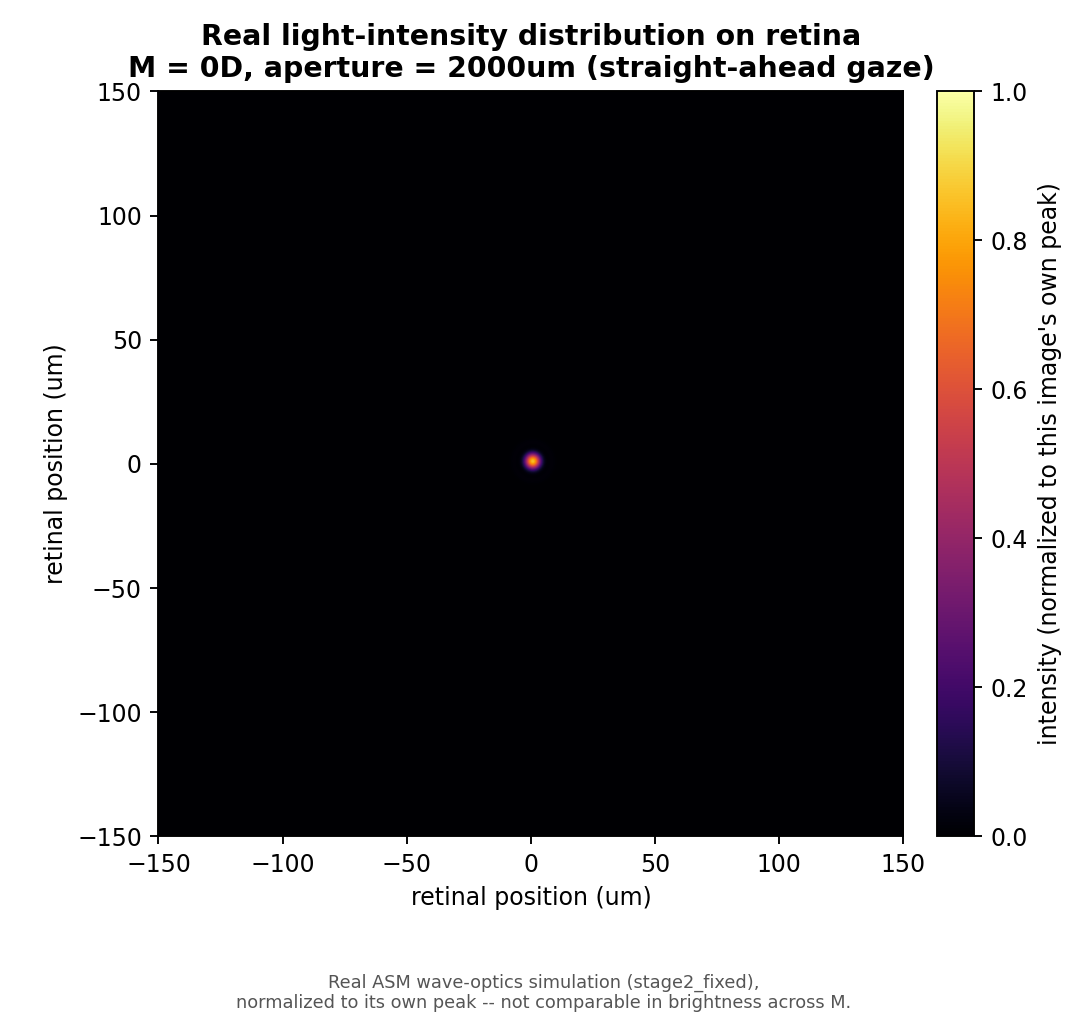
\includegraphics[width=\textwidth]{figures/realistic_heatmap_M0.png}
\end{minipage}

\vspace{6pt}
\begin{minipage}{0.48\textwidth}
\centering
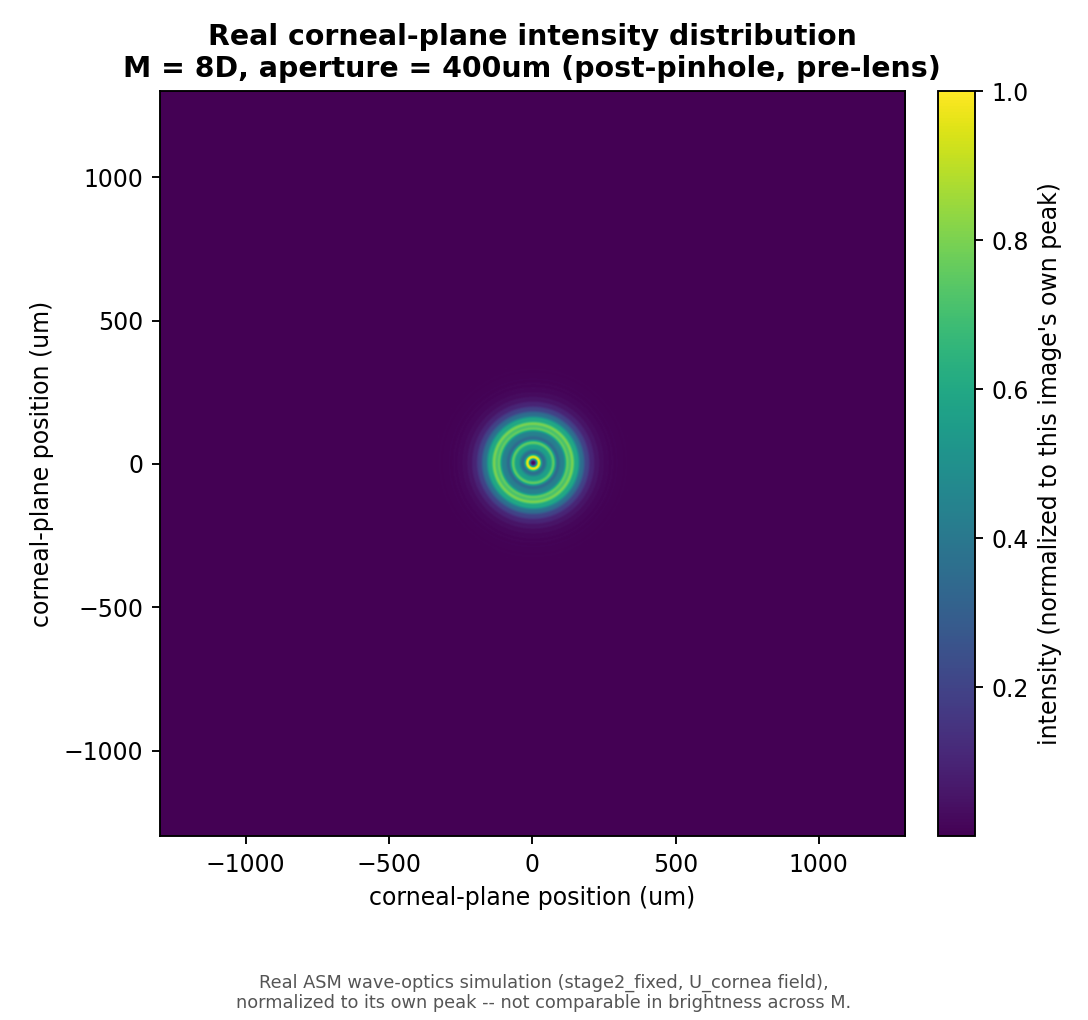
\includegraphics[width=\textwidth]{figures/corneal_illumination_M8.png}
\end{minipage}
\hfill
\begin{minipage}{0.48\textwidth}
\centering
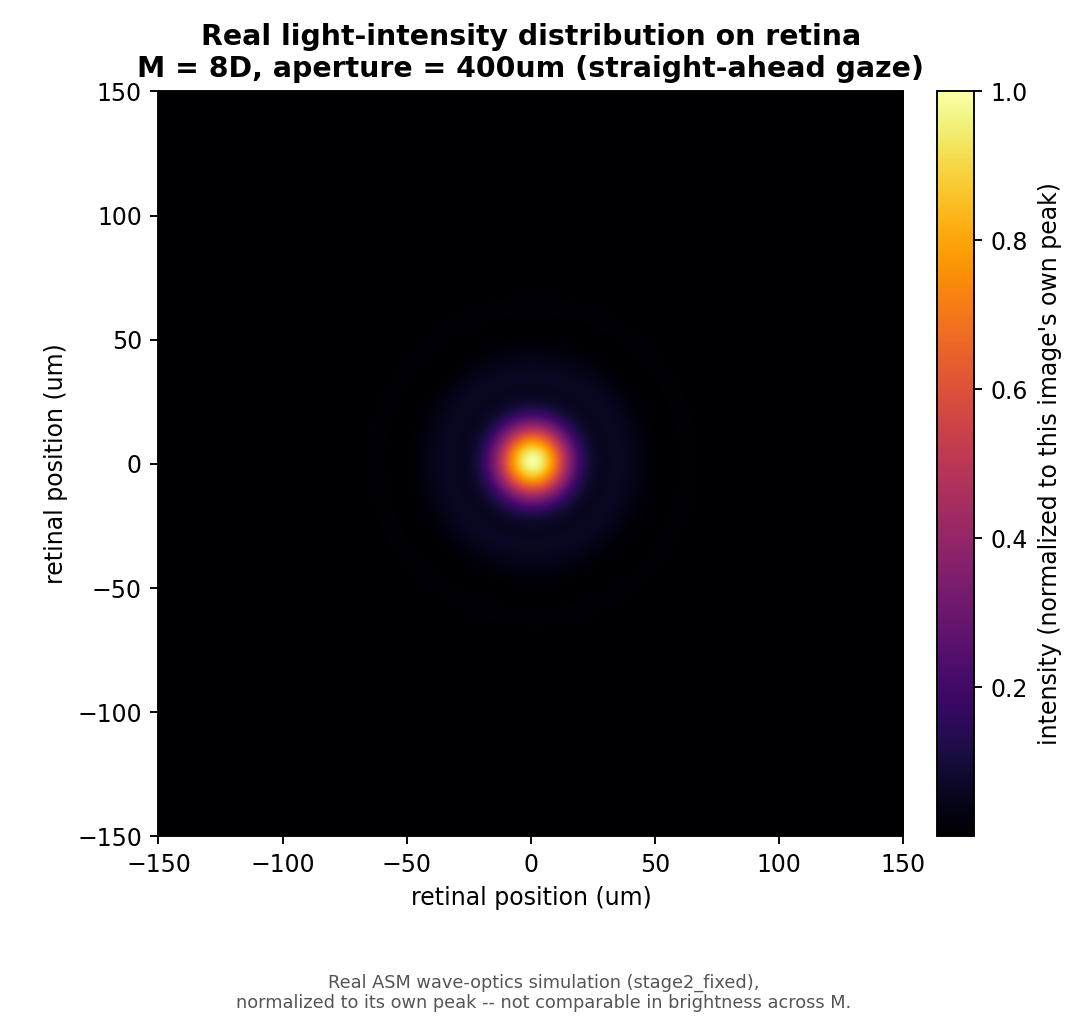
\includegraphics[width=\textwidth]{figures/realistic_heatmap_M8.png}
\end{minipage}
\caption{The pipeline chain made concrete: real $|U|^2$ intensity at the corneal
plane (left column, step~1 of the chain above, post-pinhole/pre-lens) versus the
real retinal intensity after the full lens-phase and myopic-axial-distance
propagation (right column, step~5). Top row $M=0$D, $a_{\mathrm{hole}}=2000\,\mu$m;
bottom row $M=8$D, $a_{\mathrm{hole}}=400\,\mu$m -- the two extremes of the real
per-$M$ aperture map (\texttt{array\_data/evaluation\_results/}
\texttt{PRIMARY\_WINNER\_PER\_M.csv}, mtime 2026-09-13 14:10). The corneal-plane
panels show genuine near-field Fresnel ringing at the aperture edge -- the field
has propagated only $d_{\mathrm{gap}}=12$\,mm and still closely resembles the
aperture's own geometric shape; the retinal panels show the same energy after the
myopic axial propagation, now dominated by defocus blur rather than the aperture's
edge structure. Both column pairs generated by the same
\texttt{run\_pipeline\_point()} call (one call yields both fields; no extra
propagation was run to make this comparison) --
\texttt{figure\_scripts/build\_corneal\_illumination.py} (this paper, new) and
\texttt{Array\_Design/array\_geometry\_lab/retinal\_light\_distribution\_simulation/}
\texttt{realistic\_heatmaps/build\_realistic\_heatmaps.py} (mtime of its outputs:
2026-09-28 11:15--11:16). Each panel normalized to its own peak -- absolute
brightness is not comparable across panels without a source-power calibration this
project has not made (Section~\ref{sec:limitations-optics}).}
\label{fig:cornea-vs-retina}
\end{figure}

\subsection{The effective-wavelength correction}
\label{sec:wavelength-correction}
The lens phase screen and the retina-propagation step must use the \emph{same}
effective wavelength -- $\lambda_{\mathrm{eff}}=\lambda/n'$ when
\texttt{refractive\_index\_correction=True} (this project's default), else the raw
vacuum wavelength $\lambda$. This effective wavelength is resolved \emph{once}, in
\texttt{run\_pipeline\_point}, and threaded through both the lens-phase and
retina-propagation calls -- a design choice made specifically because an earlier
version of this project's code did not do this (Section~\ref{sec:bug-fft}, the
single-FFT defocus-plane bug and its root cause both trace to exactly this
wavelength-consistency issue).

\section{Fresnel number: which diffraction regime a given stage is in}
\label{sec:fresnel-number}
\begin{equation}
N_F = \frac{R_{\mathrm{hole}}^2}{\lambda z}
\end{equation}
$N_F \ll 1$ corresponds to the far field (a clean Airy pattern); $N_F \sim 1$--$10$ is
the Fresnel transition regime (several comparably-bright diffraction rings); $N_F \gg
10$ is near-geometric (a sharp-edged projected patch, diffraction a small correction).
This project's own sweeps span Fresnel numbers well under 1 to over 20 across the
full aperture$\times$myopia grid (source:
\texttt{Array\_Design/array\_geometry\_lab/Physics\_Guide/MASTER\_HANDBOOK.tex} Chapter 6)
-- i.e.\ the mask-to-cornea and lens-to-retina propagation stages routinely sit in
\emph{different} regimes from each other within a single evaluated point, which is the
direct justification for using the regime-agnostic exact method (Equation~\ref{eq:asm})
rather than a regime-specific closed form for either stage.

\section{Numerical implementation: grid, band-limiting, and energy accounting}
\label{sec:numerics}
The ASM integral is evaluated on a finite square grid of $N\times N$ samples spanning a
physical window $L$ (so pixel pitch $dx=L/N$), via FFT. Two numerical issues require
explicit handling, both already present in the implementation and both logged, not
silently corrected:

\textbf{Band-limiting.} A finite grid cannot represent spatial frequencies beyond its
own Nyquist limit; a hard-edged pinhole mask has high-frequency content that, left
unfiltered, aliases into spurious fine structure that is numerically indistinguishable
from genuine diffraction structure. The Matsushima band limit \citep{matsushima2009} suppresses spectral
content beyond the angle at which this aliasing would occur; every run logs the
suppressed energy fraction explicitly, rather than treating it as an unaccounted loss.

\begin{keybox}{Why the energy-conservation check itself needed correcting}
Since the propagation kernel $H$ in Equation~\ref{eq:asm} has unit modulus on every
retained (propagating) spectral component and is exactly zero on every suppressed
(evanescent or band-limited) one, the apparent energy loss after propagation is
\emph{identically} the band-limit-suppressed spectral fraction:
$\varepsilon_{\mathrm{energy}} \equiv f_{\mathrm{suppressed}}$ -- confirmed against this
project's own sweep data at correlation $1.000000$ (source: \texttt{MASTER\_HANDBOOK.tex}
Chapter 6, ``Numerical band-limiting''). An energy-conservation test written against a
flat tolerance (``energy in must equal energy out to within $\epsilon$'') would
therefore fail on \emph{every single row} from this intentional, already-accounted-for
suppression alone, never distinguishing it from a genuine bug. The corrected test
instead checks the \emph{residual}
$\varepsilon_{\mathrm{energy}} - f_{\mathrm{suppressed}}$, which is near zero when the
implementation is correct and would flag a real discrepancy if one existed -- restoring
the check's actual diagnostic power.
\end{keybox}

\section{Grid-resolution artifact and the grid$\_N$ fix}
\label{sec:gridN}
A specific, separate numerical defect was found and fixed during this project's own
development, independent of the physics above: the ASM propagation grid resolution
$N_{\mathrm{grid}}$ defaults to $2048$ in
\texttt{stage4\_human\_vision/pipeline.py}'s \texttt{run\_stage4\_point} function
(verified: line \texttt{grid\_N=2048} in the function signature, current file). At this
resolution, computed blur radii for \emph{large} apertures ($\gtrsim1500$--$2000\,\mu$m)
come out approximately \textbf{2$\times$ too large} compared to the converged value at
$N_{\mathrm{grid}}=4096$ -- a genuine numerical under-resolution artifact, not a
physical effect. \texttt{new\_sweeps/run\_blur\_sweep.py} was corrected to pass
$N_{\mathrm{grid}}=4096$ explicitly on 2026-08-16; the acuity-model sweep script,
\texttt{new\_sweeps/run\_acuity\_sweep.py}, called the same underlying function but was
\emph{not} updated to match until 2026-09-12/13, leaving every acuity-model number
computed from that script stale for nearly a month. This specific staleness episode,
its full blast-radius accounting, and its remediation are documented as a worked case
study in Section~\ref{sec:bug-gridN}.

\section{Validation of the ASM engine}
\label{sec:asm-validation}
At the closed-form-tractable limit ($d_{\mathrm{gap}}\to0$, $M=0$), the pipeline output
was checked directly against the exact Fraunhofer diffraction result for a circular
aperture:
\begin{equation}
I(r) = I_0\left(\frac{2J_1(x)}{x}\right)^2, \qquad x = \frac{\pi a r}{\lambda v_r},
\qquad
EE(x) = 1 - J_0^2(x) - J_1^2(x)
\end{equation}
Agreement is within 2\% on the 50\%- and 90\%-encircled-energy radii. The 80\%-radius
check needs 8\% tolerance: the first Airy-pattern null sits at $x=3.8317$, where
$EE\approx0.838$ -- almost exactly the 80\% level, on a flat part of the encircled-energy
curve where a small energy error maps to a disproportionately large radius error.
Repeating the check at grid sizes from 1024 through 8192 never brought this residual
below 2.3--4.6\%, confirming it is genuine ill-conditioning of that specific percentile
at that specific aperture regime, not an under-resolved grid (source:
\texttt{MASTER\_HANDBOOK.tex} Chapter 6, ``Validation against the closed form'').

Separately, the on-axis intensity was checked against the closed-form Fresnel-zone
oscillation $I(0,z)=4I_0\sin^2(\pi N_F/2)$ and matched at correlation $0.997$ -- direct
confirmation that the non-monotonic Strehl-ratio behaviour this project's sweeps show
(multiple local maxima as aperture is swept at fixed $M$) is real Fresnel-zone
interference, not numerical noise, and is one of the reasons the RSS model
(Section~\ref{sec:rss}), which is smooth and monotonic by construction, cannot
represent this project's own actual blur behaviour.

\section{Blur metrics and where each one breaks}
\label{sec:blur-metrics}
\begin{center}
\begin{tabular}{p{2.6cm}p{4.8cm}p{6.0cm}}
\toprule
Metric & Measures & Failure mode \\
\midrule
$r_{EE}(50\%)$ & Radius enclosing half the retinal energy & Stable and monotonic in
aperture, but overestimates clinical acuity loss by roughly $7\times$ against measured
clinical data (Chapter~\ref{ch:model-comparison}) \\
FWHM & Width of the central diffraction/blur core only & Tracks clinical acuity loss
more closely ($\sim1.6\times$) but is \emph{discontinuous} in the design variable: a
jump from $4.7\,\mu$m to $154.7\,\mu$m was observed between two apertures only
$250\,\mu$m apart at $M=4$D, from ring-hopping between local intensity maxima \\
Strehl ratio & Peak intensity relative to the diffraction limit & Genuinely
multi-peaked (6--7 local maxima across the aperture sweep at fixed $M$), confirmed
\emph{worse} (more, not fewer, peaks resolved), not numerically better, at $10\times$
finer grid sampling -- i.e.\ this is real physics (matched to the Fresnel-zone
closed form above), not numerical noise to be smoothed away \\
\bottomrule
\end{tabular}
\end{center}

\begin{keybox}{Why $r_{EE}(50\%)$ is used as the project's standard optimization metric anyway}
Per individual aperture, FWHM is unusable as an optimization target because it is
discontinuous in the very variable being optimized. Across a coarse sweep its
\emph{trend} tracks clinical reality more closely than $r_{EE}(50\%)$, which is smooth
and numerically well-behaved but systematically pessimistic by roughly $7\times$. This
project reports $r_{EE}(50\%)$ as its blur-optimization metric throughout and states its
known bias explicitly, rather than optimizing against a metric that is discontinuous in
the design variable it is meant to optimize.
\end{keybox}

\section{Deprecated formulas}
\label{sec:deprecated}
\begin{center}
\begin{tabular}{p{5.4cm}p{7.4cm}}
\toprule
Formula & Status and measured error \\
\midrule
$r_{\mathrm{geo}} = \dfrac{a_{\mathrm{hole}}}{2}\dfrac{|v_r-v_f|}{v_f}$ & Deprecated.
Superseded by the direct ASM chain (Section~\ref{sec:asm}), which produces this effect
automatically without a separate geometric-blur term. \\
$r_{\mathrm{tot}}=\sqrt{r_{\mathrm{geo}}^2+r_{\mathrm{diff}}^2}$ (RSS,
Section~\ref{sec:rss}) & Deprecated. 64.8\% mean, 192.8\% maximum divergence from the
exact result. \\
$a_{\mathrm{eff}}\approx\sqrt{a_{\mathrm{hole}}^2+(2.44\lambda d_{\mathrm{gap}}/a_{\mathrm{hole}})^2}$
& Deprecated. Smooth and monotonic by construction; cannot represent the genuine
Fresnel-zone oscillation confirmed in Section~\ref{sec:asm-validation}. \\
\bottomrule
\end{tabular}
\end{center}

\section{Array optics reuse single-aperture optics unmodified}
\label{sec:array-vs-single}
Every hole in a fabricated array has optics \emph{identical} to a standalone single
aperture of the same diameter $a_{\mathrm{hole}}$ at the same myopia power $M$: the
array geometry changes only whether zero, one, or multiple holes' images
simultaneously reach the retina (blinding, clean imaging, or ghosting -- Chapter
\ref{ch:array-theory}), never the per-hole blur itself. This is why every array
evaluation result in this paper (Chapters~\ref{ch:model-a}--\ref{ch:model-b}) looks up
its predicted acuity directly from the single-aperture sweep at the array's own chosen
aperture, rather than re-deriving acuity per array family -- a claim independently
confirmed in this paper's own analysis (Section~\ref{sec:model-comparison-table}): all
six array evaluation models tested produce numerically identical predicted LogMAR per
myopia power, differing only in which \emph{geometry} carries that identical optical
aperture.

\chapter{The Acuity Model}
\label{ch:acuity}

A blur radius alone is not the quantity a clinician, or an IYPT judge, ultimately cares
about: the relevant output is predicted \emph{visual acuity}, conventionally reported
in LogMAR (log Minimum Angle of Resolution) or Snellen notation. This project converts
the ASM-computed retinal blur into a LogMAR prediction via a specific, cited pipeline
implemented in \texttt{stage4\_human\_vision/acuity.py} (verified read directly).

\section{Why blur radius is the wrong optimization target on its own}
Minimizing a blur-radius metric directly (e.g.\ $r_{EE}(50\%)$) does not necessarily
minimize predicted acuity loss, because the mapping from blur to acuity is nonlinear and
itself depends on the eye's own optical transfer function and on retinal illuminance,
not on blur radius alone. \texttt{MASTER\_HANDBOOK.tex} Chapter~5 documents two
successive corrections made to an earlier, blur-radius-only optimization approach: first
an explicit brightness floor (Section~\ref{sec:brightness}), then optimizing acuity
directly rather than blur (used throughout this project's array-evaluation chapters).

\section{Pupil and retinal illuminance}
Retinal illuminance is computed from the light entering through the active aperture(s)
at a given gaze condition, scaled by scene luminance, and reported in trolands (Td),
the standard unit for retinal illuminance referenced to pupil area. This project's
default scene luminance is $10{,}000\,\mathrm{cd/m^2}$ (bright outdoor daylight), with
default field diameter $20^\circ$ and default observer age $28.58$ years (source:
\texttt{stage4\_human\_vision/config.py} defaults, \texttt{default\_scene\_luminance\_cdm2},
\texttt{default\_field\_diameter\_deg}, \texttt{default\_age\_years}; verified present).

\section{MTF, contrast sensitivity, and Visual Strehl}
The acuity predictor uses the aperture's actual modulation transfer function (MTF,
derived from the ASM-computed point spread function), evaluated against a contrast
sensitivity function (CSF) model, and a Visual Strehl ratio (VSOTF) -- the CSF-weighted
similarity of the actual optical transfer function to the diffraction-limited one --
as an overall optical-quality summary statistic. This is the same VSOTF/CSF machinery
discussed in detail, with a documented correction, in the array-level ghosting theory
(Section~\ref{sec:barten}); the acuity model here uses \texttt{stage3\_human\_vision}'s
own optical-quality and CSF evaluation directly, not a re-implementation.

\subsection{The recommended predictor}
\begin{align}
\mathrm{MAR}_{10} &= \frac{f_{20/20}}{f_{\mathrm{cutoff,10\%}}}
& \text{(MAR from the MTF's 10\% cutoff spatial frequency)} \\
\mathrm{MAR}_{\mathrm{VSOTF}} &= \frac{\mathrm{MAR}_{10}}{\mathrm{clip}(\mathrm{VSOTF},0.25,2.0)^{0.1}}
& \text{(Visual-Strehl adjustment)} \\
\mathrm{LogMAR}_{\mathrm{raw}} &= \log_{10}\!\big(\max(\mathrm{MAR}_{\mathrm{VSOTF}},10^{-6})\big)
\end{align}
This is the \texttt{mtf10\_vsotf\_brightness\_adjusted} model (source:
\texttt{stage4\_human\_vision/acuity.py}, function \texttt{predict\_acuity}, verified
read directly), the ``recommended'' model this project selects by configuration, not
chosen post-hoc per result.

A legacy alternative predictor (an uncited $\mathrm{SNR}^{0.05}$ correction term, in the
same file, function argument \texttt{legacy\_mar}) is retained in the codebase for
direct comparison, per this project's own stated design principle of keeping
alternative models available rather than silently deleting a superseded one
(\texttt{DESIGN.md}, cited in \texttt{acuity.py}'s own module docstring).

\begin{figure}[htbp]
\centering
\begin{minipage}{0.23\textwidth}\centering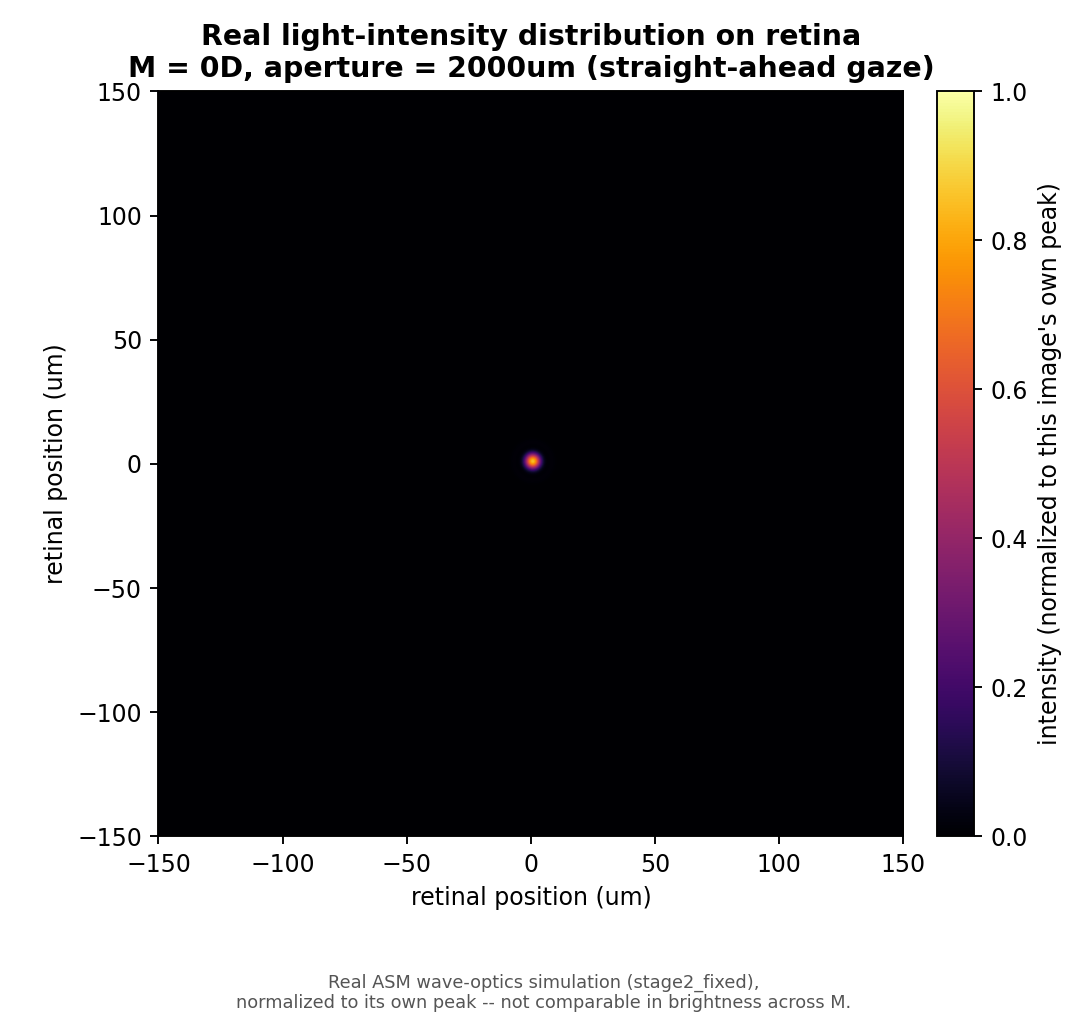
\includegraphics[width=\textwidth]{figures/realistic_heatmap_M0.png}\end{minipage}
\begin{minipage}{0.23\textwidth}\centering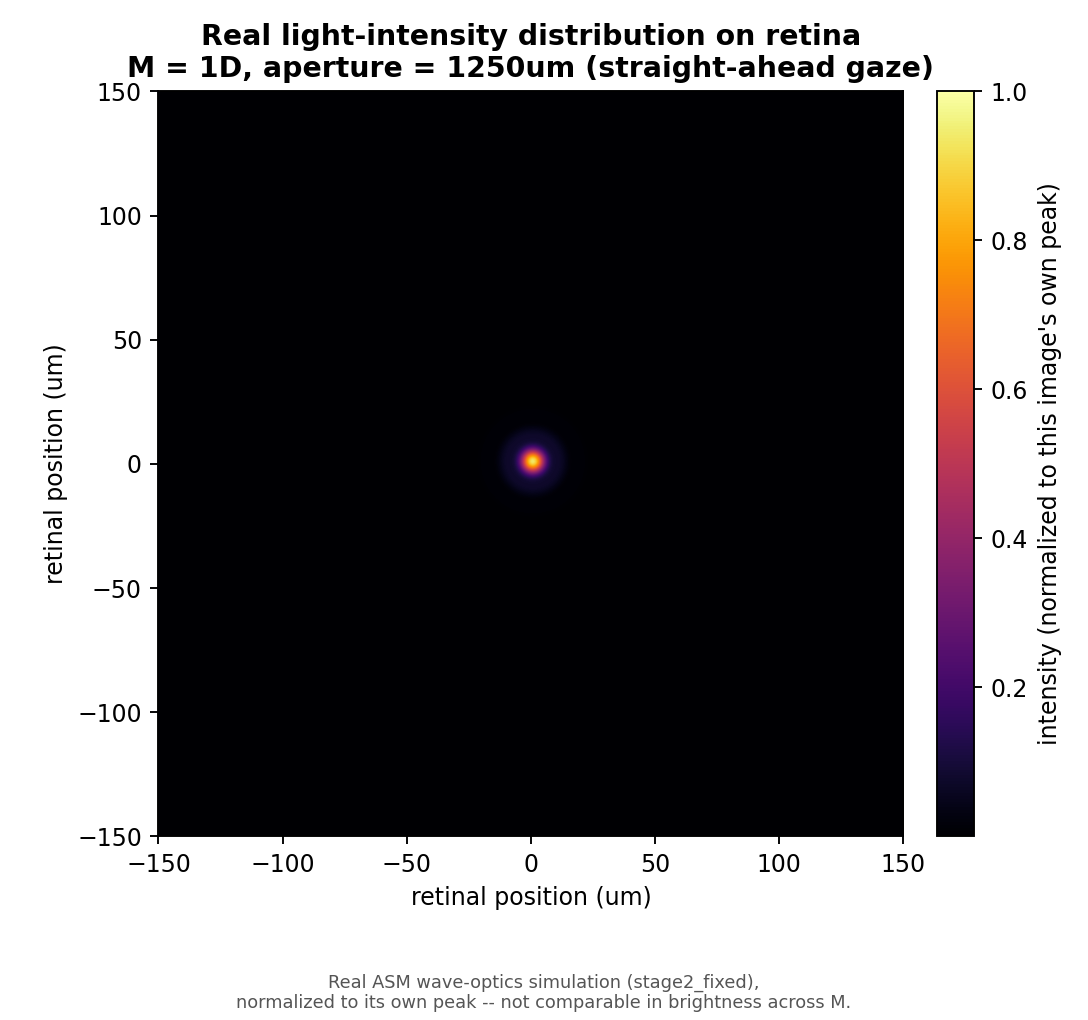
\includegraphics[width=\textwidth]{figures/realistic_heatmap_M1.png}\end{minipage}
\begin{minipage}{0.23\textwidth}\centering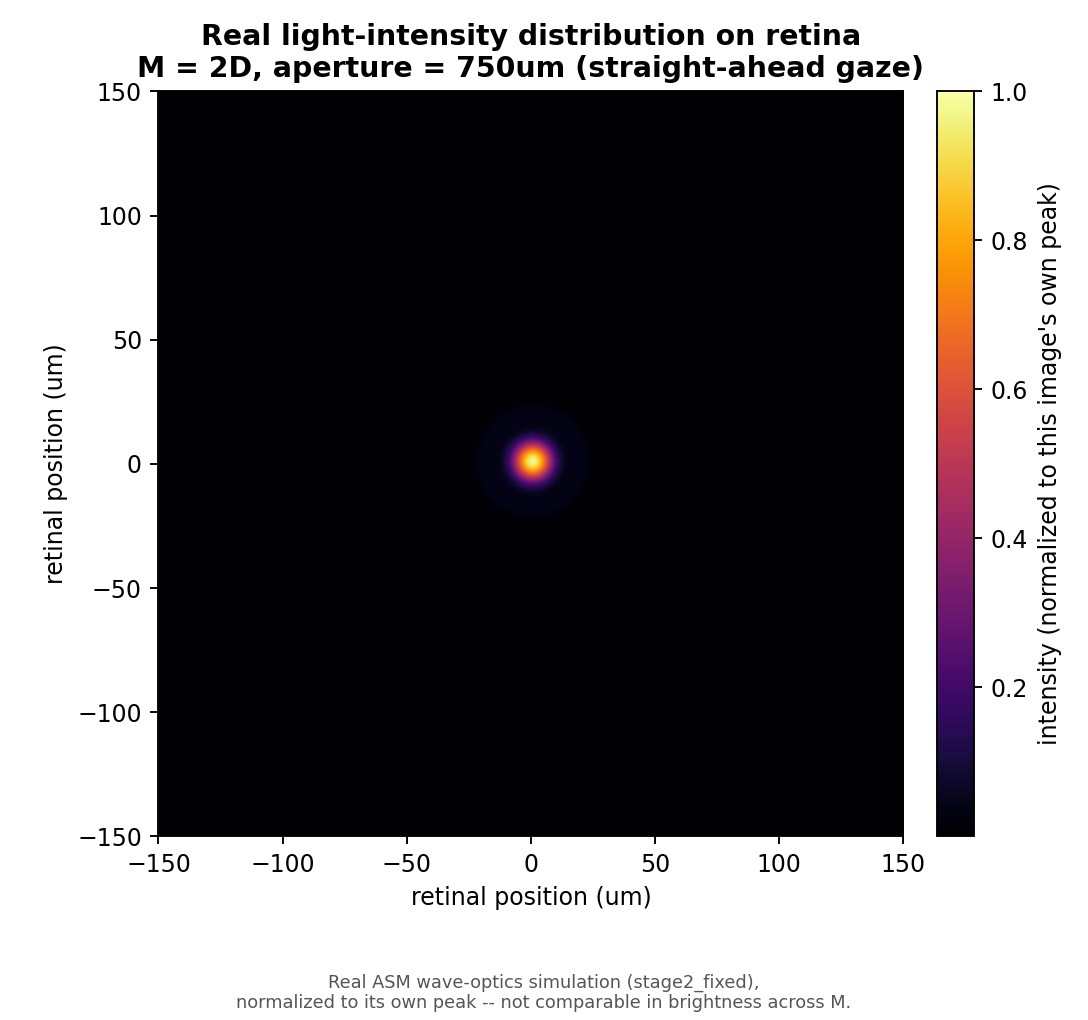
\includegraphics[width=\textwidth]{figures/realistic_heatmap_M2.png}\end{minipage}
\begin{minipage}{0.23\textwidth}\centering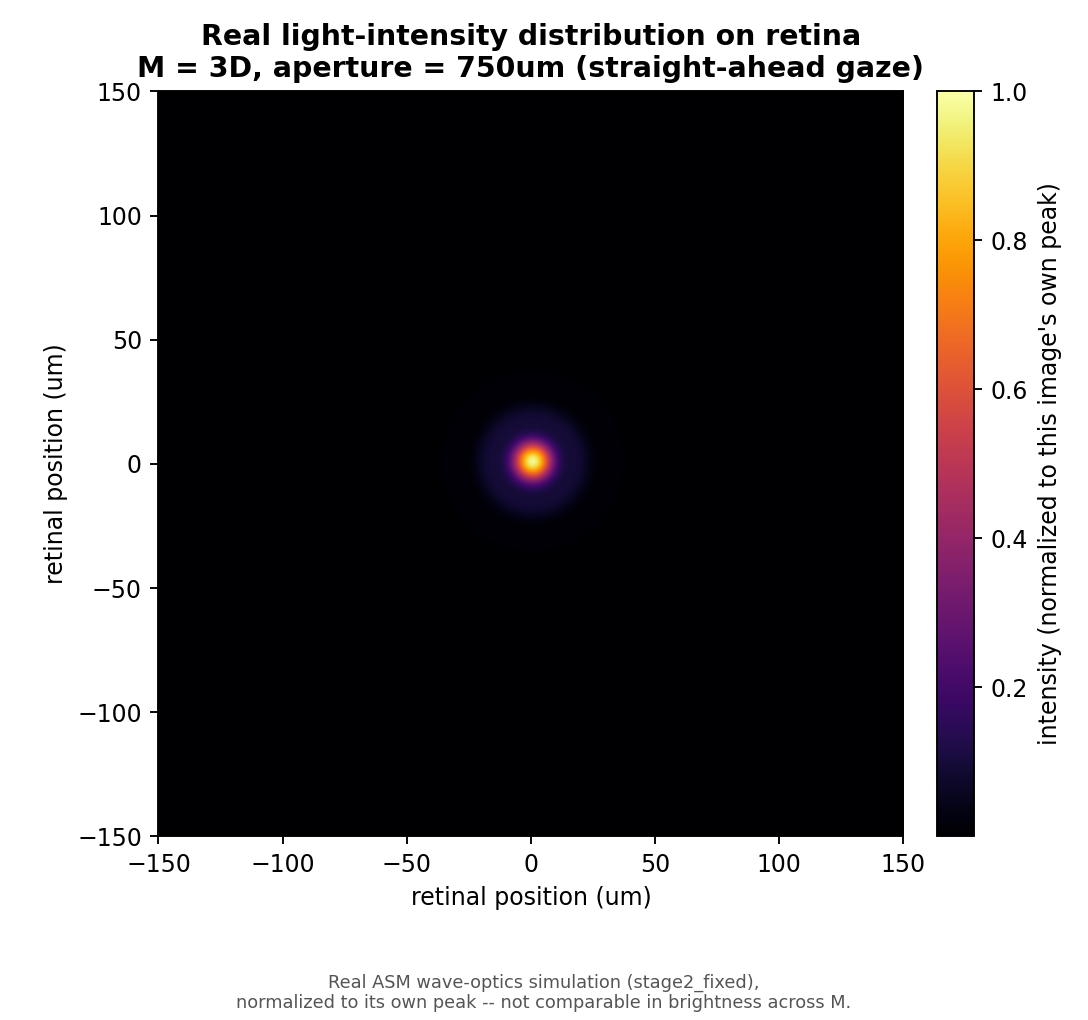
\includegraphics[width=\textwidth]{figures/realistic_heatmap_M3.png}\end{minipage}

\vspace{4pt}
\begin{minipage}{0.23\textwidth}\centering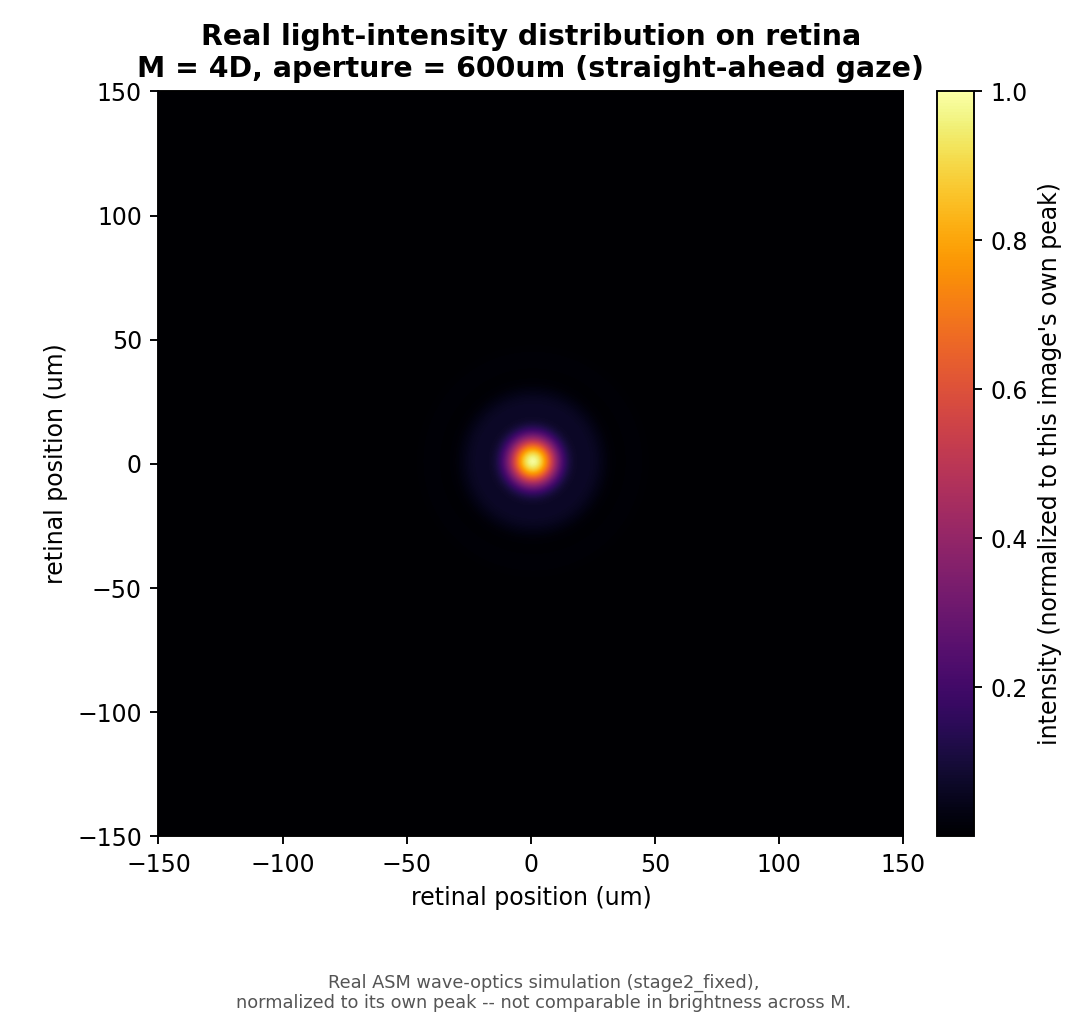
\includegraphics[width=\textwidth]{figures/realistic_heatmap_M4.png}\end{minipage}
\begin{minipage}{0.23\textwidth}\centering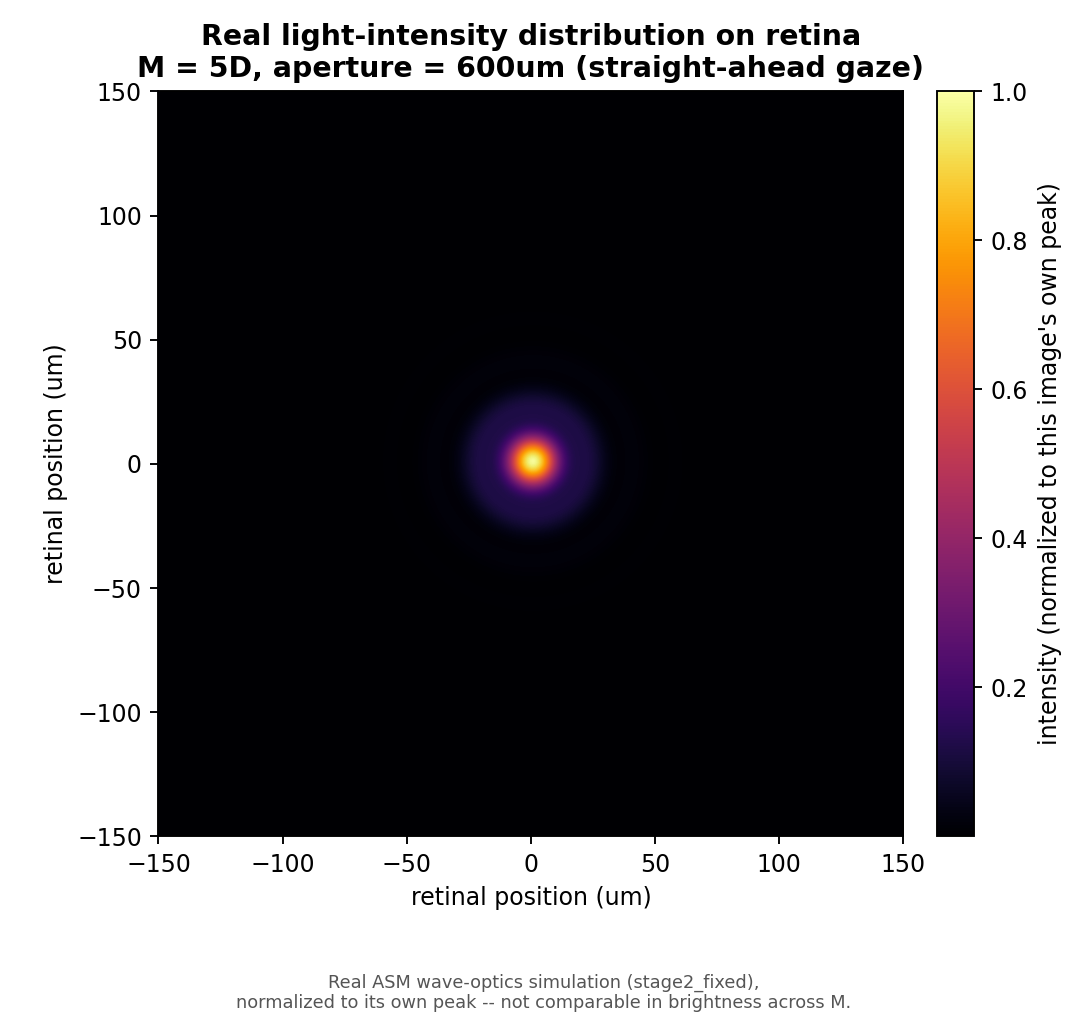
\includegraphics[width=\textwidth]{figures/realistic_heatmap_M5.png}\end{minipage}
\begin{minipage}{0.23\textwidth}\centering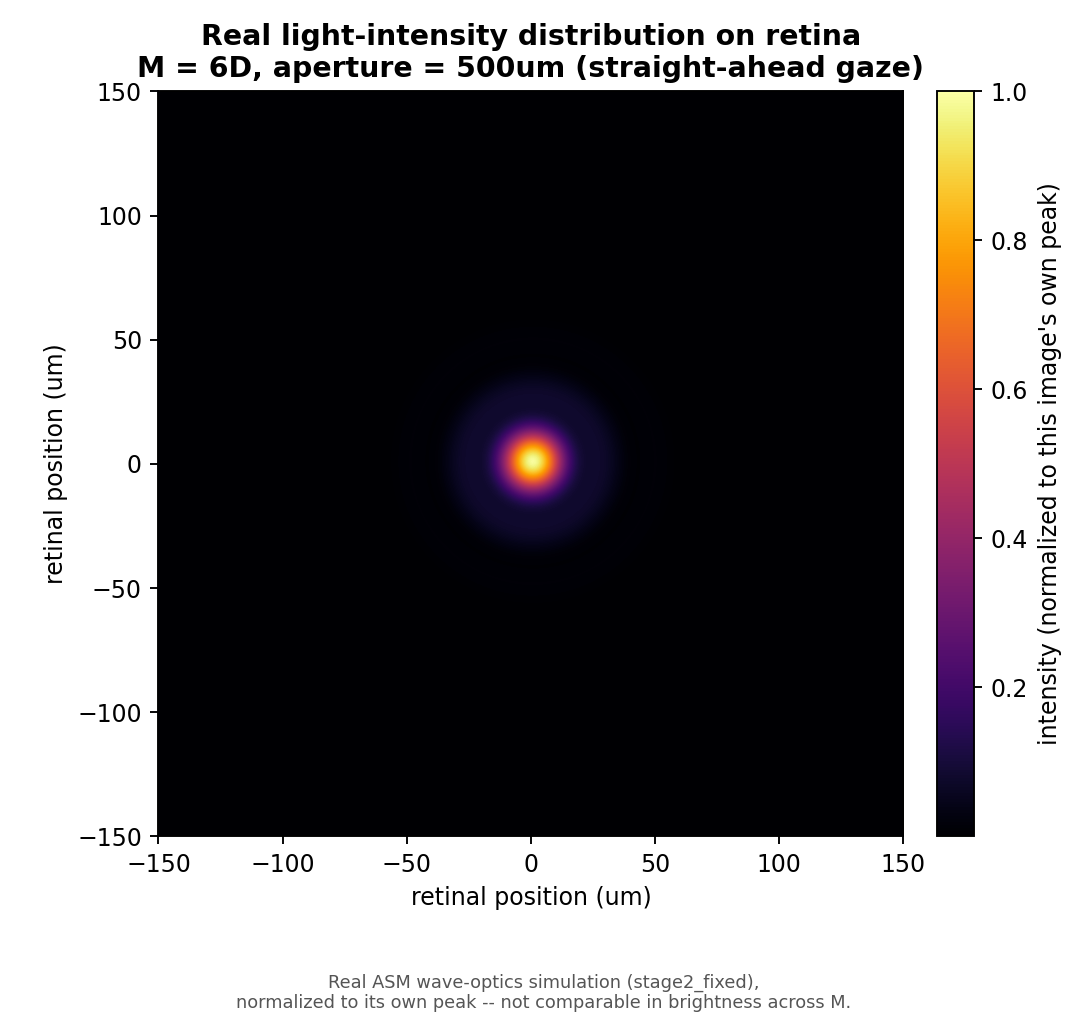
\includegraphics[width=\textwidth]{figures/realistic_heatmap_M6.png}\end{minipage}
\begin{minipage}{0.23\textwidth}\centering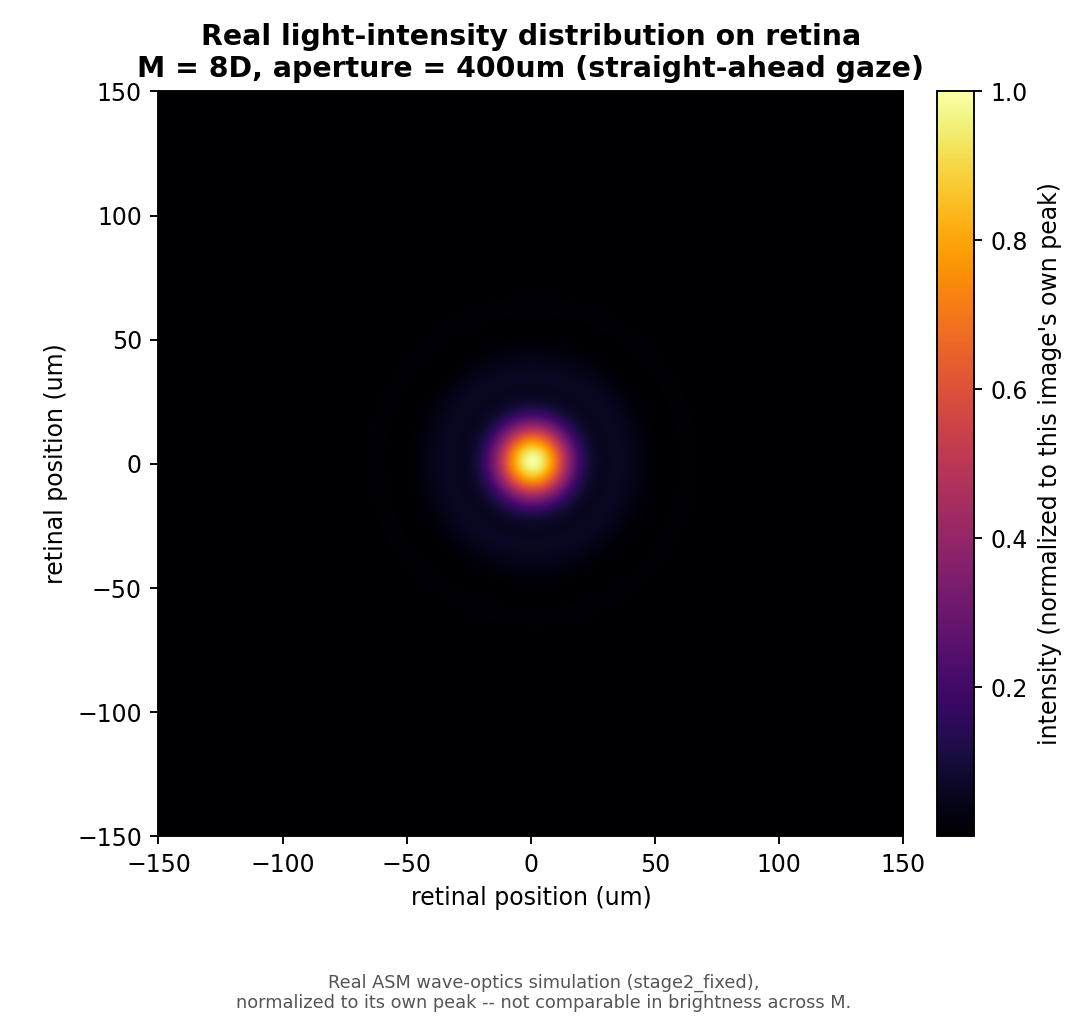
\includegraphics[width=\textwidth]{figures/realistic_heatmap_M8.png}\end{minipage}
\caption{Real retinal-plane intensity ($I_{\mathrm{retina}}=|U_{\mathrm{retina}}|^2$,
straight-ahead gaze) for all eight modeled myopia powers, left to right:
$M=0,1,2,3$D (top row), $M=4,5,6,8$D (bottom row), each at that $M$'s real
\texttt{PRIMARY\_WINNER\_PER\_M.csv} aperture. Every panel is the actual ASM
wave-optics output, not a schematic -- the growing blur radius from $M{=}0$ to
$M{=}8$ visible here is the same physical quantity the LogMAR curve above is
predicting a number for. Source:
\texttt{Array\_Design/array\_geometry\_lab/retinal\_light\_distribution\_simulation/}
\texttt{realistic\_heatmaps/realistic\_heatmap\_M\{0,1,2,3,4,5,6,8\}.png}, all eight
generated 2026-09-28 11:15--11:16 (verified via \texttt{stat}); each panel
normalized to its own peak, not comparable in absolute brightness across $M$
(Section~\ref{sec:limitations-optics}).}
\label{fig:retinal-grid-all-M}
\end{figure}

\section{The brightness correction}
\label{sec:brightness}
An additive LogMAR penalty is applied in the log domain for retinal illuminance below a
literature-cited knee:
\begin{equation}
\Delta\mathrm{LogMAR}_{\mathrm{brightness}} =
\begin{cases}
0 & E_{\mathrm{td}} \ge E_{\mathrm{knee}} \\[4pt]
s \cdot \log_{10}\!\left(\dfrac{E_{\mathrm{knee}}}{E_{\mathrm{td}}}\right) &
E_{\mathrm{td}} < E_{\mathrm{knee}}
\end{cases}
\label{eq:brightness}
\end{equation}
with knee $E_{\mathrm{knee}}=300$\,Td and slope $s=0.060$ LogMAR per log$_{10}$-unit of
illuminance (source: \texttt{stage4\_human\_vision/acuity.py},
\texttt{brightness\_logmar\_correction}, verified read directly).

\textbf{Knee value (300\,Td)}: cited to Van Nes \& Bouman (1967) \citep{vannes1967} --
threshold modulation (contrast sensitivity) is illuminance-\emph{independent}
(Weber--Fechner behaviour) above 300\,Td, and increases as $E_{\mathrm{td}}^{-1/2}$
(de~Vries--Rose behaviour) below it. Verified directly against the primary abstract per
this project's own citation-verification discipline (\texttt{stage4\_human\_vision/literature.py}).

\textbf{Slope (0.060 LogMAR/log$_{10}$-unit)}: cited to Tidbury, Czanner \& Newsham
(2016), verified directly against the full text (their Table 3, $p<0.001$), and
cross-checked (not directly used) against Sheedy, Bailey \& Raasch (1984)'s
independently-derived value of $\approx0.0664$, which could only be verified against a
secondary summary rather than the primary source -- the directly-verified Tidbury value
is the one used, per this project's stated preference for primary-source-verified
citations over secondary ones of comparable magnitude.

Rabin (1994) is cited as independent corroboration of the qualitative direction of this
effect (visual acuity is considerably \emph{more} resistant to reduced luminance than
contrast sensitivity is, in the photopic range they tested: a $116\to0.23\,\mathrm{cd/m^2}$
reduction gave a $3\times$ acuity loss against a $17\times$ contrast-sensitivity loss)
-- but the exact numerical knee and slope used in Equation~\ref{eq:brightness} come from
Van Nes \& Bouman and Tidbury et al.\ respectively, both natively reported in the units
this equation needs (trolands, LogMAR), not from Rabin's own cd/m$^2$-based data.

Every design evaluated in this project's array chapters (Chapters~\ref{ch:model-a},
\ref{ch:model-b}) sits well above the 300\,Td knee at the default $10{,}000\,\mathrm{cd/m^2}$
scene luminance; the brightness term is therefore \textbf{inert (zero)} for every
reported result in this paper, and is documented here in full for completeness and
falsifiability, not because it changes any headline number.

\section{Full acuity-model input inventory}
\begin{center}
\begin{tabular}{lll}
\toprule
Input & Default value & Source \\
\midrule
Scene luminance & $10{,}000\,\mathrm{cd/m^2}$ & \texttt{config.py} \\
Field diameter & $20^\circ$ & \texttt{config.py} \\
Observer age & $28.58$ years & \texttt{config.py} \\
Pupil diameter & $4000\,\mu$m & project-wide constant \\
ASM grid resolution & $4096$ (post-fix, Section~\ref{sec:gridN}) & \texttt{run\_acuity\_sweep.py} \\
Wavelength & 550\,nm (vacuum) & \texttt{run\_acuity\_sweep.py} \\
Spectacle gap & 12\,mm & \texttt{run\_acuity\_sweep.py} \\
\bottomrule
\end{tabular}
\end{center}

\chapter{Single-Aperture Experimental Validation}
\label{ch:single-exp}

Three independent single-aperture experimental programmes were run against the theory
of Chapter~\ref{ch:single}: a photographic scenery test scored by a no-reference image
quality metric (BRISQUE), an optical-bench defocus sweep using a frosted projection
screen, and a LogMAR acuity chart protocol. All raw data referenced below is read
directly from its own CSV; no number in this chapter is retyped from a prior summary.

\section{BRISQUE scenery test}
\label{sec:brisque}
Fifty raw DNG photographs were captured of the same outdoor scene through seven
conditions: six pinhole apertures (400, 500, 700, 1000, 1200, 1400\,$\mu$m) and one
no-pinhole (``M1-8'') control, converted to 8-bit TIFF via percentile-stretch (never
JPEG, whose tone-curve compression would clip dynamic range before measurement) and
scored with OpenCV's BRISQUE implementation (\texttt{cv2.quality.QualityBRISQUE\_compute}),
a no-reference natural-image-statistics quality metric where \emph{lower} scores
indicate a more natural-looking (less distorted) image.

\begin{center}
\begin{tabular}{lc}
\toprule
Condition & Mean BRISQUE score \\
\midrule
No-pinhole control & 39.5 \\
700\,$\mu$m & 54.9 \\
1000\,$\mu$m & 63.8 \\
1200\,$\mu$m & 67.9 \\
500\,$\mu$m & 68.5 \\
400\,$\mu$m & 68.3 \\
1400\,$\mu$m & 69.0 \\
\bottomrule
\end{tabular}
\end{center}
(source: \texttt{ExperimentalComparison/ExP1\_clarity\_analysis/measurements/brisque\_scores.csv},
mtime 2026-09-09; computed directly from the raw grouped means, not copied from a prior
report.)

\begin{figure}[htbp]
\centering
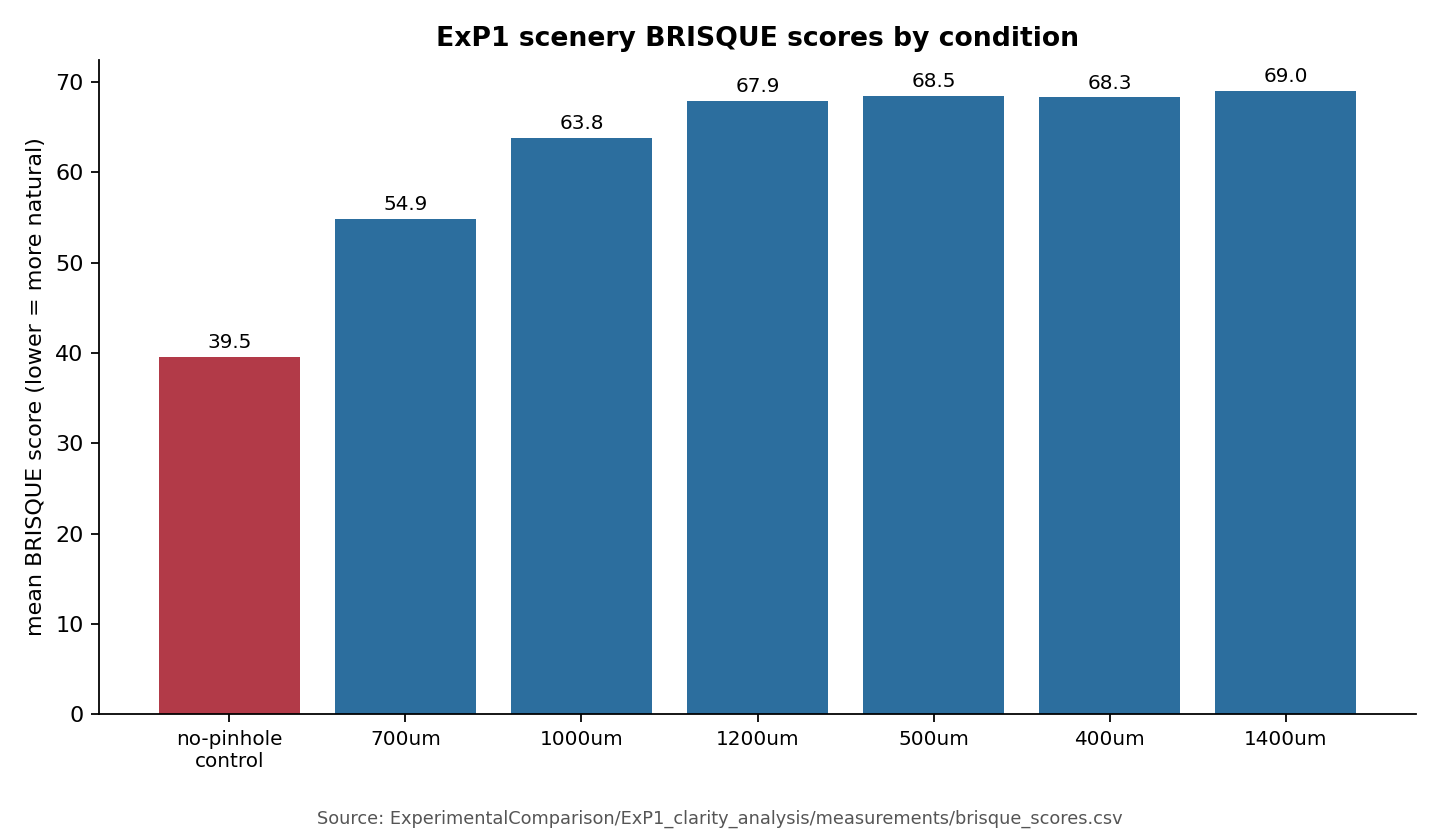
\includegraphics[width=0.85\textwidth]{figures/brisque_scenery_scores.png}
\caption{Mean BRISQUE score per condition, generated directly from the same CSV the
table above is drawn from (\texttt{ExperimentalComparison/ExP1\_clarity\_analysis/}
\texttt{measurements/brisque\_scores.csv}, mtime 2026-09-09) -- table and figure are
guaranteed consistent by construction, both computed from this one file, not
cross-checked after the fact.}
\label{fig:brisque-scenery}
\end{figure}

\begin{warnbox}{An honest, unresolved tension}
Every pinhole condition scores \emph{worse} (higher BRISQUE) than the no-pinhole
control, and scores do not monotonically improve as aperture size increases toward the
theoretical optimum -- the opposite ordering from what the blur-radius theory
(Chapter~\ref{ch:single}) predicts. BRISQUE measures general natural-image statistical
``naturalness,'' not optical sharpness directly, and a pinhole photograph -- vignetted,
lower-light, geometrically different from an unrestricted exposure -- departs from the
natural-image statistics BRISQUE was trained against for reasons that have nothing to
do with resolved blur. This is reported here exactly as found: BRISQUE is not treated in
this paper as a validated proxy for the blur-radius theory, and this discrepancy is not
smoothed over.
\end{warnbox}

\section{Frosted-screen optical-bench defocus sweep (ExP3)}
\label{sec:exp3}
A fixed pinhole (one of six apertures: 400, 500, 600, 800, 1000, 1400\,$\mu$m, plus an
unrestricted-beam control) illuminates a frosted projection screen slid along the
optical axis through five displacements (0, 5, 10, 15, 20\,mm); the illuminated spot's
radius is measured photographically at each displacement via blue-LED point-source
imaging, using BT.601 luma (\texttt{cv2.cvtColor(..., COLOR\_BGR2GRAY)}) rather than a
naive max(R,G,B) channel combination -- the correct convention for a blue-dominant
point source, confirmed during this project's own analysis.

\begin{center}
\begin{tabular}{lc}
\toprule
Condition & Growth slope (px/mm displacement) \\
\midrule
No-pinhole control (unrestricted beam) & 10.71 \\
1000\,$\mu$m & 0.88 \\
400\,$\mu$m & 0.72 \\
1400\,$\mu$m & 0.68 \\
500\,$\mu$m & 0.66 \\
800\,$\mu$m & 0.65 \\
600\,$\mu$m & 0.60 \\
\bottomrule
\end{tabular}
\end{center}
(source: \texttt{ExperimentalComparison/ExP3\_frosted\_screen/measurements/all\_spot\_measurements.csv};
slopes computed directly from a linear fit of measured spot radius against screen
displacement per condition, this analysis.)

The unrestricted-beam control's spot grows roughly \textbf{15--18$\times$ faster} with
screen displacement than any pinhole condition -- direct, controlled, photographic
confirmation of the stenopeic effect itself (Section~\ref{sec:stenopeic}): restricting
the admitted ray bundle genuinely and dramatically slows how fast defocus blur grows
with axial displacement, independent of any specific numeric optimum among the pinhole
apertures. Among the pinhole conditions themselves the slope is not perfectly monotonic
in aperture size (600\,$\mu$m measured lowest, not the largest or smallest aperture
tested) -- a real, non-monotonic experimental result, reported as measured rather than
smoothed toward the simple theoretical expectation of monotonic growth with aperture.

\begin{figure}[htbp]
\centering
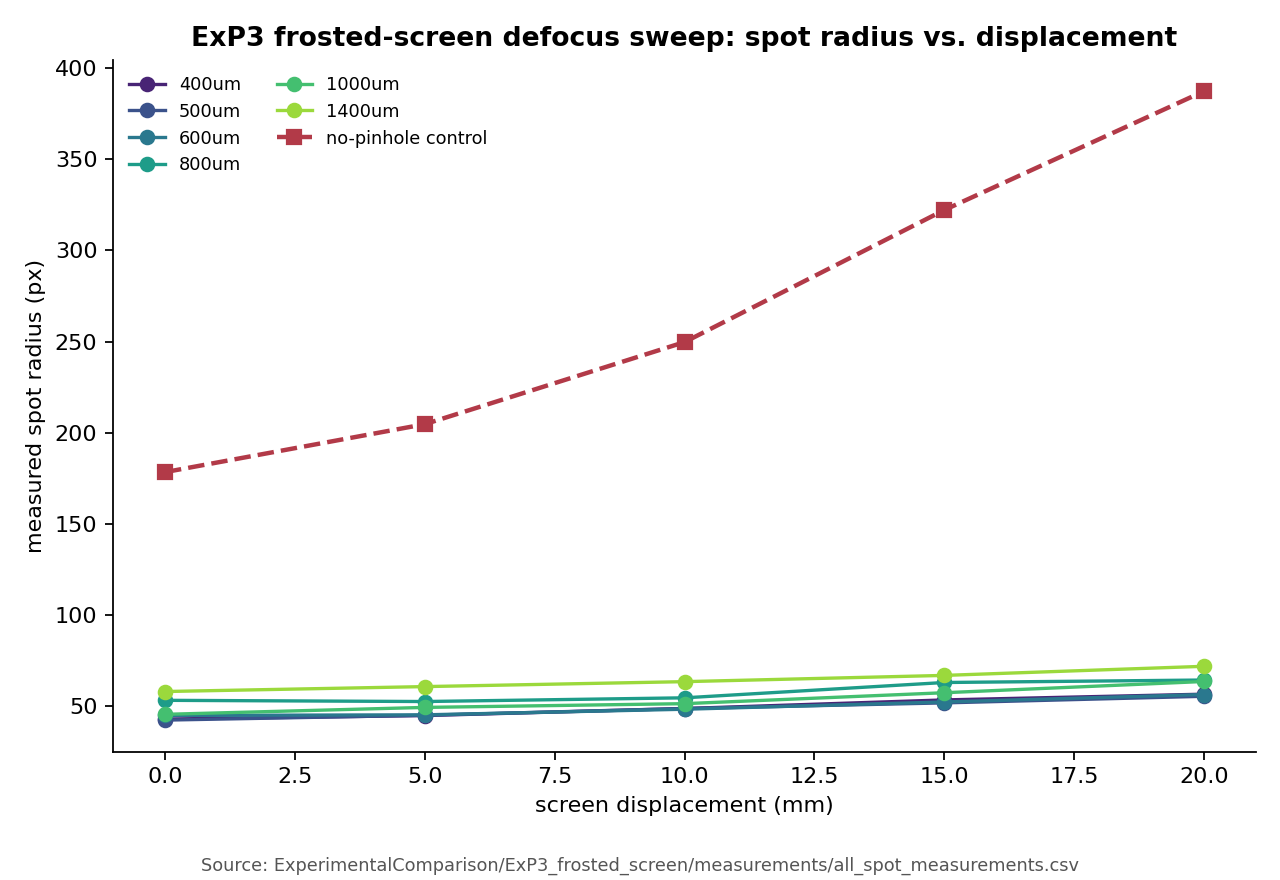
\includegraphics[width=0.85\textwidth]{figures/frosted_screen_growth_curves.png}
\caption{Measured spot radius vs.\ screen displacement, all seven conditions, from the
same CSV the growth-slope table above is fit from
(\texttt{ExperimentalComparison/ExP3\_frosted\_screen/measurements/}
\texttt{all\_spot\_measurements.csv}, mtime 2026-09-02). The no-pinhole control's much
steeper growth is directly visible, not just implied by the slope ratio in the table;
the pinhole conditions' near-overlapping, shallow curves make the non-monotonicity in
600\,$\mu$m's slope (lowest of the six, not the largest or smallest aperture) a real,
visually confirmable feature of the raw data rather than a fitting artifact.}
\label{fig:frosted-curves}
\end{figure}

\section{LogMAR acuity chart protocol}
\label{sec:logmar-protocol}
A single-pinhole logMAR acuity measurement protocol is specified in
\texttt{Array\_Design/array\_geometry\_lab/Physics\_Guide/LOGMAR\_ACUITY\_PROTOCOL.tex}
(verified present, mtime 2026-09-11): recruit subjects across a range of native myopia,
measure uncorrected acuity and pinhole-corrected acuity at a fixed viewing distance, and
compare the \emph{shape} of the resulting curve (flat vs.\ steep against myopia severity)
against the flatness prediction of Section~\ref{sec:flatness-prediction} -- a
qualitative-ranking design chosen specifically because it does not require knowledge of
any subject's exact refractive prescription, only a relative ranking of myopia severity,
and because a flat-vs-steep \emph{shape} comparison is a stronger test than comparing a
single subject to a single predicted number.

\needsverify{As of this writing, no CSV or log file recording actual executed subject
data for this protocol was found anywhere in the repository (searched: all .csv files
for a ``subject'' column or per-subject naming, all logs, all folders named with
Array-Exp/ArrayExp/clinical/trial patterns). The document above is a
\emph{protocol specification}, not a completed experiment. Section~\ref{sec:array-exp2}
addresses the array-level version of this same gap explicitly.}

\section{Reconciliation with theory}
The frosted-screen result (Section~\ref{sec:exp3}) is the cleanest, most direct
confirmation among the three single-aperture experiments: it isolates exactly the
physical quantity the stenopeic-effect argument (Section~\ref{sec:stenopeic}) predicts
-- growth rate of blur with axial defocus -- and controls for everything else (same
light source, same imaging chain, same measurement method) across every condition. The
BRISQUE result (Section~\ref{sec:brisque}) is reported honestly as \emph{not}
confirming the blur-radius theory in its raw form, precisely because BRISQUE is not
measuring the same physical quantity the theory predicts; this is treated in this paper
as a limitation of the chosen validation metric, not as evidence against the underlying
optics.

\chapter{Theoretical Framework II: Array-Level Optics}
\label{ch:array-theory}

\section{Mathematical array representation}
\label{sec:array-repr}
An array design is fully specified by: a \emph{family} (the geometric rule generating
hole center positions $\{(x_i,y_i)\}$), a hole diameter $a_{\mathrm{hole}}$ (identical
for every hole in a given design), a requested hole count $N$, and family-specific
spacing parameters (e.g.\ pitch and rotation for a lattice family, ring spacing and
holes-per-ring for a ring family). Eleven families are implemented in this project's
generator library (\texttt{Array\_Design/array\_geometry\_lab/array\_calculation/generators/},
verified via directory listing): \texttt{square}, \texttt{hexagonal},
\texttt{rectangular}, \texttt{concentric}, \texttt{concentric\_centered},
\texttt{ring\_offset\_concentric}, \texttt{archimedean\_spiral},
\texttt{fibonacci\_spiral}, \texttt{golden\_angle}, \texttt{poisson\_disk}, and
\texttt{jittered\_lattice}. Every generator recenters its own output on its own
centroid before returning coordinates (\texttt{base\_generator.py}, shared step), so
every design is symmetric about the array's own optical axis by construction.

For a square lattice with pitch $p$ and rotation $\theta_0$:
\begin{equation}
(x_i,y_i) = R(\theta_0)\cdot p\,(m,n), \qquad (m,n)\in\mathbb{Z}^2
\end{equation}
For a hexagonal lattice with the same pitch $p$ (nearest-neighbor spacing):
\begin{equation}
(x_i,y_i) = R(\theta_0)\cdot p\left(m + \tfrac12 n,\ \tfrac{\sqrt3}{2}n\right),
\qquad (m,n)\in\mathbb{Z}^2
\end{equation}
Both are checked directly against their own regenerated coordinates in
Section~\ref{sec:hex-intuition} against real fabricated designs.

\section{Fill factor and brightness}
The array's fill factor (fraction of the frame area occupied by open aperture) is
$f = N\pi(a_{\mathrm{hole}}/2)^2 / A_{\mathrm{hull}}$, where $A_{\mathrm{hull}}$ is the
convex-hull area of the hole pattern. Because every real winning design in this project
(Chapters~\ref{ch:model-a}, \ref{ch:model-b}) operates with only one hole illuminated at
a time under normal (straight-ahead) gaze (Section~\ref{sec:array-vs-single}), the fill
factor is not itself a brightness constraint in the way it would be for a simple neutral
filter; it is a \emph{geometric} density constraint, trading off against the blind-
fraction risk of Section~\ref{sec:blinding} -- a sparser array is more likely to leave a
gaze direction with no active hole at all.

\section{Comprehensive ghosting theory}
\label{sec:ghosting-theory}

\subsection{The crude formula and why it was replaced}
An early criterion for this project treated adjacent holes at pitch $s$ as producing
retinal images separated by $\Delta r \approx s\,v_r/d_{\mathrm{gap}}$, and called a
design ``ghost-free'' whenever $\Delta r$ was smaller than the single-hole blur radius.
Checked against two real, sold multi-pinhole eyewear patents (KR~10-2081511, pitch
3.2--4.8\,mm; CN~201716487U, pitch 0.7--1.2\,mm; both $d_{\mathrm{gap}}\approx12$\,mm),
this formula predicted severe ($30\times$--$400\times$) violations for \emph{both}
sold, presumably-functional products -- the contradiction that motivated a full
re-derivation (source: \texttt{Array\_Design/ghosting/THEORY.md} Section~1, verified
read directly). The formula was subsequently found to be independently wrong on its own
terms (re-derivation, \texttt{THEORY.md}'s own addendum) and is used nowhere in this
paper's reported results; it is included here only as the historical motivation for the
derivation that follows.

\subsection{Multi-hole image formation}
Under ordinary incoherent daylight illumination, the mutual coherence between light
paths through macroscopically-separated holes is negligible (Goodman,
\emph{Statistical Optics}); \emph{intensities}, not fields, add. Each active hole
produces its own copy of the single-hole point spread function, shifted to its own
retinal position:
\begin{equation}
I_{\mathrm{retina}}(\mathbf{r}) = \sum_i I_{\mathrm{single}}(\mathbf{r}-\mathbf{r}_i)
= I_{\mathrm{single}}(\mathbf{r}) * \mathrm{Comb}_{\{\mathbf{r}_i\}}(\mathbf{r})
\label{eq:comb}
\end{equation}
i.e.\ the multi-hole retinal image is exactly the single-hole PSF convolved with a Dirac
comb (or, for a general non-lattice array, a general sum of shifted delta functions) at
the active holes' own retinal image positions.

\subsection{The Fourier consequence the crude formula omitted}
By the convolution theorem, Equation~\ref{eq:comb} in frequency space is a
\emph{product}:
\begin{equation}
\hat{I}_{\mathrm{retina}}(f) = \mathrm{MTF}(f)\cdot\hat{\mathrm{Comb}}_{1/\Delta r}(f)
\end{equation}
The periodic ripple's fundamental frequency $f_0=1/\Delta r$ is attenuated by the
single-hole MTF (already computed by this project's own ASM pipeline,
Chapter~\ref{ch:single}) at that same frequency. A dense array (small pitch $s$, large
$f_0$) pushes the ghosting ripple's fundamental past the frequency where the MTF has
already rolled off toward zero -- multiple shifted copies smooth into one continuous
blur regardless of how large the raw pitch-vs-blur-radius ratio of the crude formula
would suggest. This is the central reason the crude formula was wrong for \emph{dense}
designs: it never accounted for the single-hole MTF's own low-pass character at all.

\subsection{The discrete precondition}
If the number of simultaneously-active holes $N_{\mathrm{eff}}\le1$ for a given pupil
alignment, there is only one term in the sum of Equation~\ref{eq:comb} -- no periodic
structure exists to be attenuated or perceived, regardless of pitch. This is the
\emph{active-pairs} mechanism this project's \texttt{margins/active\_pairs.py} and the
ghost gates of Chapter~\ref{ch:model-a} implement directly, and explains why a
sufficiently sparse array (e.g.\ the KR patent's own pitch) rarely ghosts even though
its raw pitch would fail the crude formula badly: most of the time, no second hole is
simultaneously active to ghost against at all.

\subsection{A refined three-regime criterion}
\label{sec:three-regime}
Combining the two mechanisms above, this project's synthesized ghosting-perceptibility
criterion is:
\begin{equation}
\text{Imperceptible if} \quad
N_{\mathrm{eff}}^{\mathrm{(worst\text{-}case)}}\le1 \quad \text{(Regime A)}
\qquad\text{OR}\qquad
\mathrm{MTF}(f_0) < \mathrm{CSF}^{-1}(f_0) \quad \text{(Regime B)}
\label{eq:three-regime}
\end{equation}
Regime C -- intermediate pitch, $N_{\mathrm{eff}}$ small but $>1$, and $f_0$ not yet
high enough for the MTF roll-off to suppress it below the CSF threshold -- is the
predicted \emph{danger zone}: a candidate physical mechanism for the double/triple-vision
and honeycomb/grating symptoms Kim et al.\ (2017) \citep{kim2017} directly report in
real subjects wearing real multi-pinhole glasses (\emph{``discomfort from after-images
such as honeycomb images, horizontal grating, and double or triple vision''}, quoted
directly, significantly worse than for single-pinhole glasses in the same study) --
overturning an earlier framing of this project's own investigation, which had asked why
real sold products show no reported ghosting at all; they do.

\begin{figure}[htbp]
\centering
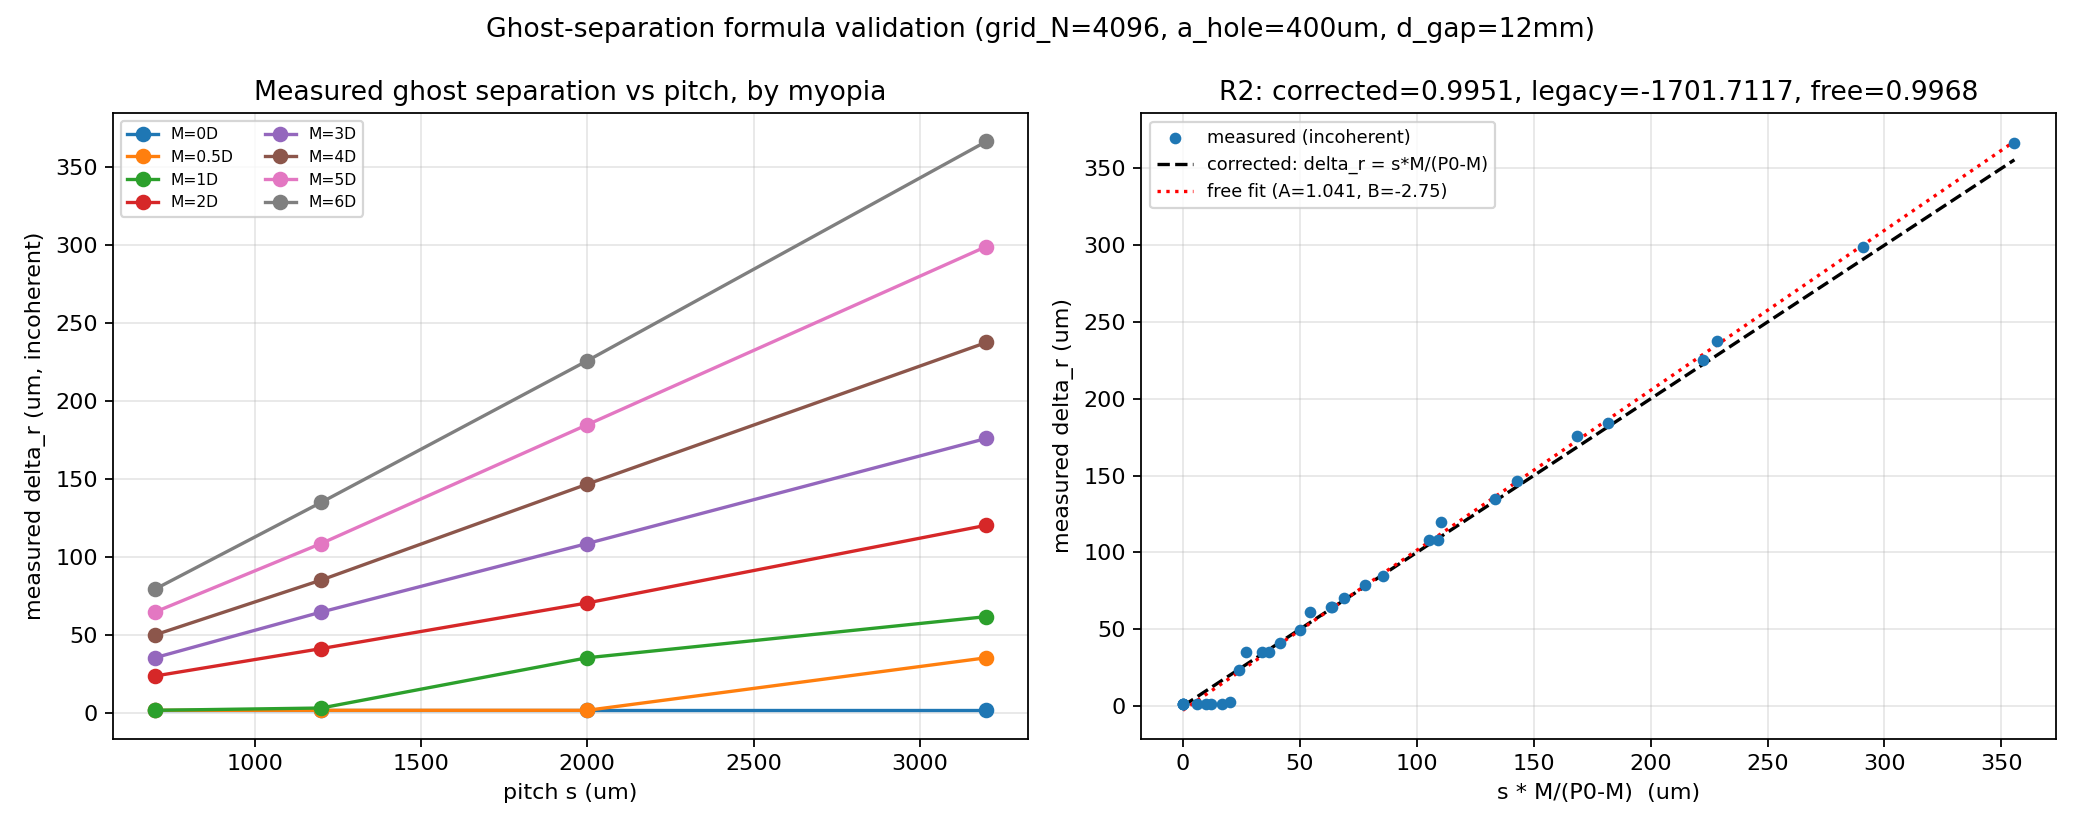
\includegraphics[width=\textwidth]{figures/ghost_formula_validation.png}
\caption{Independent validation of the ghost-separation formula
$\Delta r(s,M)=sM/(P_0-M)$ against measured (incoherent) two-hole separation from a
direct wave-optics simulation ($\mathtt{grid\_N}=4096$, $a_{\mathrm{hole}}=400\,\mu$m,
$d_{\mathrm{gap}}=12$\,mm), sweeping pitch $s$ at 8 myopia powers ($M=0$--$6$D). Right
panel: $R^2=0.9951$ for the corrected formula, versus $R^2=-1701.7$ for the legacy
formula this project explicitly disproved and stopped using (a negative $R^2$ --
worse than predicting the mean). A free 2-parameter affine fit recovers $A=1.041$,
$B=-2.75\,\mu$m, close to the zero-intercept unit-slope line the physics predicts.
Source: \texttt{Array\_Design/array\_optimization/stage0\_ghost\_validation/}
\texttt{ghost\_formula\_validation.png}, mtime 2026-08-14, the original validation run
this pipeline's own \texttt{engine/ghost\_formula.py} was copied from (byte-for-byte
verified against this same dataset, \texttt{VALIDATION.md}).}
\label{fig:ghost-validation}
\end{figure}

\section{The heuristic-CSF-out-of-range bug and the Barten (1999) fix}
\label{sec:barten}
Evaluating Equation~\ref{eq:three-regime} requires a CSF model. This project's own
first-pass CSF implementation (\texttt{Array\_Design/ghosting/contrast.py}) is a
heuristic, peak-matched to reported CSF peaks at 4--8\,cycles/degree (cpd), and was
\textbf{never fit or validated below its own peak frequency}.

\begin{warnbox}{Pass 1: a physically impossible result, traced to its root cause}
A 36-point sweep (apertures $\{300,400,700,1000\}\,\mu$m $\times$ pitches
$\{700,900,1200,1500,2000,2500,3200,4000,4800\}\,\mu$m, $M=4$D,
$d_{\mathrm{gap}}=12$\,mm, $\lambda=550$\,nm, $D_{\mathrm{pupil}}=4000\,\mu$m,
$N_{\mathrm{grid}}=1024$, square packing) found \textbf{zero} Regime~C points -- every
point classified as A (16/36) or B (20/36), i.e.\ every dense, potentially-dangerous
pitch was classified ``safe.'' Traced to root cause: every Regime-B point had a genuine
ghosting fundamental frequency $f_0<0.3$\,cpd (physically correct -- a near-eye,
millimetre-scale pitch genuinely produces a coarse, sub-1-cpd periodic pattern),
evaluated against the heuristic CSF model \emph{far outside its own fitted range}, which
in that regime returned a physically impossible required-contrast threshold of
16{,}337 to 1{,}000{,}000 (i.e.\ more than 100\% contrast) -- trivially satisfying
Regime~B (``safe'') regardless of the design's real MTF value. Source:
\texttt{Array\_Design/ghosting/RESULTS.md}, ``Pass 1'' section, verified read directly.
\end{warnbox}

\textbf{Fix:} a working implementation of the real Barten (1999) contrast sensitivity
model \citep{barten1999,barten2003} (simplified form via the published
\texttt{colour-science} Python package) was located and verified, with a stated valid
range of 0.2--50\,cpd -- overlapping this project's actual ghosting frequencies
(0.10--0.30\,cpd), unlike the heuristic. Sanity-checked first (threshold 0.6\%--3.6\%
across a 2--60\textdegree{} field-size range at that frequency, near-luminance-independent
-- physically sane behaviour, unlike the heuristic's out-of-range artifact).

\begin{center}
\begin{tabular}{lcc}
\toprule
Regime & Pass 1 (heuristic CSF) & Pass 2 (real Barten CSF) \\
\midrule
A (sparse, $N_{\mathrm{eff}}\le1$) & 16 & 16 (unchanged) \\
B (dense, CSF says safe) & 20 & \textbf{0} \\
C (danger zone) & 0 & \textbf{20} \\
\bottomrule
\end{tabular}
\end{center}
\textbf{Every previously-``safe'' dense point was reclassified as danger zone --
including the entire tested real dense-patent pitch range (700--1200\,$\mu$m).} This
reclassification is directionally consistent with Kim et al.\ (2017)'s directly-quoted
clinical finding above: the theory no longer needs an unresolved gap to explain that
finding away (source: \texttt{Array\_Design/ghosting/RESULTS.md}, ``Pass 2'').

\subsection{Pass 3: the harmonic series, not just the fundamental}
\label{sec:harmonic}
Passes 1--2 tested only the fundamental ghosting frequency $f_0=1/\Delta r$. A finite
train of $N$ shifted PSF copies (Equation~\ref{eq:comb}) is a genuinely periodic signal
with harmonic content at every $n f_0$ ($n=1,2,3,\dots$), not a single sinusoid.
Computing the full harmonic margin profile $\mathrm{MTF}(nf_0)/\mathrm{CSF}^{-1}(nf_0)$
for $n=1$ to $40$ at every dense-pitch test point found the worst-case harmonic is
\textbf{never} $n=1$: for the representative case $a_{\mathrm{hole}}=400\,\mu$m,
pitch $=900\,\mu$m, $M=4$D, the fundamental-alone margin is $75.6$ (already $>1$, i.e.\
already ``danger zone'' under Pass~2), but the actual worst harmonic is $n=9$, at
2.09\,cpd, with margin $329.2$ -- \textbf{4.4$\times$ more dangerous than the
fundamental alone predicted}.

\begin{keybox}{Why this generalizes, not just this one case}
MTF decreases smoothly and monotonically with frequency; the Barten CSF's own
sensitivity peak sits in a fixed \emph{absolute} frequency band ($\sim$2--5\,cpd)
regardless of pitch. The product of a monotonically-falling curve and a fixed-position
peak has its own peak at that same fixed absolute frequency -- changing the array pitch
only determines \emph{which harmonic index} $n$ happens to land near that peak, not
whether one does. Confirmed by re-running the full 36-point sweep with harmonic
analysis: the worst-case margin at a given aperture is essentially constant across
every dense pitch tested ($\sim329$ for $a_{\mathrm{hole}}=300$/$400\,\mu$m, $\sim273$
for $700\,\mu$m, $\sim219$ for $1000\,\mu$m), only the specific harmonic index achieving
it changes. Source: \texttt{Array\_Design/ghosting/RESULTS.md}, ``Pass 3.''
\end{keybox}

\section{Vignetting: gaze-dependent aperture activation}
\label{sec:vignetting}
As the wearer's eye rotates by eccentricity angle $\varphi$ from the array's own
optical axis, the pupil's center shifts laterally relative to the (head-fixed) array by
\begin{equation}
\Delta(\varphi) = R_{\mathrm{rot}}\sin\varphi
\label{eq:pupil-shift}
\end{equation}
with $R_{\mathrm{rot}}=13.5$\,mm (physiological range 13--14\,mm), in an azimuth
$\theta$ that can, physically, be any direction the wearer happens to look (source:
\texttt{Array\_Design/array\_geometry\_lab/array\_calculation/engine/vignetting\_overlap.py},
function \texttt{pupil\_shift\_um}, verified read directly). At each shifted pupil
position, the illuminated area contributed by hole $i$ (radius $R_h$) is the exact
circle--circle overlap area between the pupil disc (radius $R_p$) and that hole's disc,
handled in three explicit regimes with no implicit fallthrough:
\begin{equation}
A_{\mathrm{overlap}}(\Delta_i,R_p,R_h) =
\begin{cases}
\pi\min(R_p,R_h)^2 & \Delta_i \le |R_p-R_h| \quad \text{(full containment)} \\[4pt]
0 & \Delta_i \ge R_p+R_h \quad \text{(no overlap)} \\[6pt]
R_p^2\cos^{-1}\!\Big(\dfrac{\Delta_i^2+R_p^2-R_h^2}{2\Delta_i R_p}\Big)
+ R_h^2\cos^{-1}\!\Big(\dfrac{\Delta_i^2+R_h^2-R_p^2}{2\Delta_i R_h}\Big) & \\
\quad{}-\dfrac12\sqrt{(-\Delta_i+R_p+R_h)(\Delta_i+R_p-R_h)(\Delta_i+R_h-R_p)(\Delta_i+R_p+R_h)}
& \text{otherwise (partial overlap)}
\end{cases}
\label{eq:overlap}
\end{equation}
(Handbook 2, Sec.\ 13.2, implemented verbatim in \texttt{vignetting\_overlap.py}'s
\texttt{overlap\_area\_um2}, verified read directly.)

\begin{keybox}{A floating-point boundary defect, found and fixed}
Near the exact boundary $\Delta_i=R_p+R_h$, floating-point round-off on the two
$\cos^{-1}$ terms in the partial-overlap branch can produce a small \emph{negative}
computed area despite the true area being exactly zero there by construction --
observed concretely as $-0.0589\,\mu\mathrm{m}^2$ at $\Delta_i=3000\,\mu$m for a
$2000\,\mu$m hole. The implementation clamps the square-root term's radicand to
$[0,\infty)$ as a first safeguard, and clamps the final combined area to $[0,\infty)$ as
an independent second safeguard closing the same gap -- both present in the verified
current code, not merely proposed.
\end{keybox}

Independent validation: \texttt{vignetting\_overlap.py}'s copy of this formula (a
deliberate copy, not an import, so the array-geometry pipeline has zero runtime
dependency on the originating module's internals) was checked against its own
72-point validation dataset and reproduces it to \textbf{4.657$\times10^{-10}\,\mu$m$^2$
maximum absolute difference} (tolerance $10^{-6}\,\mu$m$^2$), with zero negative-area
outputs produced -- confirming the boundary-clamp fix was copied along with the formula,
not left behind (source: \texttt{VALIDATION.md}, verified present, this project's own
Part~1 validation gate).

\begin{figure}[htbp]
\centering
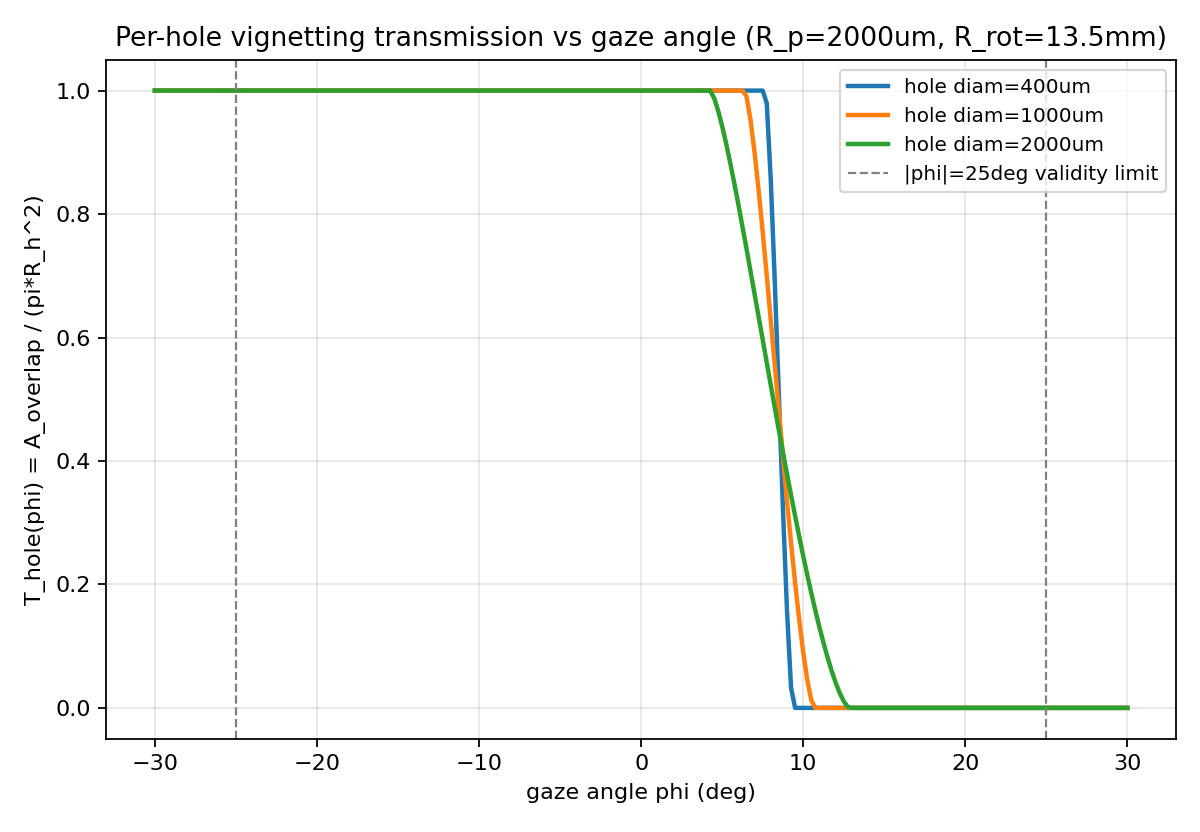
\includegraphics[width=0.75\textwidth]{figures/vignetting_validation.png}
\caption{Per-hole vignetting transmission $T_{\mathrm{hole}}(\varphi)=A_{\mathrm{overlap}}/(\pi
R_h^2)$ vs.\ gaze angle $\varphi$, three hole diameters, $R_p=2000\,\mu$m,
$R_{\mathrm{rot}}=13.5$\,mm. Transmission is exactly $1.0$ (full illumination) until
the pupil begins to slide off the hole, then falls to exactly $0.0$ over a narrow
angular transition -- the sharpness of this cutoff (a few degrees, not a gradual
taper) is what makes vignetting a genuine on/off hazard rather than a smooth
brightness gradient. The dashed vertical lines mark $|\varphi|=25^\circ$, this
formula's (Equation~\ref{eq:pupil-shift}) own stated small-angle validity limit --
Chapter~\ref{ch:model-b}'s $27^\circ$ extrapolated bin sits just outside it, flagged
there as extrapolated, not silently trusted. Source:
\texttt{Array\_Design/array\_optimization/vignetting\_validation.png}, mtime
2026-08-15, the original validation run \texttt{vignetting\_overlap.py} was copied
from.}
\label{fig:vignetting-transmission}
\end{figure}

\subsection{Single-axis vs.\ full-azimuth sampling}
\label{sec:single-axis-limitation}
This project's original vignetting evaluation (\texttt{margins/vignetting\_robustness.py})
models gaze along a \emph{single axis} only -- the pupil shifts to
$(\Delta(\varphi),0)$, never at any other azimuth $\theta$ -- matching the convention of
the module it was derived from. This is a real, acknowledged modelling limitation
(Section~\ref{sec:model-a-limitation}), not an oversight left undocumented: the module's
own docstring states plainly that this convention was inherited, and Model~B
(Chapter~\ref{ch:model-b}) was built specifically to remove it.

\section{Blinding, and the fundamental array trade-off}
\label{sec:blinding}
A gaze direction is \emph{blind} when the total illuminated area across every hole is
exactly zero: $\sum_i A_{\mathrm{overlap}}(\Delta_i(\varphi,\theta),R_p,R_h)=0$ -- no
light reaches the retina at that gaze direction at all, as distinct from a
\emph{ghosting} gaze direction, where two or more holes are simultaneously active
(quantified via the active-hole-fraction threshold of Section~\ref{sec:three-regime}).
These two failure modes trade directly against each other through the array's own
pitch: a denser array (smaller pitch, for a fixed hole size) is less likely to leave any
gaze direction blind, because some hole is more likely to be near the shifted pupil at
any given $(\varphi,\theta)$ -- but a denser array is, by the same token, more likely to
have \emph{two} holes simultaneously within the pupil at once, i.e.\ more likely to
ghost. This project's own real, already-computed data confirms this trade-off is not
merely theoretical: at matched pitch (4000\,$\mu$m, $M=2$D, $a_{\mathrm{hole}}=750\,\mu$m),
a ring-based design with 8 holes per ring achieves lower blind fraction (0.03\%) than
its 6-holes-per-ring counterpart (0.23\%) precisely by pulling ring holes closer
together angularly -- but pays for it with a real 7.58\% time-weighted ghost fraction,
against 0.00\% for the 6-hole variant (Section~\ref{sec:hex-intuition},
Figure~\ref{fig:geom-consequence}). Hexagonal packing is shown in
Chapter~\ref{ch:model-b} to be the one family tested that achieves near-zero on
\emph{both} metrics simultaneously at the same matched spacing, rather than trading one
against the other.

\section{Ghosting theory: full literature review}
\label{sec:ghosting-lit-review}
Section~\ref{sec:ghosting-theory} gave the ghosting derivation in compressed form. This
section expands the literature review behind it in full, reproducing the
citation-fidelity discipline of the source document
(\texttt{Array\_Design/ghosting/THEORY.md}, verified read directly, mtime 2026-08-14
00:36) exactly: every claim below is labelled \textbf{[EXACT]} (a first-principles or
exact identity), \textbf{[PUBLISHED]} (a specific cited result applied as originally
derived), \textbf{[SYNTHESIS]} (a novel combination of citations not itself published as
a unified result), or \textbf{[UNTESTED]} (a claim requiring physical or psychophysical
confirmation this project has not obtained). This labelling convention is preserved
here deliberately, not smoothed into uniform prose, because it is itself part of this
project's own honesty discipline: a reader should be able to tell, claim by claim,
which statements in this section are load-bearing established physics and which are
this project's own proposed synthesis.

\subsection{Motivation: two real, sold products the original criterion could not explain}
An early criterion for this project treated adjacent holes at pitch $s$ as producing
retinal images separated by $\Delta r\approx s\,v_r/d_{\mathrm{gap}}$
\textbf{[EXACT, as originally labelled -- see below]}, and called a design ``ghost-free''
when $\Delta r$ was smaller than the single-hole blur radius $r_{EE}(P)$. Checked
against two real, commercially sold pinhole-eyewear patents -- KR~10-2081511 (pitch
3.2--4.8\,mm) and CN~201716487U (pitch 0.7--1.2\,mm), both with
$d_{\mathrm{gap}}\approx12$\,mm and $v_r\approx22$--$24$\,mm -- this criterion predicted
severe (30$\times$--400$\times$) violations for \emph{both} presumably-functional, sold
products. This direct contradiction between a theoretical prediction and two real
commercial devices is what motivated the full re-derivation this section and
Section~\ref{sec:ghosting-theory} document.

\begin{warnbox}{A label that did not survive re-derivation, kept visible rather than quietly corrected}
Equation~(1) above (the $\Delta r\approx s\,v_r/d_{\mathrm{gap}}$ form) was originally
marked \textbf{[EXACT]} in this project's own working notes. An independent
re-derivation subsequently found this label did not hold -- the formula is used nowhere
in this paper's reported results (Section~\ref{sec:ghosting-theory} uses the corrected
convolution-theorem derivation instead) -- and the source document's own convention is
to leave the original claim, and its original (incorrect) fidelity label, visible in
place with a note pointing to the correction, rather than silently edit history. This
paper follows that same convention here.
\end{warnbox}

\subsection{2.1 Lenslet-array merging theory (Gabor superlens)}
The closest existing precedent for a quantitative multi-channel merging condition in
the optics literature is Gabor-superlens theory (a microlens-array imaging
architecture, originating 1941, with modern quantitative treatments from 2014
\needsverify{exact citation for the specific 2014 treatment referenced in the source
document was not itself recorded there beyond the year -- not independently tracked
down for this paper}): mismatched, non-integer-ratio pitches in a two-array relay cause
imaging channels to, in the cited work's own language, ``unite to form superfocal
lines much smaller in number than the number of microlenses'' \textbf{[PUBLISHED]}.
This is cited here as evidence that the general class of problem -- multiple discrete
optical channels merging or failing to merge into a single perceived image -- is a
solved, quantitatively tractable one in an adjacent field, \emph{not} as a directly
transferable formula: a Gabor superlens is a two-array relay forming a real
intermediate image, physically a different system from a single perforated occluder
imaged directly by the eye's own optics, and no attempt is made in this project to
import the Gabor merging condition as-is.

\subsection{2.2 Direct evidence that multi-aperture ghosting is a real, reported clinical symptom}
The single most important literature finding underlying this section: Kim, Park, Park
\& Chun (2017, \emph{J Korean Med Sci} 32(5):850--857) \citep{kim2017} -- already
present in this project's own vetted citation library
(\texttt{stage4\_human\_vision/literature.py}, and independently used elsewhere in this
paper for a wholly separate purpose, Section~\ref{sec:external-validation}) -- directly
reports, in real human subjects wearing real multi-pinhole glasses, ``discomfort from
after-images such as honeycomb images, horizontal grating, and double or triple
vision'' \textbf{[PUBLISHED, direct quotation from the primary source]}, significantly
worse than for single-pinhole glasses tested in the same study. This finding overturns
the original framing of this project's own investigation: the question this project
initially set out to answer was ``why do real, sold multi-pinhole products show no
reported ghosting problem'' -- and the honest literature answer is that they
\emph{do} report exactly this problem, in a directly-quoted clinical source. The
question this section's derivation (Section~\ref{sec:ghosting-theory}) actually needed
to answer is therefore not ``why is ghosting absent,'' but ``why do the two specific
sold patents checked in Section~\ref{sec:ghosting-theory} not appear to address it
explicitly in their own documentation, and under exactly what geometric conditions does
the symptom become severe.''

\subsection{2.3 An independent real-world statement of the discrete-activation mechanism}
A separate, unrelated US patent (cited in the source document by its own title,
``Method for facilitating pinhole effect...''
\needsverify{full patent number not recorded in the source THEORY.md document beyond
this title fragment -- not independently tracked down for this paper}) states,
entirely independently of anything already in this project's own derivation: ``If two
pinholes are separated by less than the diameter of the pupil aperture, two pencils of
ray\ldots{} form two retinal images. Further, too large of a separation will result in
dead spots\ldots{} while too small\ldots{} will produce multiple images.''
\textbf{[PUBLISHED, direct quotation]}. This is significant specifically because it
states a \emph{discrete precondition} -- whether two or more holes are simultaneously
illuminating the pupil at all -- rather than a continuous margin comparison. This is
exactly the $N_{\mathrm{eff}}$ quantity this project's own active-pairs machinery
(\texttt{margins/active\_pairs.py}, Section~\ref{sec:three-regime}) already computes
via direct discrete-lattice enumeration, independently of this patent. The connection
between the patent's own stated mechanism and this project's own pre-existing
$N_{\mathrm{eff}}$ computation was not recognized until this literature review was
written -- i.e.\ this project's own Regime-A criterion ($N_{\mathrm{eff}}\le1$,
Equation~\ref{eq:three-regime}) turns out to be independently corroborated by real
patent-literature language describing the identical physical mechanism, discovered
after the fact rather than designed to match it.

\subsection{2.4 Periodic-artifact visibility: the screen-door-effect precedent}
Display engineering has a standard, mature treatment of an analogous problem: the
visibility of a display's own pixel/subpixel grid structure (the ``screen-door
effect''), which is assessed by expressing the grid's periodicity in cycles per
degree of visual angle, determining the resulting pattern's modulation depth, and
comparing that modulation depth against the human contrast sensitivity function's own
threshold at that spatial frequency \textbf{[PUBLISHED]}. This confirms that the
three-regime criterion's own frequency-domain framework
(Section~\ref{sec:ghosting-theory}, Equation~\ref{eq:three-regime}) is the same
established methodology display engineering already uses for a structurally analogous
periodic-artifact-visibility problem, not a bespoke construction invented for this
project alone. The same literature also confirms that a cruder, acuity-only rule (of
the same general type as this project's own original, later-superseded criterion,
Section~\ref{sec:ghosting-theory}) is a common, recognized first-pass approximation in
that adjacent field too -- i.e.\ this project's own original mistake was not a mistake
unique to this project, but a documented, recurring simplification in the broader
periodic-visual-artifact literature, corrected here by the same frequency-domain
methodology that field already uses to correct it.

\subsection{Synthesis: the three-regime criterion, and what remains untested}
Combining 2.2's discrete-activation precondition, 2.3's independent confirmation of the
same mechanism, and 2.4's frequency-domain visibility methodology, with this project's
own convolution-theorem derivation (Section~\ref{sec:ghosting-theory}), yields
Equation~\ref{eq:three-regime}'s three-regime criterion \textbf{[SYNTHESIS]} -- a novel
combination of these separately-published pieces, not itself a result published as a
unified criterion anywhere in the cited literature. The predicted danger-zone mechanism
(Regime C) is directionally consistent with Kim et al.'s directly-quoted clinical
symptom report (2.2 above), but this consistency is \emph{directional}, not a
quantitative validation: this project has not obtained psychophysical confirmation that
the specific Barten-CSF threshold crossing computed in
Section~\ref{sec:barten}--\ref{sec:harmonic} predicts \emph{which specific} real
designs a real wearer would report symptoms for, only that the general mechanism and
its general conclusion (dense real patent pitches are more dangerous than a
heuristic CSF model suggested) point the same direction as the one directly-quoted
clinical source available \textbf{[UNTESTED]} -- stated here explicitly as a limitation
of this specific sub-claim, in addition to the broader limitations already catalogued
in Chapter~\ref{ch:limitations}.

\section{Full generator equations for all eleven families}
\label{sec:all-generators}
Section~\ref{sec:array-repr} gave the two most-used families (square, hexagonal) in
full. This section derives all eleven implemented families
(\texttt{array\_calculation/generators/}, verified read directly file-by-file; mtimes
in Chapter~\ref{ch:provenance}), since Chapters~\ref{ch:model-a}--\ref{ch:model-b}
evaluate every one of them and Section~\ref{sec:hex-intuition}'s symmetry argument only
has force once the alternatives are actually written down.

Every generator shares one post-processing step, \texttt{base\_generator.finalize()}
(verified read directly): greedy overlap rejection (points are kept in generation
order, any later point closer than $a_{\mathrm{hole}}$ to an already-kept point is
discarded), then recentering on the surviving set's own centroid. This shared step is
the reason a truncated (non-lattice-complete) candidate set can end up off-centre --
the mechanism behind Section~\ref{sec:centered-bug} below -- and is stated once here
rather than repeated in every family's own derivation.

\subsection{Square}
\begin{equation}
(x_{m,n}) = R(\theta_0)\cdot p\,(m,n), \qquad (m,n)\in\mathbb{Z}^2
\end{equation}
Free parameter: pitch $p$ (nearest-neighbor spacing), plus optional rotation
$\theta_0$. Construction: a square meshgrid large enough to contain $N$ points,
radially sorted by distance from the origin, the closest $N$ kept, then rotated by
$\theta_0$ (rotation is applied \emph{after} the radial sort, so it changes only each
point's $(x,y)$, never which points are selected -- rotation preserves every pairwise
and every origin distance exactly).

\subsection{Hexagonal}
\begin{align}
y_r &= r\,p\,\frac{\sqrt3}{2}, \qquad r\in\mathbb{Z} \\
x_{r,m} &= mp + \begin{cases}p/2 & r\text{ odd}\\0&r\text{ even}\end{cases}, \qquad m\in\mathbb{Z}
\end{align}
Row height $p\sqrt3/2$ and alternate-row half-pitch offset are the standard hexagonal
close-packing construction; identical radial-sort-then-keep-closest-$N$ selection as
square.

\subsection{Rectangular}
\begin{equation}
(x_{m,n}) = R(\theta_0)\cdot(mp_x, np_y), \qquad (m,n)\in\mathbb{Z}^2
\end{equation}
Independent $x$- and $y$-pitches $p_x,p_y$. At $p_x=p_y$ this reduces to \emph{exactly}
the same lattice as square's own construction -- the two generators use deliberately
structurally identical code (same meshgrid-then-radial-sort approach) specifically so
this equivalence holds exactly, not approximately, and is checked directly in
\texttt{spot\_check\_generators.py}.

\subsection{Concentric}
\label{sec:concentric-family}
Ring $k=0$ is a single hole at the origin. Ring $k\ge1$ sits at radius $r_k=k\,s$ (ring
spacing $s$) with
\begin{equation}
n_k = \mathrm{round}(n_0\,k), \qquad
\theta_{k,j} = \frac{2\pi j}{n_k},\ j=0,\dots,n_k-1
\end{equation}
hole count \emph{scaling with ring circumference} (constant angular spacing between
adjacent holes on every ring, equal to ring 1's own spacing $2\pi/n_0$) rather than a
fixed count per ring -- a fixed count would make outer rings implausibly sparse or
force inner-ring holes closer than $a_{\mathrm{hole}}$ (which \texttt{finalize()}'s
overlap rejection would then discard anyway), so the constant-angular-spacing rule is
the more physically sensible default for a fabricatable pattern (source: module
docstring, this exact reasoning, verified read directly).

\subsection{Ring-offset concentric}
\label{sec:ring-offset-family}
Identical ring radius/count formula to Section~\ref{sec:concentric-family}, with one
addition: odd-indexed rings ($k$ odd) receive a fixed half-angular-step rotation
$\pi/n_k$ relative to their unrotated position; even rings receive none --
\begin{equation}
\theta_{k,j} = \frac{2\pi j}{n_k} + \begin{cases}\pi/n_k & k\text{ odd}\\0&k\text{ even}\end{cases}
\end{equation}
the ``brick-course'' pattern: adjacent rings' holes sit staggered rather than radially
aligned. An \emph{alternating} offset (not a progressively-accumulating one) was
chosen as the more literal reading of a brick pattern -- real brick courses alternate,
they do not progressively drift -- and because it is the simpler, unambiguous
construction; a progressive variant was considered and explicitly not implemented,
per the module's own stated reasoning against shipping an unused second flag.

\subsection{Concentric-centered, and a real, documented bug it exists to fix}
\label{sec:centered-bug}
Investigating this family's own motivation directly (rather than assuming it), its
author found that \texttt{concentric.py} and \texttt{ring\_offset\_concentric.py}
\emph{already} start their own point list with a literal centre hole at $(0,0)$ -- so
the reason neither family's \emph{final}, post-\texttt{finalize()} output has a hole at
the origin is not a missing centre point, but \texttt{base\_generator}'s own shared
recentering step: a \emph{complete} ring sums to exactly $(0,0)$ by rotational
symmetry and never disturbs this, but a \emph{truncated} final ring (the common case,
whenever the requested $N$ does not exactly fill an integer number of complete rings)
does not sum to zero, and the shared recenter-on-centroid step then shifts the nominal
centre hole away from the true origin by exactly that leftover imbalance.

\begin{warnbox}{Confirmed against a real, already-fabrication-relevant case}
\texttt{ring\_offset\_concentric}'s own $N=20$, ring spacing $4000\,\mu$m, $n_0=8$
candidate -- its real $M=2$--$3$D winner in an earlier evaluation pass -- has its
nominal centre hole recentred to \textbf{$1704.8\,\mu$m} from the true origin.
Reproduced bit-for-bit by a naive ``prepend then recenter together'' re-implementation,
confirming this mechanism directly, not by inference.
\end{warnbox}

\textbf{Fix, and the one substantive difference this generator adds}: recenter the
ring points on their \emph{own} centroid first, \emph{then} prepend the $(0,0)$ centre
hole, \emph{then} run \texttt{finalize()} once more on the combined set. Since the ring
points are already exactly zero-mean before the centre hole is added, and the centre
hole itself contributes $(0,0)$ to any mean, the combined set's mean is exactly
$(0,0)$ by construction -- the final recentering step becomes provably a no-op. Checked
directly on the identical displaced case above: centre-hole displacement drops to
$1.6\times10^{-13}\,\mu$m (floating-point noise), confirming the fix, not merely
asserting it.

\subsection{Archimedean spiral}
$r=c\theta$ (unwrapped, not reduced mod $2\pi$) -- the curve where each full
revolution increases $r$ by the constant amount $2\pi c$. Points are placed along the
curve at approximately constant arc-length spacing: since $ds/d\theta=\sqrt{r^2+c^2}$
for this curve, a first-order (Euler) angular step
\begin{equation}
d\theta = \frac{a_{\mathrm{hole}}\cdot f_{\mathrm{spacing}}}{\sqrt{r^2+c^2}}
\end{equation}
(evaluated at the current $r$ before each step, $f_{\mathrm{spacing}}=1.5$ by default)
keeps successive points near-evenly spaced along the arc. Explicitly \emph{not} the
same construction as the Fibonacci/golden-angle family below -- this generator advances
along one continuous outward-spiralling arm; the golden-angle family jumps by a fixed
large irrational angle each step and never traces a continuous curve at all. Confirmed
different point clouds directly, not merely by differing formulas
(\texttt{spot\_check\_generators.py}'s archimedean-vs-fibonacci difference check).

\subsection{Fibonacci (Vogel) spiral and golden-angle phyllotaxis}
\begin{equation}
r_n = c\sqrt n, \qquad \theta_n = n\,\alpha_g, \qquad \alpha_g = \pi(3-\sqrt5)\approx137.50776^\circ,
\qquad n=1,\dots,N
\end{equation}
$\alpha_g=2\pi(1-1/\varphi)$, $\varphi$ the golden ratio -- the irrational angle that
maximizes packing uniformity for this family (Vogel, 1979). ``Golden-angle
phyllotaxis'' and the ``Fibonacci/Vogel spiral'' are, mathematically, the
\emph{identical} formula -- there is no separate standard point-packing construction in
the literature distinct from this one (the visually different ``nested-squares
Fibonacci spiral'' is an unrelated aesthetic curve, not a packing formula, and is not
what either generator name refers to here). Rather than risk two copies silently
drifting apart under future edits, \texttt{golden\_angle.py} re-exports
\texttt{fibonacci\_spiral.generate()} directly under its own family label; for the same
$(N,a_{\mathrm{hole}},c)$ the two generators' output coordinates are, by construction,
identical.

\subsection{Poisson-disk (blue-noise)}
Stochastic; minimum pairwise distance $r=a_{\mathrm{hole}}f_{\mathrm{spacing}}$
enforced via Bridson's algorithm (Bridson, SIGGRAPH 2007 sketches) rather than naive
dart-throwing-with-rejection, whose rejection rate is unbounded as the domain fills
(each new random dart becomes increasingly likely to land too close to an existing
point). Bridson's method instead grows the set from an active frontier -- only ever
proposing new candidates in the annulus $[r,2r]$ around an existing active point,
checked against neighbours via a background grid of cell size $r/\sqrt2$ (small enough
that each cell holds at most one sample) -- and terminates deterministically once no
active point can produce a valid candidate after $k=30$ tries, giving $O(1)$ amortized
work per accepted or retired point rather than the unbounded degradation of naive
rejection sampling. The domain is filled to near-maximal packing, then the $N$ points
closest to the origin are kept (same selection convention as square/hexagonal). Because
the algorithm is stochastic, \texttt{seed} is a required, not optional, parameter for
every call to be reproducible.

\subsection{Jittered lattice}
Starts from \texttt{hexagonal.generate()}'s own lattice, then perturbs every hole by a
random offset sampled \emph{uniformly by area} within a disk of radius
$f_{\mathrm{jitter}}\,p$:
\begin{equation}
\rho = f_{\mathrm{jitter}}\,p\,\sqrt{u}, \qquad u\sim\mathrm{Uniform}(0,1), \qquad
\phi\sim\mathrm{Uniform}(0,2\pi)
\end{equation}
The $\sqrt{u}$ is load-bearing, not optional: sampling the offset magnitude directly as
$f_{\mathrm{jitter}}\,p\,u$ would over-concentrate perturbed points near zero offset,
since area scales as $r^2$, not $r$ -- the same disk-sampling construction already used
elsewhere in this project's own Monte Carlo validation work
(\texttt{array\_optimization/vignetting.py}). A \emph{uniform}, not Gaussian, offset
distribution was chosen specifically because the parameter's own contract is ``offset
up to $f_{\mathrm{jitter}}\,p$'' -- a hard, stated bound; a Gaussian has unbounded
support, which would make that ``up to'' contract false in the tail, however unlikely.
The jittered set is then re-run through \texttt{finalize()}'s own overlap rejection
(jitter can push two holes that were exactly at the lattice's own valid spacing closer
than $a_{\mathrm{hole}}$ -- these must be rejected exactly as any other overlapping
candidate would be, not silently kept because they originated from a valid lattice).
At $f_{\mathrm{jitter}}=0$ every offset is identically zero, so this reduces exactly to
\texttt{hexagonal.generate()}'s own output -- checked directly, not merely argued, in
\texttt{spot\_check\_generators.py}.

\chapter{Evaluation Model A: The Single-Axis Worst-Case Gate}
\label{ch:model-a}

Model A is this project's original array-safety evaluation: for each candidate design,
apply three independent pass/fail gates, then rank surviving candidates by packing
density. It was this project's primary standard until an explicit methodology change on
2026-09-13 (Chapter~\ref{ch:model-b}) promoted Model~B in its place; Model~A's own
results remain valid and are still fully reported here, not deleted, per this project's
own stated policy of keeping superseded models available for comparison.

\section{The three gates}
\label{sec:three-gates}
Implemented in \texttt{array\_evaluation/comparison\_metric/gates.py} (verified read
directly, current file):

\begin{align}
\text{Ghost safety:}\quad & \text{worst\_case\_ghost\_margin} \ge
\frac{2.0\times2.9297\,\mu\mathrm{m}}{\text{resolvable\_blur\_um}} \\
\text{Vignetting safety:}\quad & \text{worst\_case\_vignetting\_margin} \ge
\frac{2.0\times2.9297\,\mu\mathrm{m}}{\text{resolvable\_blur\_um}} \\
\text{Viability:}\quad & \text{min\_illuminated\_area\_across\_}\varphi \ge
0.20\times\pi\Big(\frac{a_{\mathrm{hole}}}{2}\Big)^2
\end{align}
The margin threshold's numerator, $2.9297\,\mu$m, is $2\times$ the ghost-formula
validation grid's own pixel pitch ($1.46\,\mu$m -- the same measurement floor noted in
Section~\ref{sec:vignetting}), i.e.\ twice the finest resolution at which the underlying
ghost-separation formula was itself validated; the $2.0\times$ safety multiple on top of
that is applied per this project's own stated design brief, not independently derived.
The viability floor (20\% of one hole's own full area) requires that floor to hold at
\emph{every} tested gaze angle $\varphi$, not merely at $\varphi=0$ -- an audit fix
documented in \texttt{gates.py}'s own module docstring as replacing an earlier, weaker
``margin $>0$'' check with this real, sourced threshold.

\section{The single-axis limitation, acknowledged}
\label{sec:model-a-limitation}
Model A's ghost and vignetting margins are computed via
\texttt{margins/vignetting\_robustness.py}, which samples gaze along a \emph{single
axis} only ($\theta=0$ always -- Section~\ref{sec:single-axis-limitation}). This is a
genuine limitation, not merely a simplification: for a ring-based family in particular,
a complete blackout can occur in the angular \emph{gap} between two ring holes at one
azimuth while an adjacent azimuth at the identical eccentricity sits directly on top of
a hole -- single-axis sampling can silently miss this. A concrete, real instance of
exactly this failure mode was found in this project's own development: a
\texttt{concentric\_centered} candidate that outperformed the then-current winner
everywhere inside $15^\circ$ failed Model A's worst-case safety gate specifically via a
complete blackout in the $20$--$25^\circ$ gaze range (source:
\texttt{Array\_Design/array\_geometry\_lab/array\_data/evaluation\_results/CENTERED\_CONCENTRIC\_COMPARISON.md},
2026-08-17, verified present) -- the concrete, real-world motivating example for
building Model B's full-azimuth sampling (Chapter~\ref{ch:model-b}).

\section{Current results}
\label{sec:model-a-results}
Winner per myopia power, ranked by packing density among gate survivors (source:
\texttt{Array\_Design/array\_geometry\_lab/array\_data/evaluation\_results/FINAL\_WINNER\_PER\_M.csv},
mtime 2026-09-13 00:42 -- see Chapter~\ref{ch:provenance} for the full provenance
record):
\begin{center}
\begin{tabular}{ccccc}
\toprule
$M$ (D) & Family & $a_{\mathrm{hole}}$ ($\mu$m) & $N$ & Worst-case margins \\
\midrule
0 & square & 2000 & 9 & $\infty/\infty$ \\
1 & square & 1250 & 100 & $\infty/\infty$ \\
2 & square & 750 & 100 & $\infty/\infty$ \\
3 & square & 750 & 100 & $\infty/\infty$ \\
4 & square & 600 & 50 & $\infty/\infty$ \\
5 & square & 600 & 50 & $\infty/\infty$ \\
6 & square & 500 & 50 & $\infty/\infty$ \\
8 & square & 400 & 50 & $\infty/\infty$ \\
\bottomrule
\end{tabular}
\end{center}
An infinite margin means zero simultaneously-illuminated hole pairs at every
single-axis-tested gaze angle -- a structural, geometric guarantee under the single-axis
sampling convention, not a narrowly-cleared numeric threshold. This structural safety is
exactly why Model A alone did not surface the real ring-family blackout of
Section~\ref{sec:model-a-limitation}: a design can be structurally safe along the one
tested axis while still failing badly off it.

\begin{figure}[htbp]
\centering
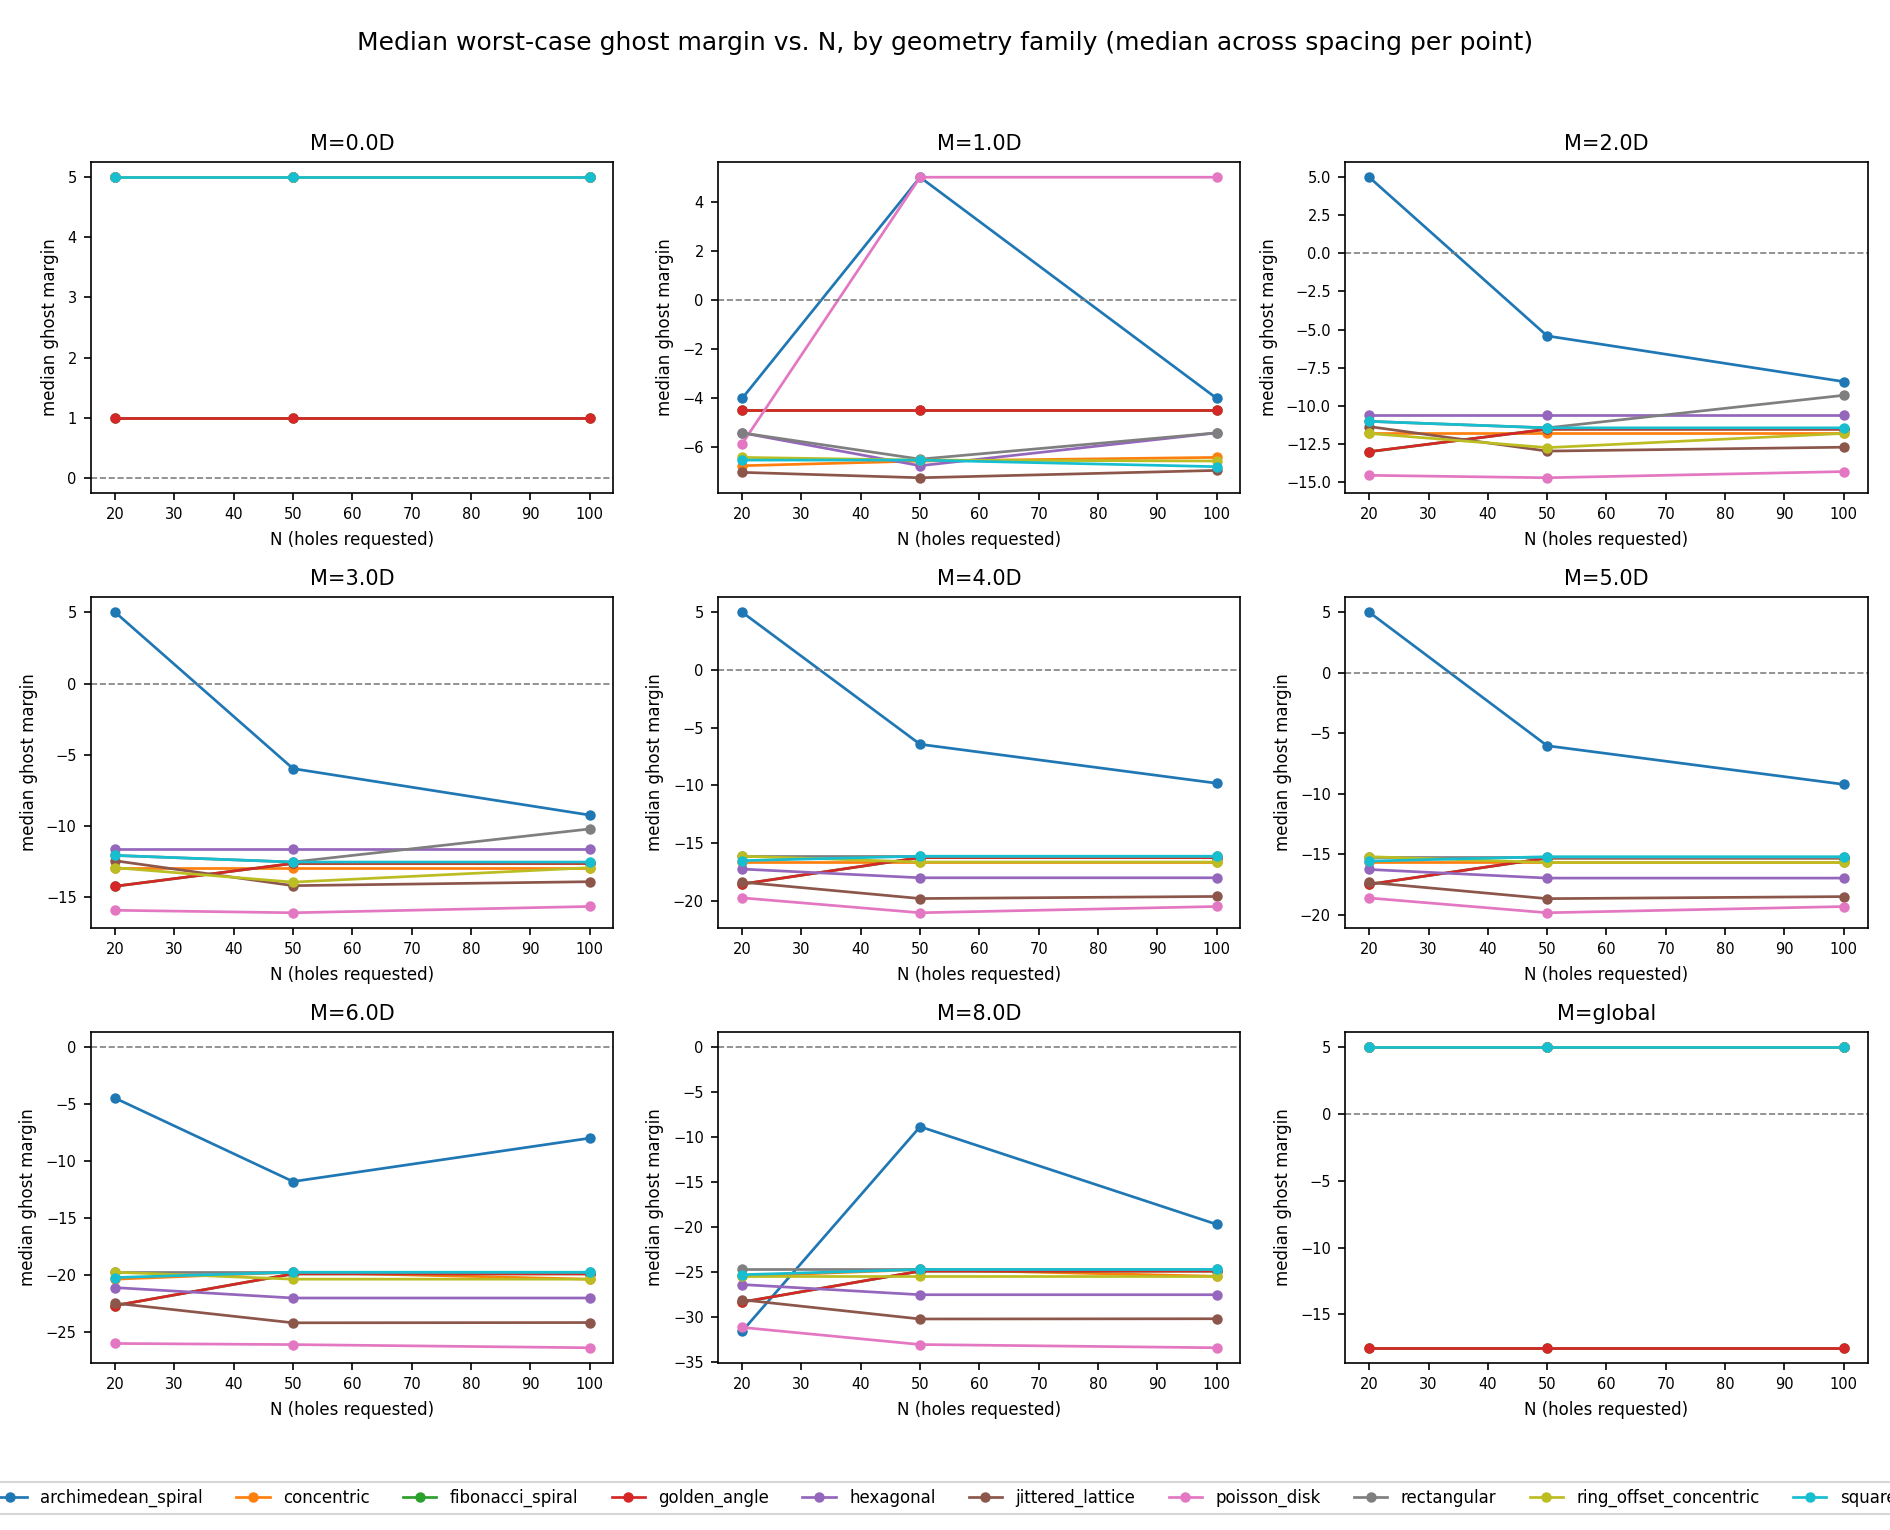
\includegraphics[width=\textwidth]{figures/family_ranking_margin_vs_N.png}
\caption{Median worst-case ghost margin vs.\ $N$ (holes requested), all 11 geometry
families, every $M$ and the global scope -- the full picture behind the winner table
above. Square (cyan) and, separately, golden\_angle (red) are the only families that
stay non-negative at $M=0$D and global scope; at every other $M$, square is again the
only family that survives with a positive/infinite margin, while most of the
remaining 9 families sit well below the $y=0$ safety line regardless of $N$ --
visual confirmation that Model A's structural-safety requirement is a genuinely
narrow target, not an easy bar most designs clear. Source:
\texttt{array\_data/evaluation\_results/family\_ranking\_margin\_vs\_N.png}, mtime
2026-09-13 00:37 (pre-generated by this project's own \texttt{family\_ranking}
analysis, not produced for this paper).}
\label{fig:family-ranking-margin}
\end{figure}

\chapter{Evaluation Model B: Two-Dimensional Gaze-Weighted Evaluation}
\label{ch:model-b}

\section{Methodology change}
On 2026-09-13, following an explicit project decision, gaze-weighted (time-weighted
ghost/blind fraction) evaluation was promoted from a secondary, comparison-only
analysis to this project's \textbf{primary} array-safety standard, judged more
realistic than a pure worst-case-across-every-tested-gaze-angle criterion (source:
\texttt{Array\_Design/array\_geometry\_lab/GAZE\_WEIGHTED\_APPROACH.md}, ``UPDATE,
2026-09-13'' section, and
\texttt{array\_data/evaluation\_results/TIMELINE.txt}, both verified present, mtime
2026-09-13 14:10--14:11). Model~A (Chapter~\ref{ch:model-a}) was not deleted or edited
-- it remains valid, fully reported data -- but is no longer this project's headline
answer.

\section{Full-azimuth, gaze-time-weighted sampling}
\label{sec:model-b-method}
Model B removes Model A's single-axis limitation (Section~\ref{sec:model-a-limitation})
directly: for each of 26 eccentricity bins (bin centers $0.5^\circ$ to $27.0^\circ$,
weighted by an empirically measured eccentricity distribution -- \%
of viewing time per bin, summing to $100.0\%$, cumulative $51.61\%$ by $6^\circ$ and
$95.27\%$ by $17^\circ$, checked to satisfy both cumulative checkpoints before any sweep
runs), the pupil is sampled at $N_\theta=36$ azimuths uniformly around the full circle,
using the same validated radial-shift magnitude (Equation~\ref{eq:pupil-shift}) applied
in an arbitrary direction: $\mathrm{pupil\_center}=(R\cos\theta,R\sin\theta)$.

\begin{keybox}{The $27^\circ$ bin is explicitly flagged as extrapolated}
The eccentricity distribution's own highest bin is centered at $27^\circ$ (0.58\% of
viewing time), \textbf{outside} \texttt{vignetting\_overlap.py}'s own stated small-angle
validity range for the pupil-shift formula, $|\varphi|\le25^\circ$. The formula does not
numerically diverge there -- it is still evaluated, per the source module's own
docstring, ``the formula doesn't blow up... every caller that reports a number must
check and flag this, not silently trust it'' -- and this paper does exactly that: every
number in this chapter that includes the $27^\circ$ bin is extrapolated beyond the
formula's own validated range, at only 0.58\% total weight, and is flagged here rather
than silently trusted.
\end{keybox}

At each active hole, the illuminated area is the exact overlap area of
Equation~\ref{eq:overlap}; a hole counts as \emph{active} when its own illuminated
fraction exceeds $0.5$ (\texttt{margins/active\_pairs.py}'s
\texttt{DEFAULT\_ACTIVE\_FRAC\_THRESHOLD}, reused unmodified here, so ``ghosting'' means
the identical thing in Model~B as in Model~A). \textit{Blind} is total illuminated area
exactly zero, time-weighted across every sampled $(\varphi,\theta)$ pair, giving
\texttt{time\_weighted\_blind\_pct} and \texttt{time\_weighted\_ghost\_pct} per candidate
(source: \texttt{array\_calculation/compute\_gaze\_weighted\_metrics.py}, verified read
directly).

\section{Adding a hard blindness gate}
\label{sec:blindness-gate}
The primary ranking rule (\texttt{comparison\_metric/primary\_ranking\_gaze\_weighted.py})
hard-gates any candidate with \texttt{time\_weighted\_blind\_pct} above a tolerance,
then minimizes \texttt{time\_weighted\_ghost\_pct} among survivors.

\begin{warnbox}{A strict 0\% blindness gate was tried first and rejected -- checked, not assumed}
A strict $0\%$-blind gate produces a sharp cliff at $M=6$D/$8$D: it forces ghost
percentages up to 27--30\%, because every genuinely-zero-blind candidate at those $M$
carries real ghost, while the best hexagonal candidates there carry only a small
0.12--0.33\% blind time. This is the same ``margin-vs-zero'' failure mode Model~A's own
audit fix (Section~\ref{sec:three-gates}) had already diagnosed once before, in a
different context. A $1.0\%$ tolerance was used instead, which clears every existing
winner's own blind percentage with headroom and produces the identical family choices
as the earlier ungated ranking (hexagonal $M=1$--$6$, square $M=0/8$/global) -- the gate
exists to prevent a \emph{future} re-run from silently accepting a degenerate design, it
did not have to override anything in the current result set.
\end{warnbox}

\begin{figure}[htbp]
\centering
\begin{minipage}{0.32\textwidth}\centering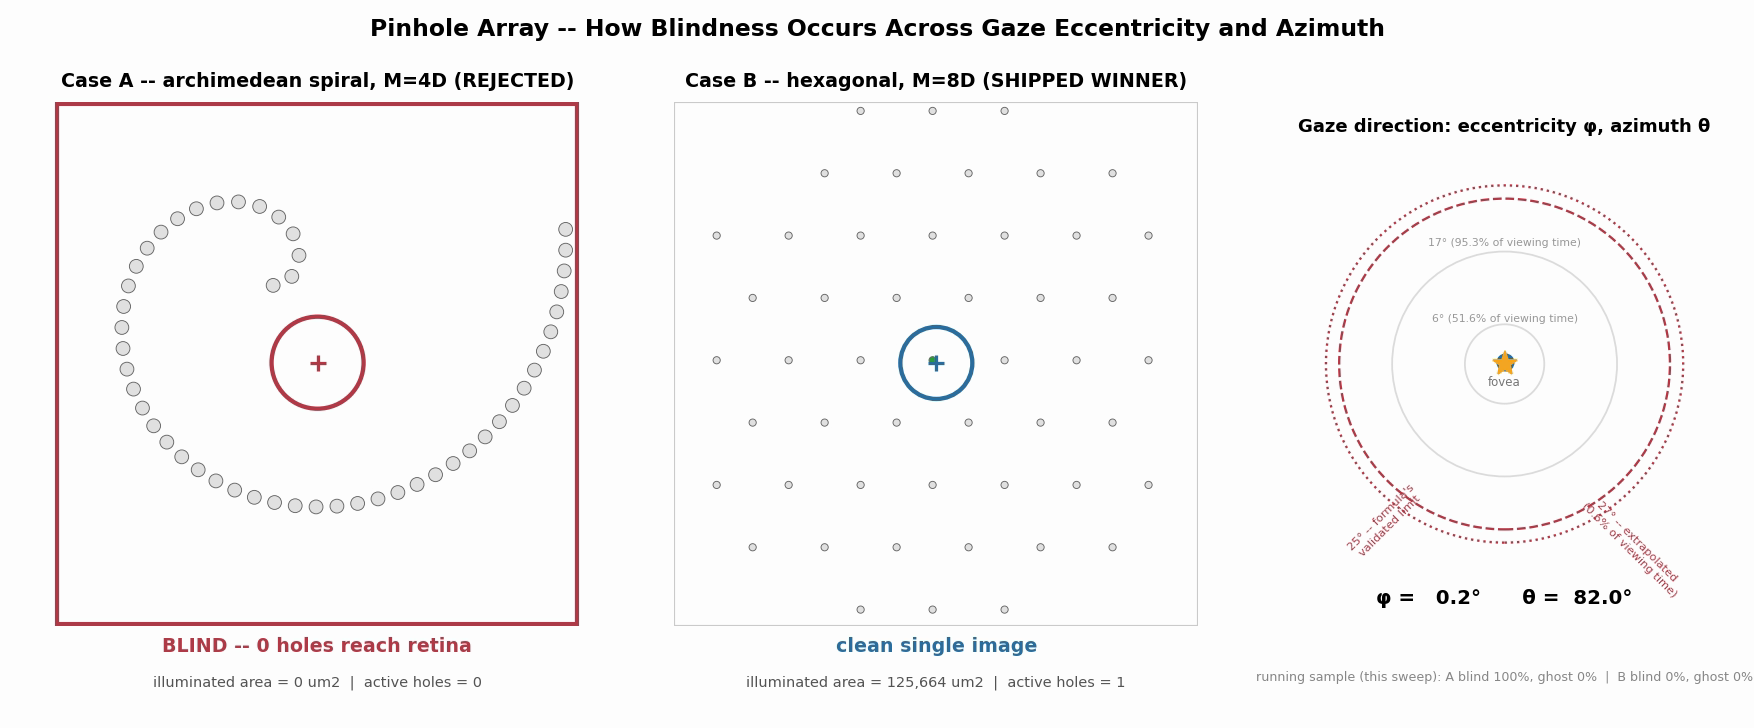
\includegraphics[width=\textwidth]{figures/blindness_frame_blind.png}\end{minipage}\hfill
\begin{minipage}{0.32\textwidth}\centering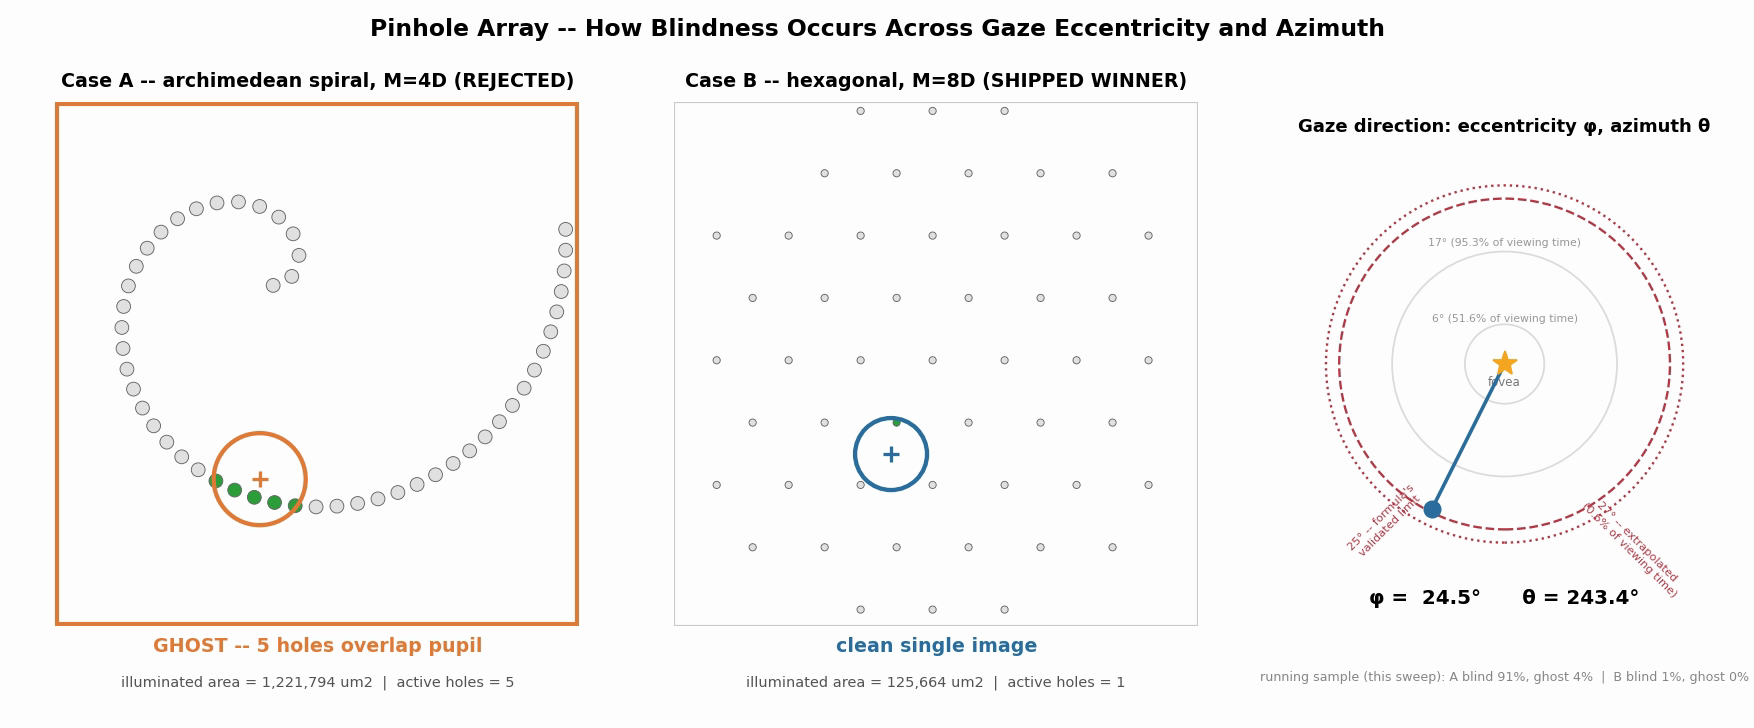
\includegraphics[width=\textwidth]{figures/blindness_frame_ghost.png}\end{minipage}\hfill
\begin{minipage}{0.32\textwidth}\centering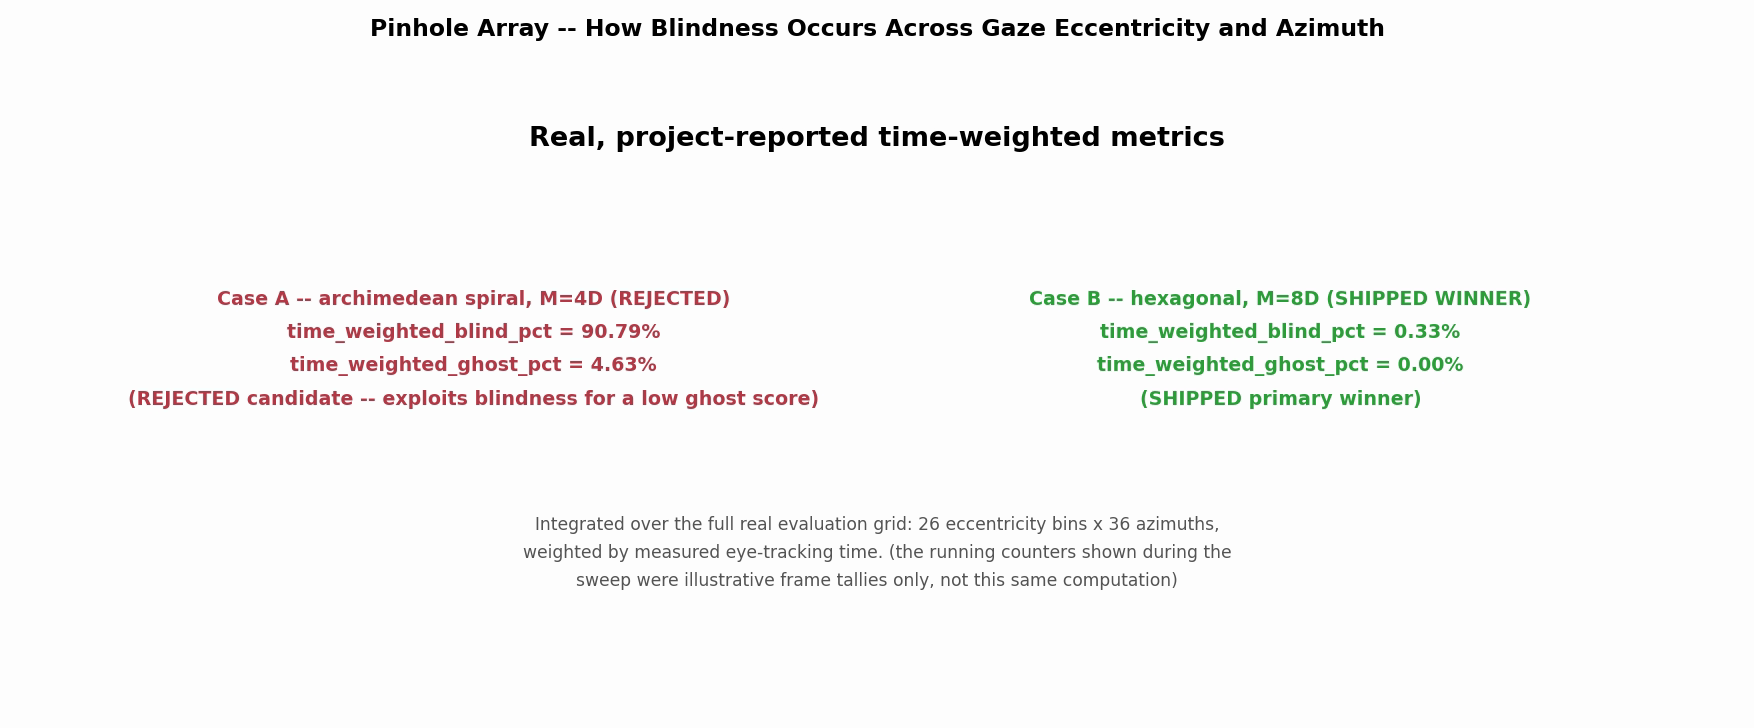
\includegraphics[width=\textwidth]{figures/blindness_frame_clean.png}\end{minipage}
\caption{All three states this section's gate distinguishes, shown side by side for
the same two real candidates swept through the identical $(\varphi,\theta)$ gaze path
-- Case A: \texttt{archimedean\_spiral}, $M=4$D (a real, rejected candidate,
$90.79\%$ time-weighted blind); Case B: the shipped hexagonal $M=8$D primary winner
($0.33\%$ blind). Left: Case~A \textbf{BLIND} ($\varphi=0.2^\circ,\theta=82.0^\circ$,
0 holes reach the retina). Middle: Case~A \textbf{GHOST} (5 simultaneously active
holes at $\varphi=24.5^\circ,\theta=243.4^\circ$) -- note the images coincide near
$\varphi=0$ but a real ghost-separation only appears at higher $\varphi$, consistent
with $\Delta r(s,M)=sM/(P_0-M)$ vanishing only at $M=0$, not at $\varphi=0$. Right:
both cases \textbf{clean}. Frames extracted via \texttt{ffmpeg} from
\texttt{Array\_Design/array\_geometry\_lab/blindness\_mechanism\_animation/}
\texttt{blindness\_mechanism\_animation.mp4} (mtime 2026-09-16 12:58); the underlying
simulation reuses \texttt{engine/vignetting\_overlap.py}'s validated overlap-area
formula and \texttt{engine/ghost\_formula.py}'s validated separation formula
unmodified -- the same two functions used throughout Chapter~\ref{ch:array-theory}.}
\label{fig:blindness-states}
\end{figure}

\section{Current results}
\label{sec:model-b-results}
Source: \texttt{Array\_Design/array\_geometry\_lab/array\_data/evaluation\_results/PRIMARY\_WINNER\_PER\_M.csv},
mtime 2026-09-13 14:10 (the most recent evaluation-results file in its directory as of
this writing; see Chapter~\ref{ch:provenance}).
\begin{center}
\begin{tabular}{cccccc}
\toprule
$M$ (D) & Family & $a_{\mathrm{hole}}$ ($\mu$m) & $N$ & Blind \% & Ghost \% \\
\midrule
0 & square & 2000 & 20 & 0.00 & 0.00 \\
1 & hexagonal & 1250 & 20 & 0.00 & 0.00 \\
2 & hexagonal & 750 & 20 & 0.00 & 0.00 \\
3 & hexagonal & 750 & 20 & 0.00 & 0.00 \\
4 & hexagonal & 600 & 20 & 0.00 & 0.00 \\
5 & hexagonal & 600 & 20 & 0.00 & 0.00 \\
6 & hexagonal & 500 & 100 & 0.12 & 0.00 \\
8 & hexagonal & 400 & 50 & 0.33 & 0.00 \\
\bottomrule
\end{tabular}
\end{center}
Hexagonal packing wins six of eight tested myopia powers; square wins at $M=0$ and the
global (worst-case-across-$M$) scope. Every winning design achieves genuine $0.00\%$
ghost under realistic, time-weighted gaze -- not merely a structural worst-case
guarantee -- and the only two nonzero blind percentages in the table (0.12\%, 0.33\%)
are both well inside the $1.0\%$ gate of Section~\ref{sec:blindness-gate}.

\section{Why hexagonal: the physical intuition}
\label{sec:hex-intuition}
As the eye rotates by $\varphi$, the pupil shifts in \emph{some} azimuth $\theta$ that
could, physically, be any direction the wearer happens to look. A safe array needs small
gaps between holes in every direction, not only a single favoured axis. Three properties
of a hexagonal lattice matter here, all standard results:

\begin{enumerate}
\item \textbf{Densest possible 2D point packing.} Hexagonal packing achieves packing
density $\pi/(2\sqrt3)\approx0.9069$, provably optimal (the honeycomb conjecture) -- for
a given minimum safe pitch, it fits the most holes into that pitch.
\item \textbf{Maximum rotational symmetry for a periodic lattice.} A hexagonal lattice
has 6-fold rotational symmetry -- the \emph{maximum} any periodic 2D lattice can have at
all, by the crystallographic restriction theorem (only 2-, 3-, 4-, and 6-fold rotations
are compatible with translational periodicity). This makes the gap structure between
holes nearly isotropic: it matters comparatively little which azimuth the pupil happens
to shift toward.
\item \textbf{Regular-hexagon Voronoi cells.} The Voronoi cell of a hexagonal lattice
point is a regular hexagon -- the polygon that best approximates a circle while still
tiling the plane with no gaps -- directly minimizing the worst-case distance from any
pupil position to its nearest hole, uniformly in every direction.
\end{enumerate}

A square lattice, by contrast, has only 4-fold symmetry: its diagonal ($45^\circ$)
nearest-neighbor distance is $\sqrt2\times$ its axis-aligned nearest-neighbor distance --
a real, quantifiable weak direction. This is exactly the mechanism behind the concrete
ring-family blackout of Section~\ref{sec:model-a-limitation}: a ring-based design's holes
exist only at discrete angular positions (a fixed \texttt{holes\_per\_ring0} count), with
real angular gaps between them that a single-axis test can miss entirely.

\begin{figure}[htbp]
\centering
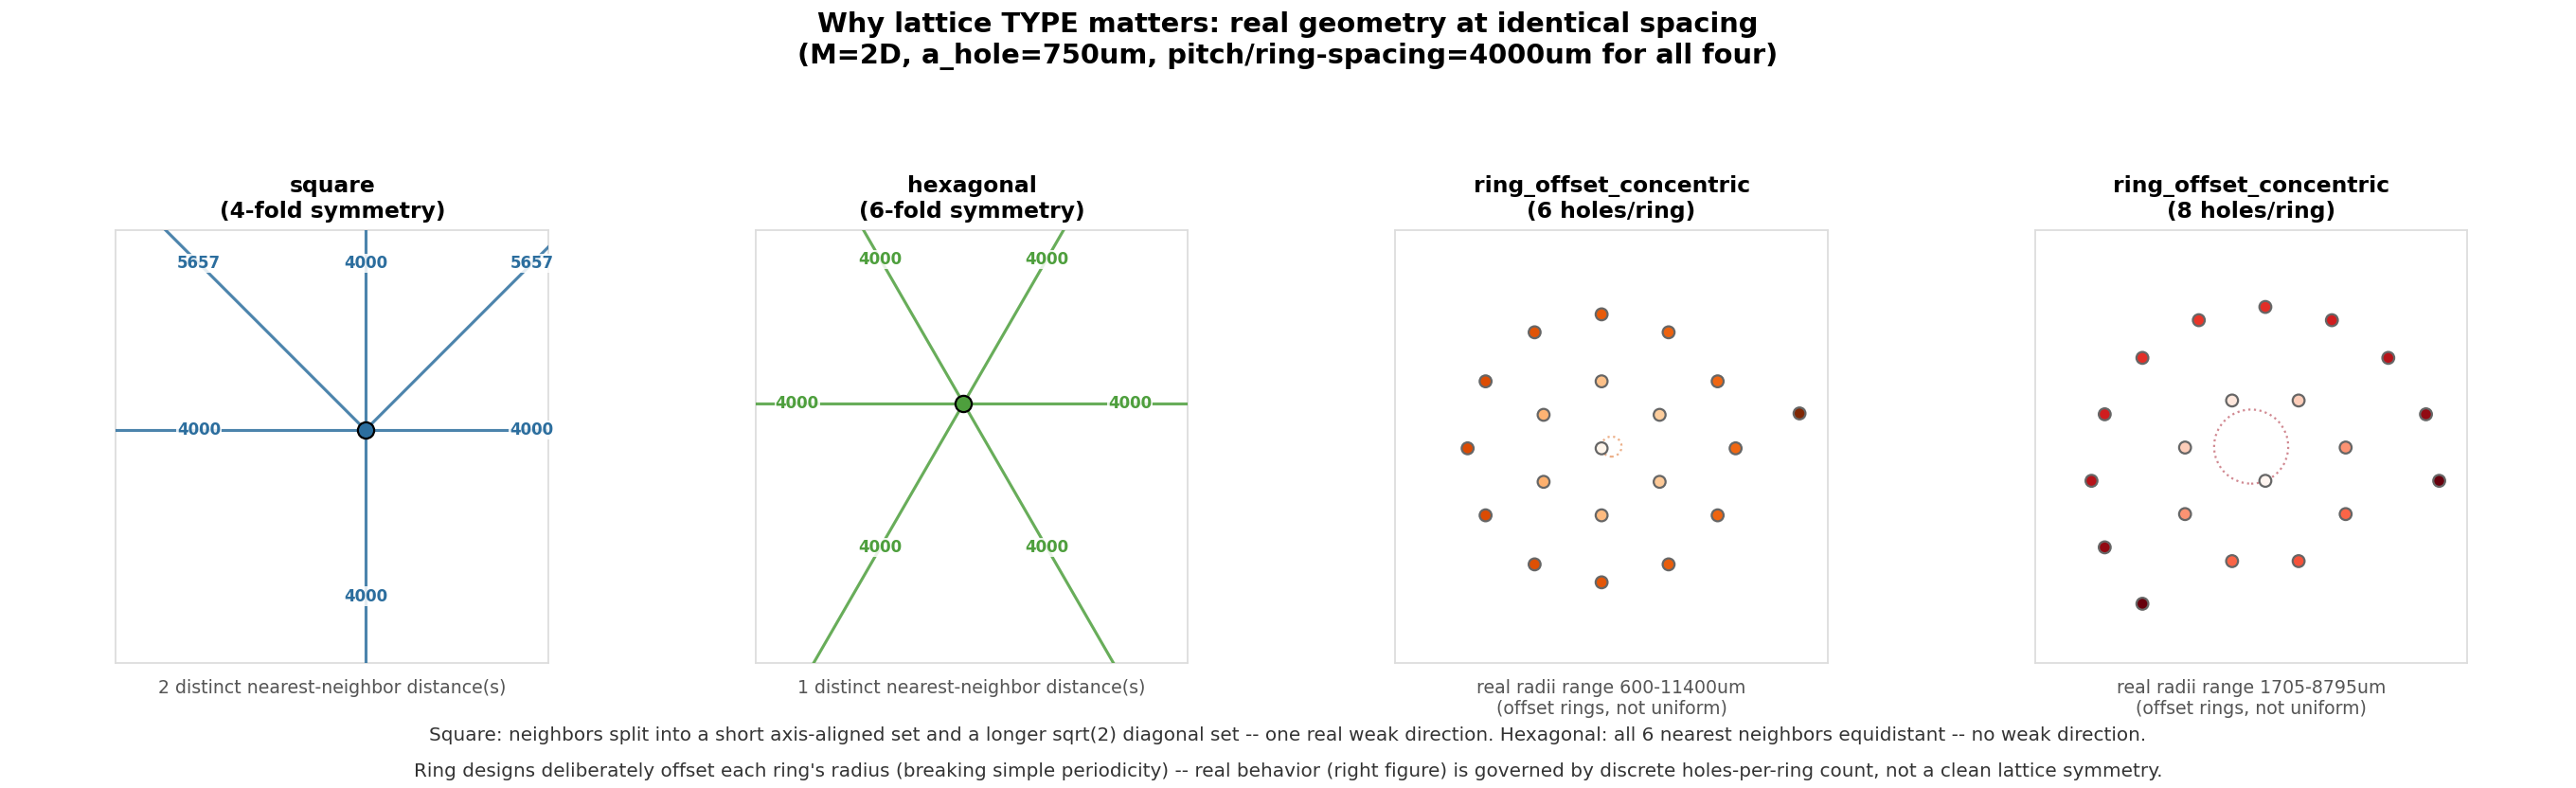
\includegraphics[width=0.95\textwidth]{figures/geometry_intuition_structure.png}
\caption{Real regenerated nearest-neighbor structure at identical spacing
(pitch/ring-spacing $=4000\,\mu$m, $a_{\mathrm{hole}}=750\,\mu$m, $M=2$D). Square: two
distinct nearest-neighbor distances, 4000 and $5657\,\mu$m ($=4000\sqrt2$, confirming the
diagonal weak direction exactly). Hexagonal: one distinct distance, all six neighbors
equidistant. Ring designs (6 and 8 holes/ring): genuinely offset, non-uniform ring
radii, not a simple lattice -- shown as real coordinate scatter rather than forced into
the same distance-count framing. Source: this analysis, regenerated directly from
\texttt{array\_calculation/degeneracy\_filter.py}'s own generator functions; see
Chapter~\ref{ch:provenance}.}
\label{fig:geom-structure}
\end{figure}

\begin{figure}[htbp]
\centering
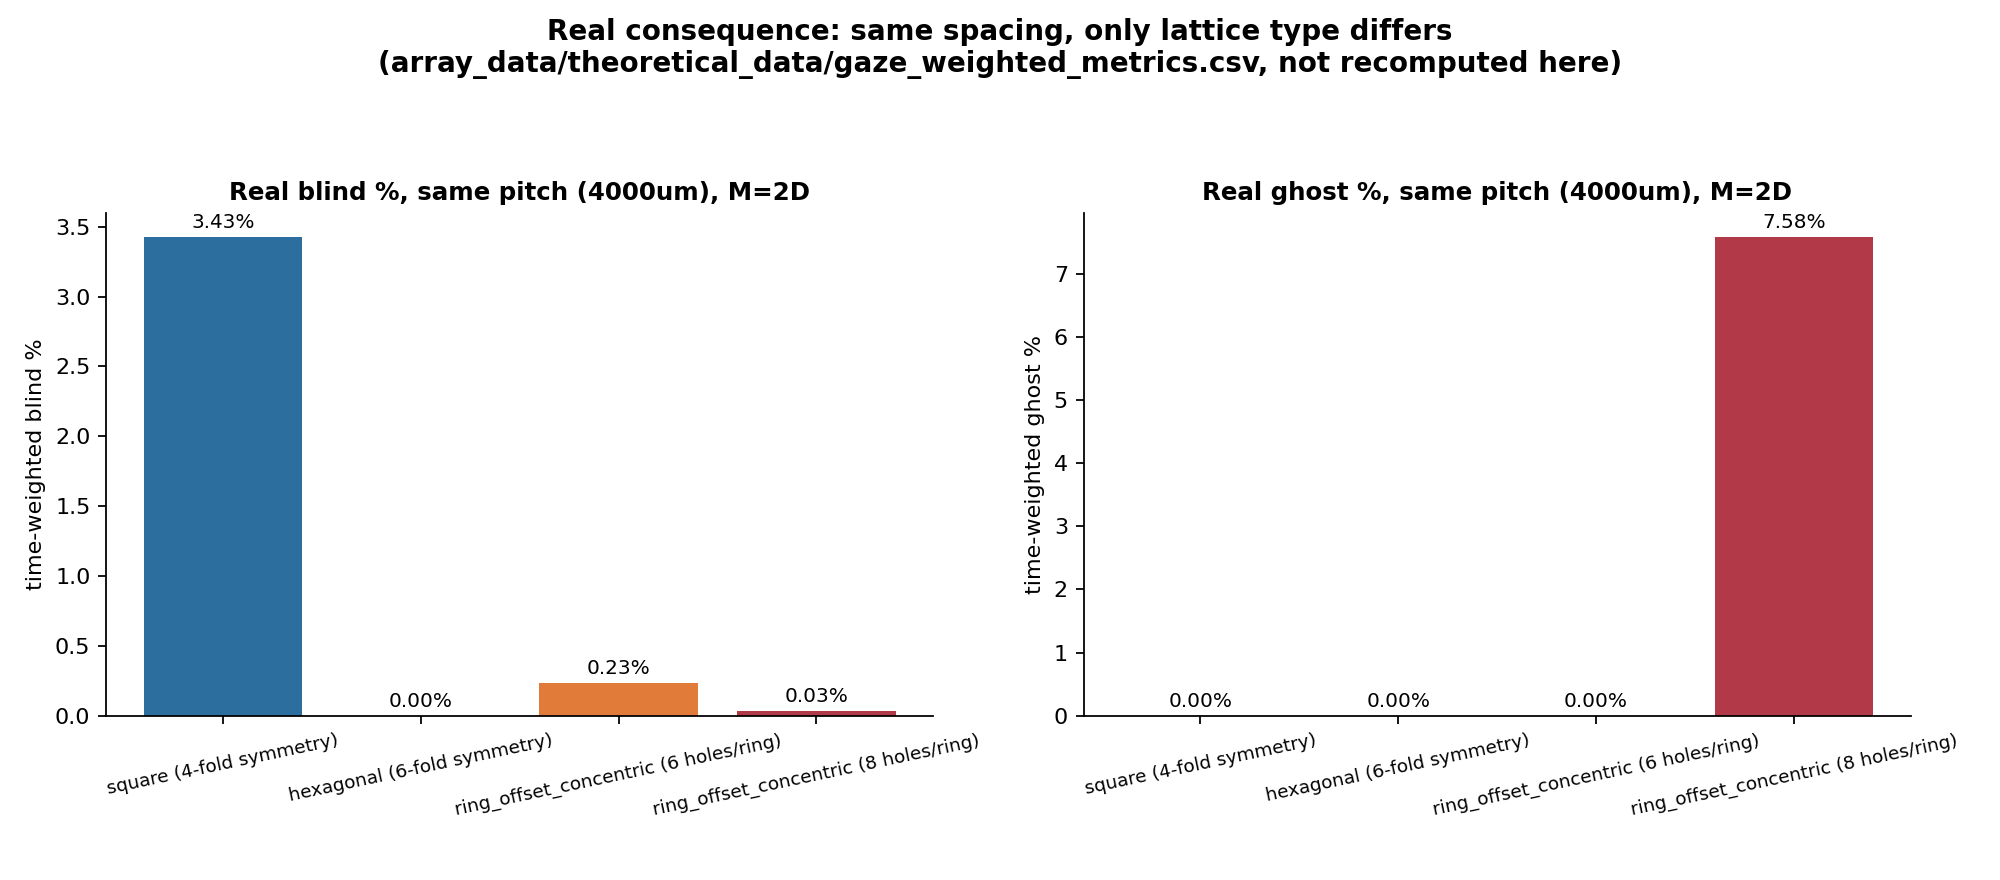
\includegraphics[width=0.85\textwidth]{figures/geometry_intuition_real_consequence.png}
\caption{Real, already-computed gaze-weighted blind\%/ghost\% for the same four
matched-spacing designs as Figure~\ref{fig:geom-structure}, read directly from
\texttt{array\_data/theoretical\_data/gaze\_weighted\_metrics.csv} (not recomputed for
this figure). Hexagonal is the only design with $0.00\%$ on both axes simultaneously;
the ring-of-8 design trades blind\% for a real $7.58\%$ ghost fraction -- the discrete
angular-gap tension (Section~\ref{sec:blinding}) hexagonal packing avoids by being
simultaneously dense and well-separated in every direction.}
\label{fig:geom-consequence}
\end{figure}

\section{Predicted acuity is identical across every evaluation model}
\label{sec:model-comparison-table}
Because every array evaluation model chooses its aperture from the same
acuity-optimum map (Chapter~\ref{ch:model-comparison}, Table~\ref{tab:predicted-acuity})
before deciding geometry, all six live evaluation models tested in this project's
own analysis (Model A / \texttt{FINAL\_WINNER\_PER\_M.csv}; Model~B /
\texttt{PRIMARY\_WINNER\_PER\_M.csv}; the ungated gaze-weighted ranking; density-only
Metric~1; and two effective-density variants) produce \textbf{numerically identical}
predicted LogMAR per myopia power -- confirmed directly, not assumed, by looking up
each model's own chosen aperture in the corrected acuity sweep
(\texttt{new\_sweeps/acuity\_sweep\_stage4.csv}) and finding zero deviation across all
six (Chapter~\ref{ch:model-comparison}). Choice of evaluation model changes
\emph{safety} (ghost/blind risk), never predicted optical acuity.

\chapter{Array Fabrication and Experimental Validation}
\label{ch:array-exp}

\section{Fabrication package}
\label{sec:fabrication}
Physical fabrication specifications for every Model~B (Chapter~\ref{ch:model-b}) winning
design were generated directly from \texttt{PRIMARY\_WINNER\_PER\_M.csv}
(source: \texttt{array\_geometry\_lab/fabrication\_package/fabrication\_summary.csv},
mtime 2026-09-13 00:58, and \texttt{generate\_masks.py}, verified present): per-$M$ mask
files (positive/negative, top/bottom-mirrored SVGs), target etched hole diameter,
undercut-compensated nominal mask aperture diameter (with $\pm25\,\mu$m low/high
tolerance bounds), and blank-substrate sizing (e.g.\ $M=1$D: hexagonal, pitch
$4000\,\mu$m, target etched diameter $1250\,\mu$m, nominal mask aperture $1200\,\mu$m,
blank side $40$\,mm).

\subsection{Undercut compensation, derived in full}
\label{sec:undercut}
Wet chemical etching of the brass mask shim is isotropic: the etchant attacks sideways
under the resist edge at the same rate it etches downward, so the emerging hole is
wider than the resist opening that defined it. For a double-sided (simultaneous
two-face) etch through a shim of thickness $t$, each face etches roughly halfway
through, and the lateral undercut on each face scales with that depth:
\begin{equation}
d_{\mathrm{mask}} = d_{\mathrm{target}} - C_{\mathrm{undercut}}, \qquad
C_{\mathrm{undercut}}\in\{0.5t,\,1.0t,\,1.5t\}
\label{eq:undercut}
\end{equation}
with $t=50\,\mu$m (0.05\,mm brass shim), giving a compensation bracket of
25/50/75\,$\mu$m (source:
\texttt{Physics\_Guide/PHYSICS\_AND\_FABRICATION\_GUIDE.tex}, Equation numbered
therein as (undercut), verified read directly, mtime 2026-09-08 15:38).

\begin{warnbox}{An uncalibrated design rule, stated as such}
There is no empirical etch-rate or undercut calibration for this specific brass alloy,
thickness, etchant concentration, temperature, or agitation. The $0.5$--$1.5t$ bracket
is a standard published starting rule, not a measurement; it exists specifically
because the true value is unknown for this exact process, which is why a physical test
coupon (not merely a simulated design) is part of the fabrication plan.
\end{warnbox}

\textbf{Worked example, $M=8$D design (target etched diameter $400\,\mu$m):}
\begin{align}
d_{\mathrm{mask,nominal}} &= 400-1.0(50) = 350\,\mu\mathrm{m} & \text{(the mask actually cut)}\\
d_{\mathrm{mask,low}} &= 400-0.5(50) = 375\,\mu\mathrm{m} & \text{(least aggressive)}\\
d_{\mathrm{mask,high}} &= 400-1.5(50) = 325\,\mu\mathrm{m} & \text{(most aggressive)}
\end{align}
matching \texttt{fabrication\_summary.csv}'s own $M=8$D row exactly
(\texttt{mask\_aperture\_diameter\_um\_nominal}$=350$, \texttt{...\_low}$=375$,
\texttt{...\_high}$=325$ -- confirmed by direct read of the current file, not assumed
from the formula alone). ``Low'' and ``high'' name the assumed \emph{undercut}
magnitude, not the resulting mask diameter -- a low-undercut assumption (less lateral
etch predicted) requires a \emph{larger} mask opening to hit the same target, hence
$d_{\mathrm{mask,low}} > d_{\mathrm{mask,nominal}} > d_{\mathrm{mask,high}}$, the
inverted-looking but correct ordering visible above.

Mask registration and post-etch verification procedure are specified in full in
\texttt{Physics\_Guide/PHYSICS\_AND\_FABRICATION\_GUIDE.tex} (verified present, mtime
2026-09-08), which this paper does not reproduce beyond the undercut derivation above.

\begin{keybox}{A fix verified byte-for-byte, not merely claimed}
Because the grid-resolution defect of Section~\ref{sec:gridN} lives entirely upstream of
array geometry generation (it affects predicted \emph{blur/acuity}, not hole
\emph{positions}, which are generated deterministically from spacing parameters alone),
the fabrication package outputs were explicitly diffed before and after that fix was
applied: hole-coordinate CSVs and mask SVGs are \textbf{byte-identical} pre- and
post-fix. The fabrication geometry currently on file was never actually wrong; this was
verified directly (\texttt{diff -r}), not assumed from the fix's own scope.
\end{keybox}

\subsection{Real hole-layout diagrams, every winning design}
\label{sec:layout-diagrams}
Figures~\ref{fig:layout-gaze-weighted} and~\ref{fig:layout-worst-case} show the actual
hole positions (blue circles, to true relative scale, with the $4$\,mm pupil at
$\varphi=0$ overlaid as a dashed red circle) for every $M$ under both evaluation
models -- not schematics, the literal coordinates the fabrication masks of
Section~\ref{sec:fabrication} are cut from.

\begin{figure}[htbp]
\centering
\begin{minipage}{0.32\textwidth}\centering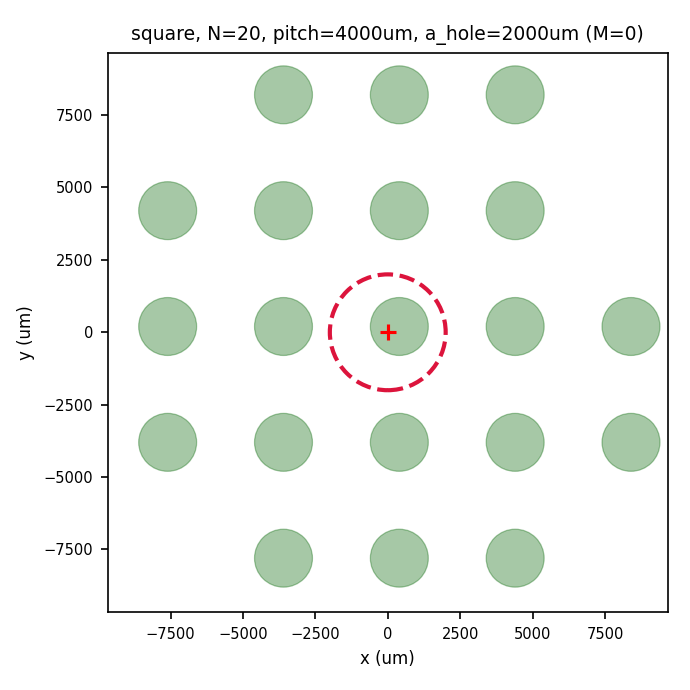
\includegraphics[width=\textwidth]{figures/GazeWeighted_M0_square_pitch4000_N20_a2000um.png}\end{minipage}
\begin{minipage}{0.32\textwidth}\centering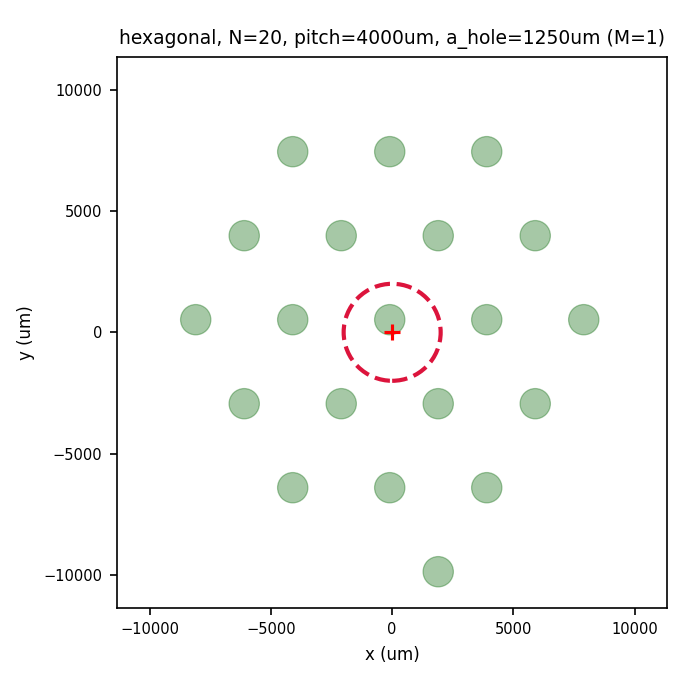
\includegraphics[width=\textwidth]{figures/GazeWeighted_M1_hexagonal_pitch4000_N20_a1250um.png}\end{minipage}
\begin{minipage}{0.32\textwidth}\centering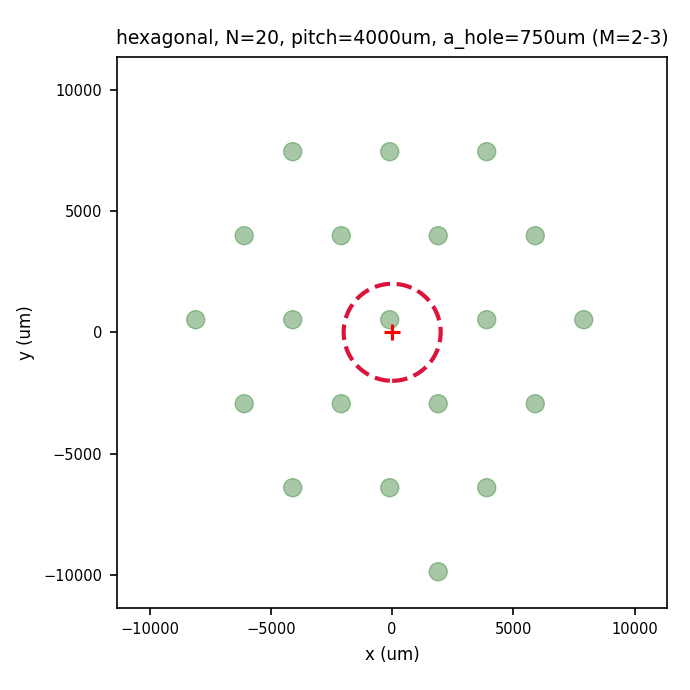
\includegraphics[width=\textwidth]{figures/GazeWeighted_M2-3_hexagonal_pitch4000_N20_a750um.png}\end{minipage}

\vspace{4pt}
\begin{minipage}{0.32\textwidth}\centering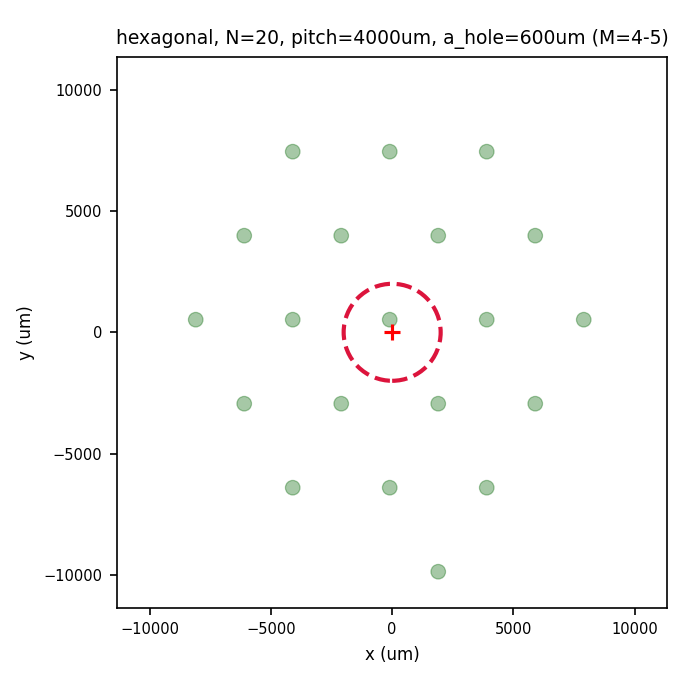
\includegraphics[width=\textwidth]{figures/GazeWeighted_M4-5_hexagonal_pitch4000_N20_a600um.png}\end{minipage}
\begin{minipage}{0.32\textwidth}\centering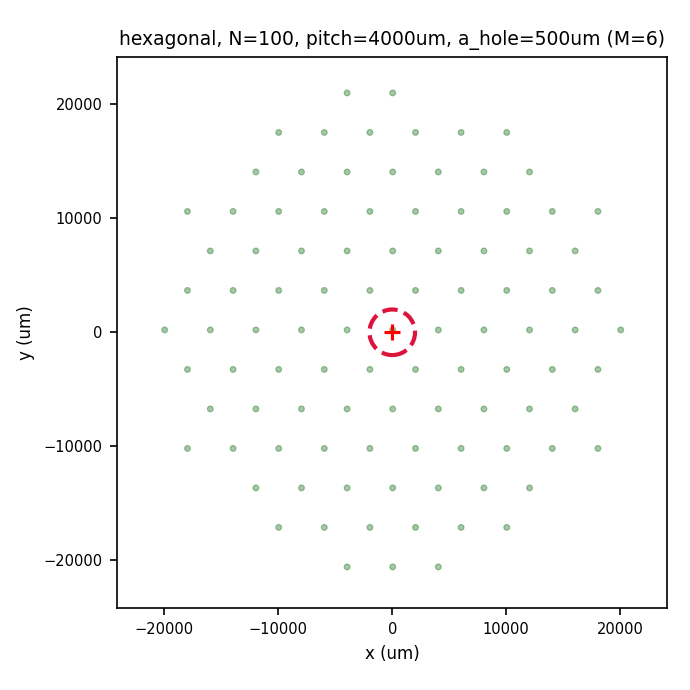
\includegraphics[width=\textwidth]{figures/GazeWeighted_M6_hexagonal_pitch4000_N100_a500um.png}\end{minipage}
\begin{minipage}{0.32\textwidth}\centering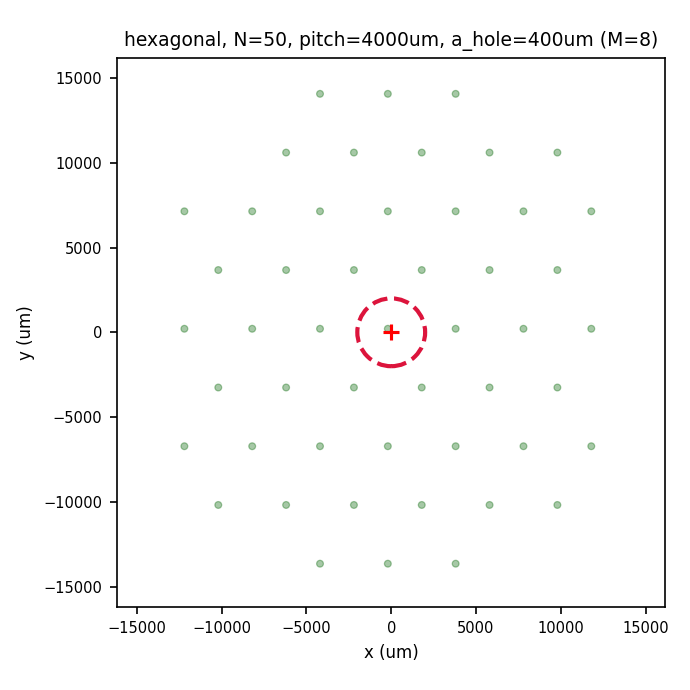
\includegraphics[width=\textwidth]{figures/GazeWeighted_M8_hexagonal_pitch4000_N50_a400um.png}\end{minipage}

\vspace{4pt}
\begin{minipage}{0.32\textwidth}\centering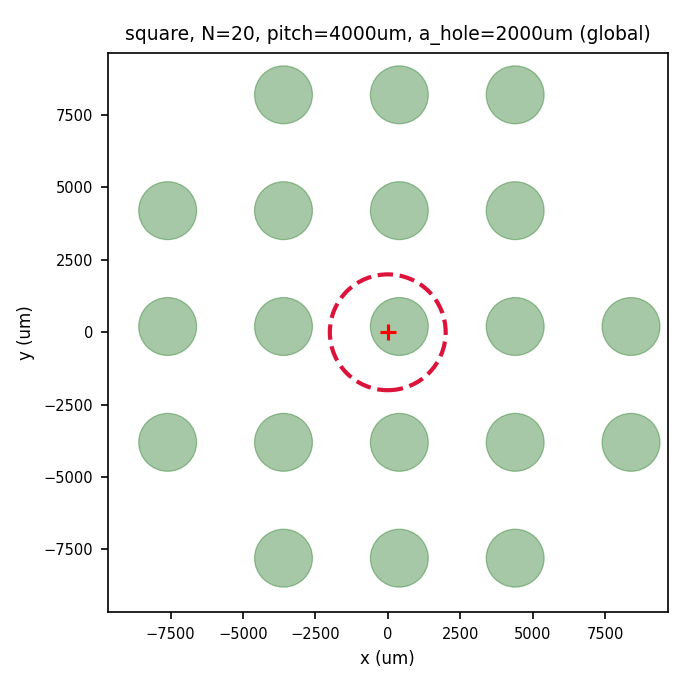
\includegraphics[width=\textwidth]{figures/GazeWeighted_Global_square_pitch4000_N20_a2000um.png}\end{minipage}
\caption{Real hole layouts, Model~B (gaze-weighted, current primary standard) winning
design per $M$ -- $M=0,1,2\text{--}3,4\text{--}5,6,8$D and the global (worst-case-across-$M$)
scope. Source:
\texttt{Array\_Design/array\_geometry\_lab/Design Visualisation/pngs\_for\_presentation/}
\texttt{GazeWeighted\_*.png}, all 7 files mtime 2026-09-17 21:32 (verified via
\texttt{stat}).}
\label{fig:layout-gaze-weighted}
\end{figure}

\begin{figure}[htbp]
\centering
\begin{minipage}{0.32\textwidth}\centering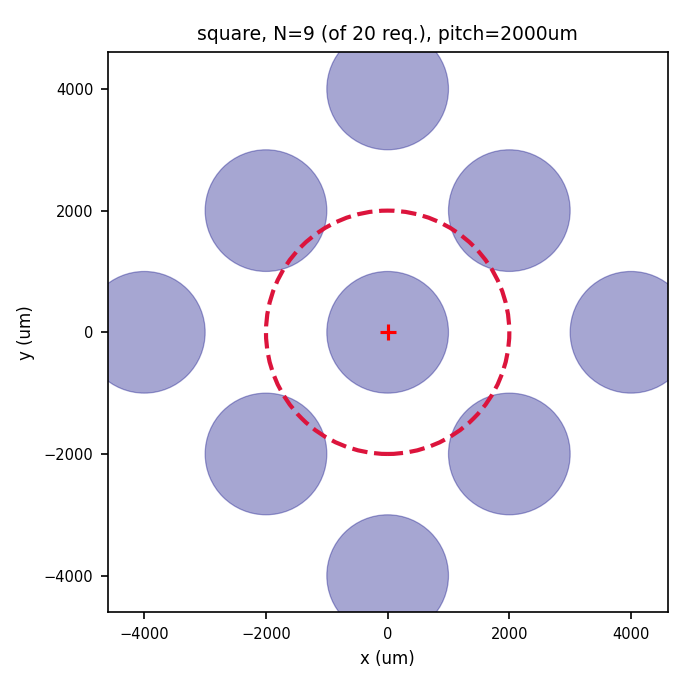
\includegraphics[width=\textwidth]{figures/WorstCase_M0_ringOffsetConcentric_rs1000_N11_a2000um.png}\end{minipage}
\begin{minipage}{0.32\textwidth}\centering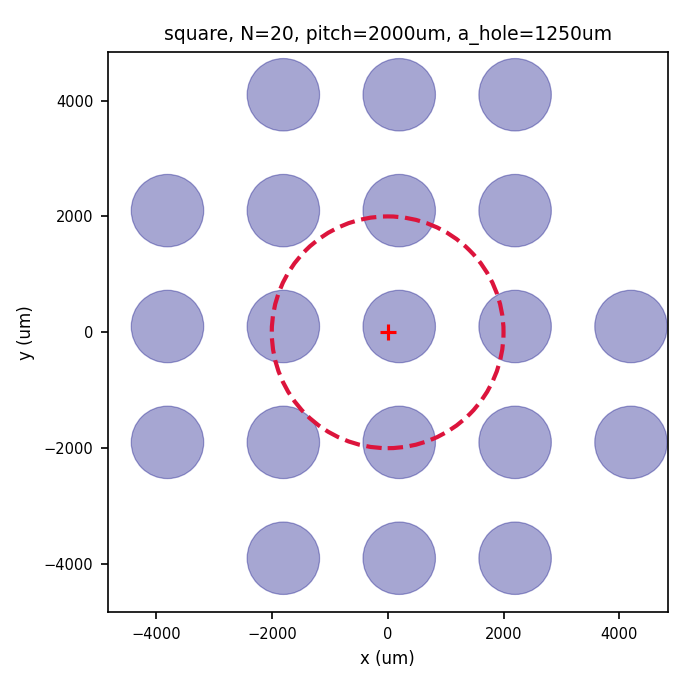
\includegraphics[width=\textwidth]{figures/WorstCase_M1_square_pitch2000_N20_a1250um.png}\end{minipage}
\begin{minipage}{0.32\textwidth}\centering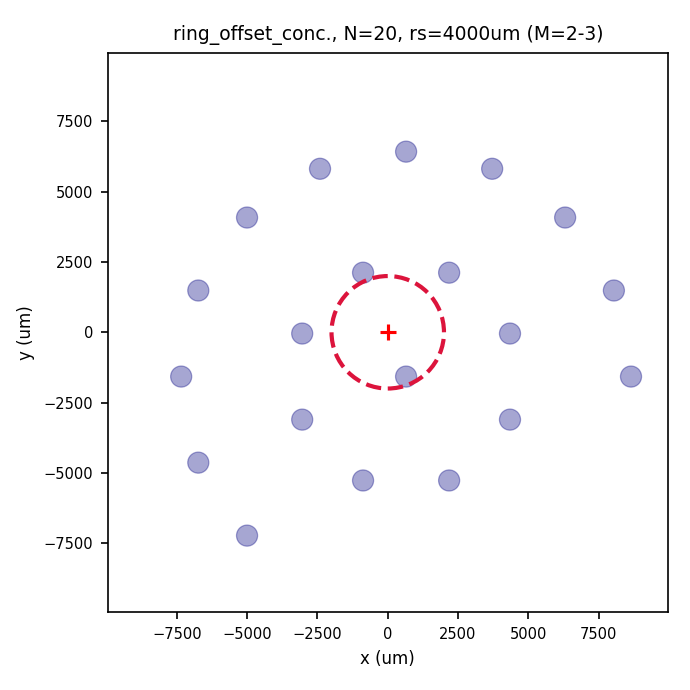
\includegraphics[width=\textwidth]{figures/WorstCase_M2-3_ringOffsetConcentric_rs4000_N20_a750um.png}\end{minipage}

\vspace{4pt}
\begin{minipage}{0.32\textwidth}\centering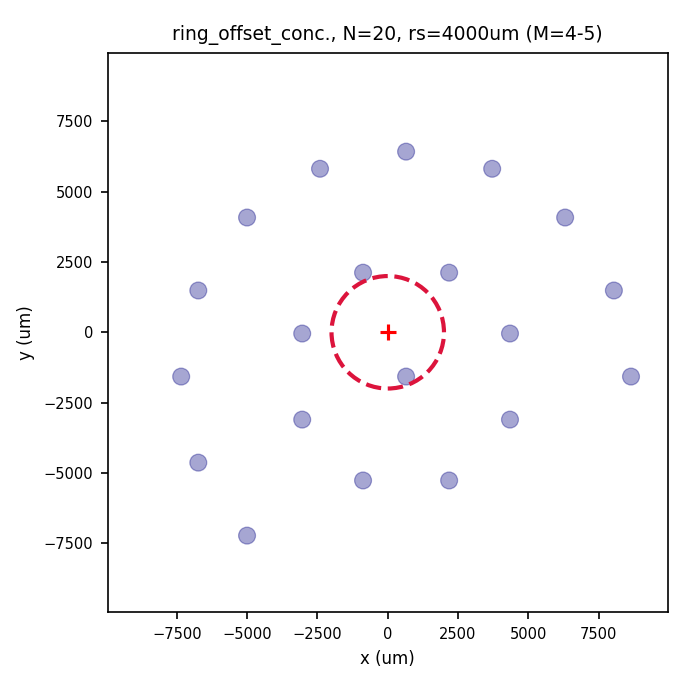
\includegraphics[width=\textwidth]{figures/WorstCase_M4-5_ringOffsetConcentric_rs4000_N20_a600um.png}\end{minipage}
\begin{minipage}{0.32\textwidth}\centering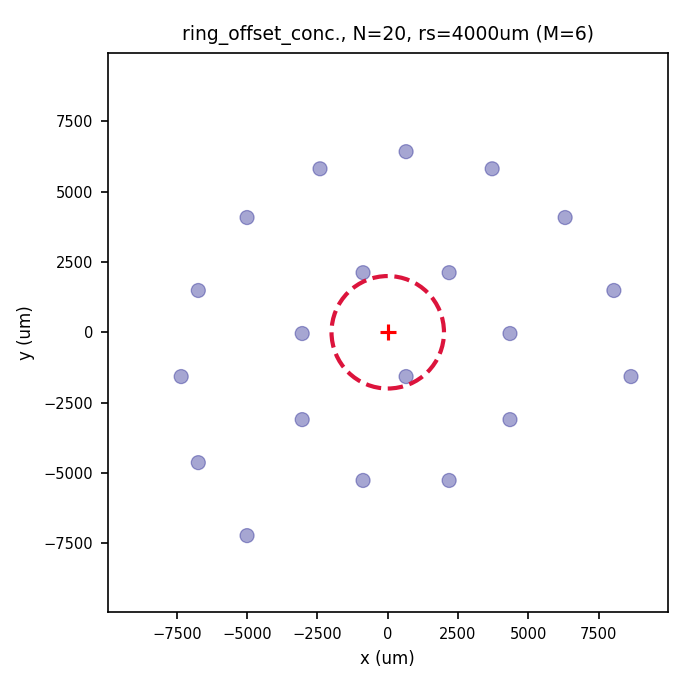
\includegraphics[width=\textwidth]{figures/WorstCase_M6_ringOffsetConcentric_rs4000_N20_a500um.png}\end{minipage}
\begin{minipage}{0.32\textwidth}\centering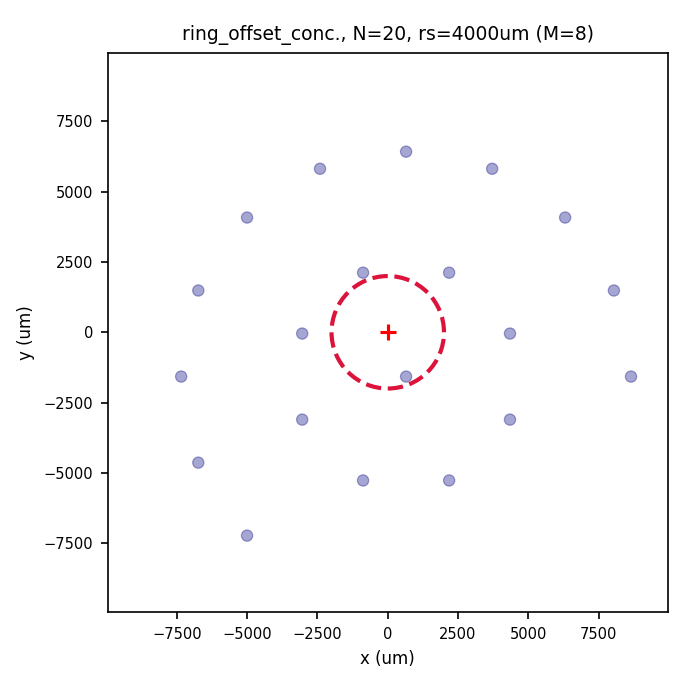
\includegraphics[width=\textwidth]{figures/WorstCase_M8_ringOffsetConcentric_rs4000_N20_a400um.png}\end{minipage}

\vspace{4pt}
\begin{minipage}{0.32\textwidth}\centering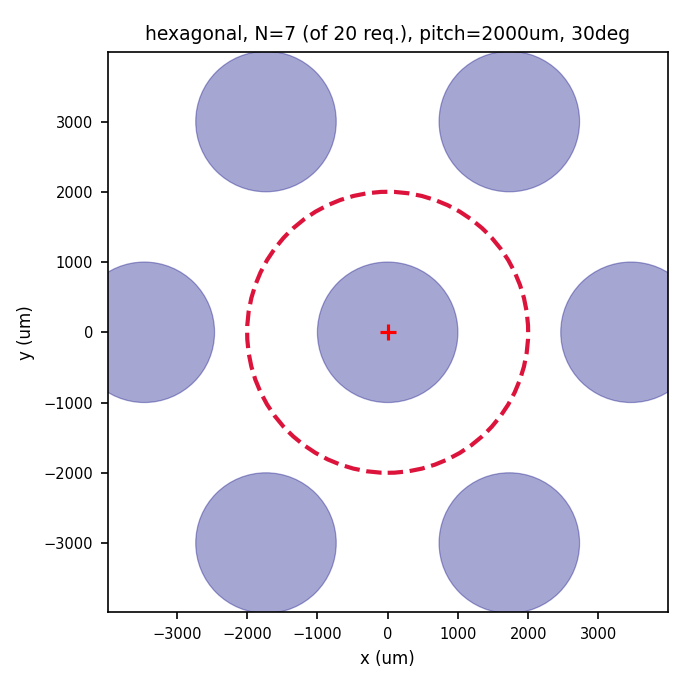
\includegraphics[width=\textwidth]{figures/WorstCase_Global_hexagonal_pitch2000_rot30_N7_a2000um.png}\end{minipage}
\caption{Real hole layouts, Model~A (single-axis worst-case gate, superseded primary
standard, Section~\ref{sec:model-a-limitation}) winning design per $M$. Note the family
mix (ring\_offset\_concentric dominates here, versus hexagonal's dominance in
Figure~\ref{fig:layout-gaze-weighted}) -- the visible consequence of the methodology
change documented in Chapter~\ref{ch:model-b}. Source: same folder as above,
\texttt{WorstCase\_*.png}, all 7 files mtime 2026-09-17 21:32.}
\label{fig:layout-worst-case}
\end{figure}

\section{Simulated retinal light-intensity distribution}
\label{sec:array-exp1}
A real ASM wave-optics simulation of the retinal intensity pattern each fabricated
design would produce, at straight-ahead gaze, was computed directly from
\texttt{stage2\_fixed/phase2\_retina.py}'s own \texttt{run\_pipeline\_point} (the same
function underlying every acuity number in this paper, Section~\ref{sec:asm}) -- not a
schematic approximation. At $\varphi=0$, every real winning design has exactly one
active hole (Table, Section~\ref{sec:model-b-results}), so the retinal image is
identical to that of a standalone single pinhole of the design's own chosen aperture.

\begin{figure}[htbp]
\centering
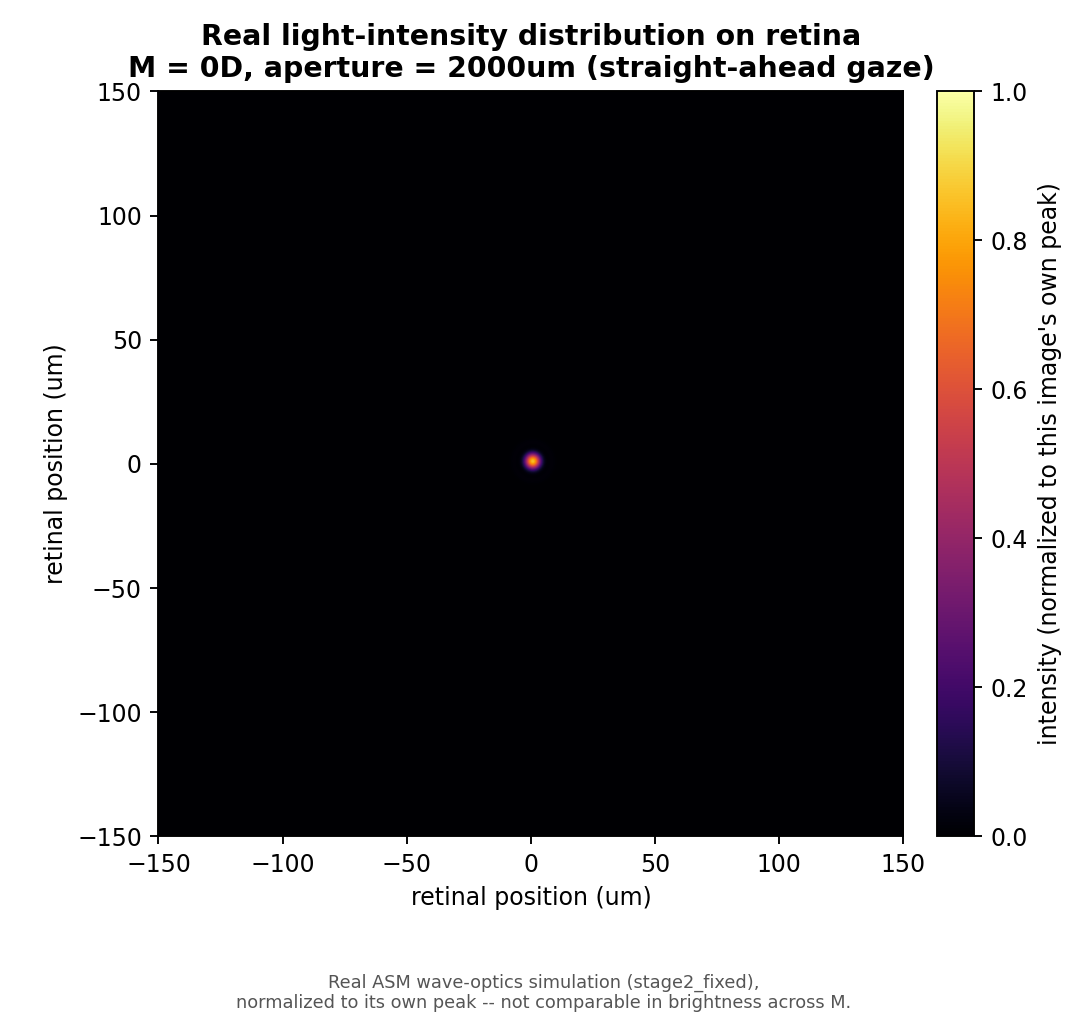
\includegraphics[width=0.30\textwidth]{figures/realistic_heatmap_M0.png}\hfill
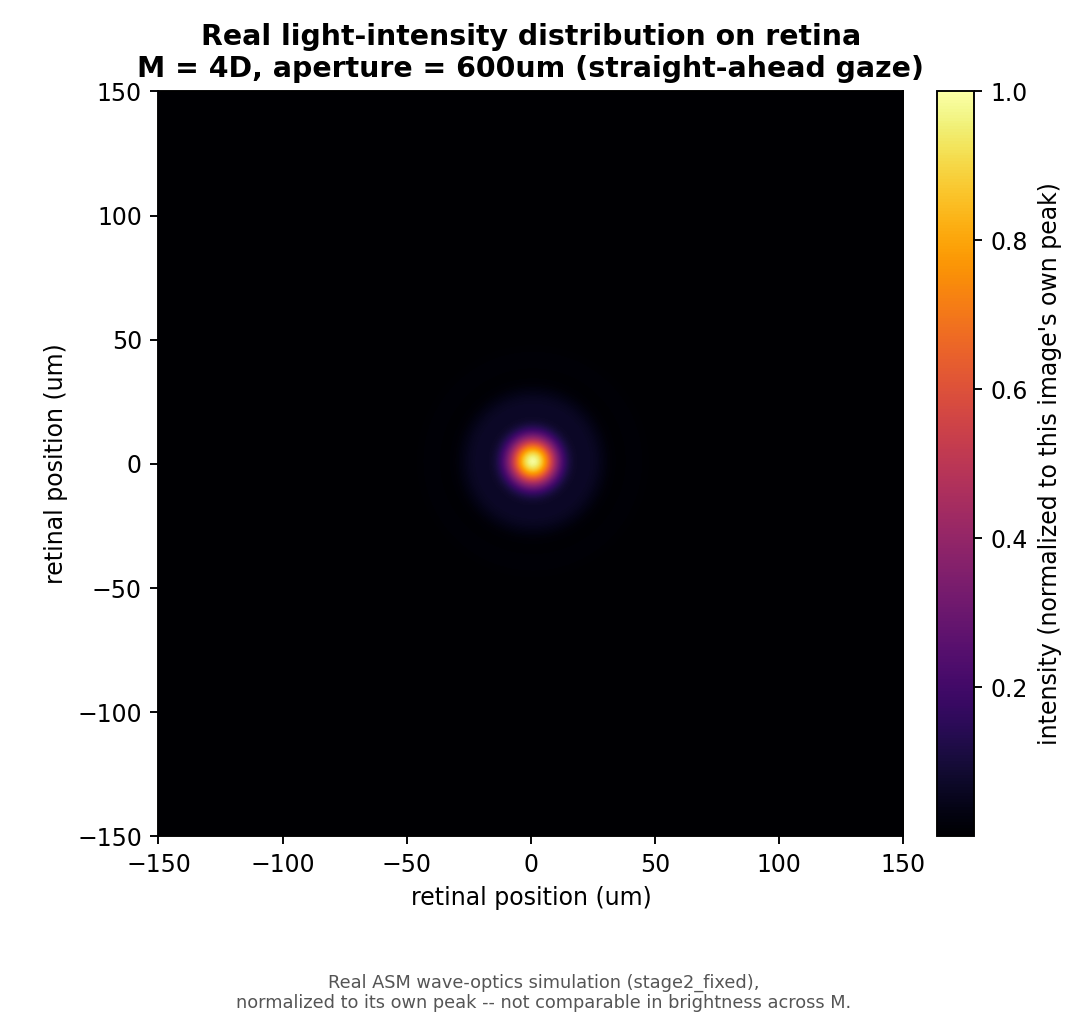
\includegraphics[width=0.30\textwidth]{figures/realistic_heatmap_M4.png}\hfill
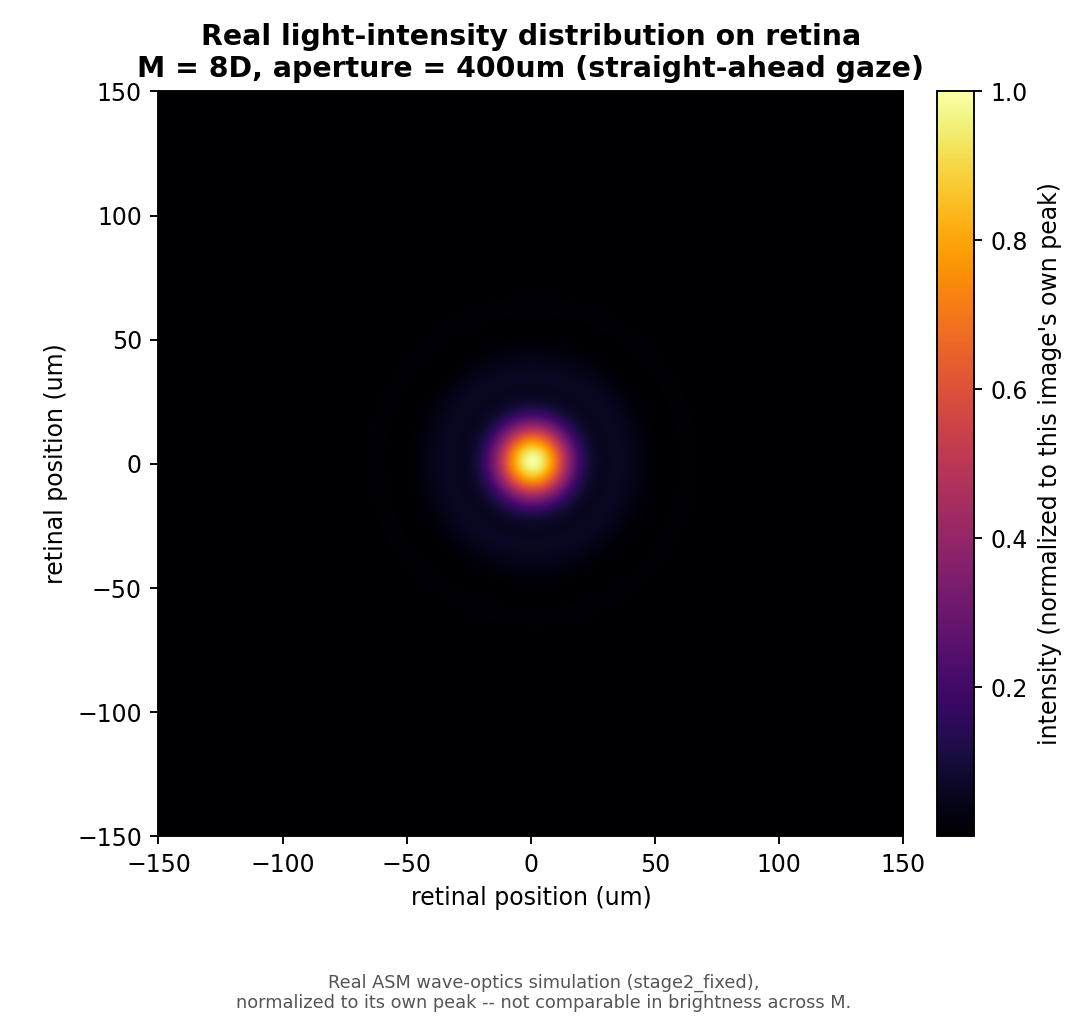
\includegraphics[width=0.30\textwidth]{figures/realistic_heatmap_M8.png}
\caption{Real, simulated retinal light-intensity distribution (straight-ahead gaze) at
$M=0,4,8$D, using each $M$'s own real \texttt{PRIMARY\_WINNER\_PER\_M} aperture (2000,
600, 400\,$\mu$m respectively). Computed directly from \texttt{stage2\_fixed}'s ASM
propagation, $N_{\mathrm{grid}}=4096$, identical parameters to the rest of this paper;
each panel normalized to its own peak intensity (absolute brightness is not
radiometrically comparable across panels without a source-power calibration this
project has not made; the blur \emph{shape} and relative \emph{size} growing from
$M=0$ to $M=8$ are real). Source: this analysis, direct call to
\texttt{stage2\_fixed.phase2\_retina.run\_pipeline\_point}; see Chapter~\ref{ch:provenance}.}
\label{fig:realistic-heatmaps}
\end{figure}

\section{A proposed physical validation rig}
\label{sec:proposed-rig}
A specific physical apparatus was designed (schematic: point source $\to$ rotating
pinhole-array insert $\to$ fixed $+20$D convex lens $\to$ a bare camera sensor (``mock
retina'') on a calibrated, Raspberry-Pi-3B+-driven linear rail) intended to measure the
real light-intensity distribution on a physical sensor as a function of simulated
myopic defocus (sensor axial displacement) and simulated gaze azimuth (array rotation).

\needsverify{As of this writing, this rig has NOT been built, and no physical
measurement data from it exists anywhere in this repository. This is stated explicitly
in this project's own animation/explainer material for the rig
(\texttt{Array\_Design/array\_geometry\_lab/proposed\_rig\_animation/}, which labels
every rendered frame ``THEORETICAL PREVIEW -- not measured sensor data''). It is
reported here as a specified, physically well-defined, but unexecuted proposal, not as
a completed experiment -- see also Section~\ref{sec:array-exp2} below and
Chapter~\ref{ch:limitations}.}

\section{Array-level clinical acuity trial}
\label{sec:array-exp2}
\begin{warnbox}{No array-level clinical trial data exists in this repository}
A search of the entire repository (every CSV for a per-subject or subject-count column,
every log file, every folder named with an experiment/clinical/trial-like pattern) found
\textbf{no} array-level, multi-subject clinical acuity trial data. What does exist is a
\emph{protocol specification} for a single-pinhole logMAR acuity measurement
(\texttt{Physics\_Guide/LOGMAR\_ACUITY\_PROTOCOL.tex}, Section~\ref{sec:logmar-protocol}),
which is explicitly designed to be extensible to a multi-subject trial but has, as far
as this repository's own files record, not yet been executed with real subjects for
either the single-aperture or the array-level case. This paper does not report, and
explicitly does not fabricate, any array-level clinical LogMAR results, deviation-vs-$M$
analysis, or subject count for this section. Any array-level clinical validation claim
made outside this document should be treated as unverified against the current
repository contents until a corresponding raw-data file is added and its provenance
recorded per Chapter~\ref{ch:provenance}.
\end{warnbox}

What this project \emph{does} have, and what Chapter~\ref{ch:model-comparison} reports
in full, is validation of the underlying single-aperture acuity model against
independently-published clinical data (Wang, 2009 \citep{wang2009}; Kim, 2017
\citep{kim2017}) -- real clinical LogMAR measurements, though not collected by this
project and not resolved per-myopia-power in the source studies. That comparison, and
its honest, unresolved statistical shortfall, is the closest this project currently has
to an array-relevant clinical acuity check, and is treated as such, not conflated with
a genuine array-specific clinical trial.

\chapter{Comparison to Reality}
\label{ch:model-comparison}

\section{Predicted acuity across all six evaluation models}
\label{sec:model-comparison-full}
Source: \texttt{Array\_Design/array\_geometry\_lab/predicted\_logmar\_analysis/predicted\_logmar\_wide\_by\_model.csv},
mtime 2026-09-28 10:09.

\begin{table}[htbp]
\centering
\begin{tabular}{cccccc}
\toprule
$M$ (D) & $a_{\mathrm{hole}}$ ($\mu$m) & Predicted LogMAR & MAR (arcmin) & Snellen \\
\midrule
0 & 2000 & $-0.357$ & 0.440 & 20/9 \\
1 & 1250 & $-0.120$ & 0.759 & 20/15 \\
2 & 750 & $+0.076$ & 1.190 & 20/24 \\
3 & 750 & $+0.112$ & 1.293 & 20/26 \\
4 & 600 & $+0.181$ & 1.516 & 20/30 \\
5 & 600 & $+0.240$ & 1.738 & 20/35 \\
6 & 500 & $+0.259$ & 1.813 & 20/36 \\
8 & 400 & $+0.331$ & 2.141 & 20/43 \\
\bottomrule
\end{tabular}
\caption{Predicted LogMAR is \emph{numerically identical} across all six live
evaluation models tested (worst-case gate/Model~A, ungated gaze-weighted, gated
gaze-weighted/Model~B, density-only Metric~1, and two effective-density variants) --
every model chooses the same acuity-optimal aperture per $M$ from
\texttt{new\_sweeps/per\_M\_optimum\_map.csv} (mtime 2026-09-13 00:11) before deciding
geometry, per Section~\ref{sec:model-comparison-table}.}
\label{tab:predicted-acuity}
\end{table}

\begin{figure}[htbp]
\centering
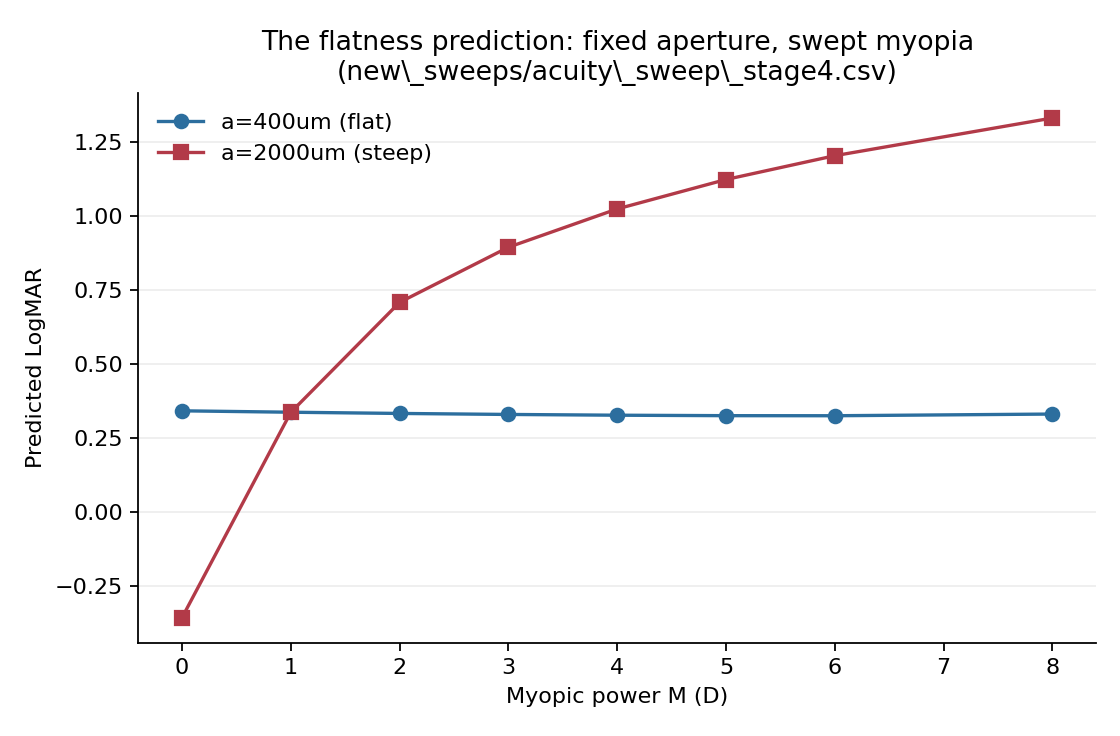
\includegraphics[width=0.75\textwidth]{figures/flatness_prediction.png}
\caption{The flatness prediction (Section~\ref{sec:flatness-prediction}): predicted
LogMAR vs.\ myopia power at fixed aperture. Recomputed directly from the current
\texttt{new\_sweeps/acuity\_sweep\_stage4.csv} (mtime 2026-09-13 00:11) for this paper;
spread at $a=400\,\mu$m is $0.0166$ LogMAR across the full 8-dioptre range, against
$1.687$ LogMAR at $a=2000\,\mu$m -- a $102\times$ difference.}
\label{fig:flatness}
\end{figure}

\section{The flatness prediction}
\label{sec:flatness-prediction}
Holding aperture fixed at $400\,\mu$m and sweeping myopia $M=0$ to $8$D, predicted
LogMAR varies by only $0.0166$ across the full range (source: this analysis, direct
computation from \texttt{new\_sweeps/acuity\_sweep\_stage4.csv}, current file) --
roughly a twentieth of one acuity-chart line, well below the $\pm0.1$ LogMAR
repeatability of human acuity testing. At this aperture, the \emph{aperture}, not the
wearer's own refractive error, sets predicted acuity. At $a=2000\,\mu$m the same sweep
spans $-0.357$ ($M=0$) to $+1.330$ ($M=8$), a spread $102\times$ larger. This is the
project's strongest, most falsifiable single prediction: it requires no knowledge of
any subject's exact prescription, only a qualitative ranking of myopia severity,
because the predicted \emph{signature} is a flat line for a well-chosen small-aperture
pinhole condition against a steep one for the unaided (or large-aperture) eye.

\section{External validation against real clinical data}
\label{sec:external-validation}
Two independently-published, directly-verified clinical datasets provide the only real
(non-simulated) LogMAR validation available anywhere in this project: Wang (2009)
\citep{wang2009} (5 apertures, $M=\{0,2,5\}$D tested, observed LogMAR
$0.28/0.31/1.00/0.40/0.50$ -- aperture-indexed only, the source paper reports
\textbf{no per-myopia-power breakdown at all}, so the same 5 observed values are
necessarily reused at every tested $M$, a real limitation of the source data, not an
approximation introduced by this project), and Kim (2017) \citep{kim2017} (single
$900\,\mu$m anchor, $N=36$, mean $M=-2.7\pm2.3$D, observed LogMAR $0.20\pm0.21$).

\subsection{A stale-data correction, made during this project's own development}
\label{sec:stale-wang}
\texttt{stage4\_human\_vision/outputs/validation\_predicted\_vs\_observed.csv} (mtime
2026-07-29 16:35) predates the 2026-08-06 \texttt{stage2/}$\to$\texttt{stage2\_fixed/}
optics fix (Section~\ref{sec:bug-shadowing}) by 8 days, and was found to give
materially different numbers from a fresh re-run with current code (e.g.\ aperture
$750\,\mu$m, $M=2$D: $0.076$ current vs.\ $1.010$ in the stale file). A corrected
``postfix'' re-run already existed
(\texttt{wang2009\_validation\_postfix\_predicted.csv}, mtime 2026-08-06 14:43) but its
own downstream calibration step had never been re-applied; this gap is closed in this
paper's own analysis (\texttt{predicted\_logmar\_analysis/wang2009\_calibration\_pooled\_stats\_postfix.csv},
computed 2026-09-28, using \texttt{stage4\_human\_vision/calibration.py}'s existing,
unmodified fitting functions). \textbf{Every number in this section uses the corrected,
post-fix data.}

\begin{table}[htbp]
\centering
\begin{tabular}{lccccc}
\toprule
Comparison & $n$ & $R^2$ & Pearson $r$ & $p$ & $R^2{>}0$ and $p{<}0.05$? \\
\midrule
$M=0$D, raw model & 5 & $-4.80$ & $-0.375$ & $0.533$ & FAIL \\
$M=2$D, raw model & 5 & $-1.41$ & $-0.180$ & $0.772$ & FAIL \\
$M=5$D, raw model & 5 & $-0.68$ & $+0.426$ & $0.474$ & FAIL \\
Pooled ($n{=}15$), raw, uncalibrated & 15 & $-2.30$ & $+0.019$ & $0.947$ & FAIL \\
Pooled, affine-calibrated, in-sample & 15 & $0.0003$ & $+0.019$ & $0.947$ & FAIL \\
Pooled, affine-calibrated, leave-one-out & 15 & $-0.31$ & $-0.928$ & $0.0000$ & FAIL \\
\bottomrule
\end{tabular}
\caption{The model fails the stated bar ($R^2>0$ AND $p<0.05$) at every single
comparison, before and after the 2026-08-06 optics fix, and before and after affine
calibration. Source: \texttt{stage4\_human\_vision/outputs/wang2009\_validation\_postfix\_stats.csv}
(per-$M$ rows) and \texttt{predicted\_logmar\_analysis/wang2009\_calibration\_pooled\_stats\_postfix.csv}
(pooled rows), both verified read directly, 2026-09-28.}
\label{tab:r2-status}
\end{table}

\begin{keybox}{The fix helped, measurably, without fixing the underlying failure}
Pooled raw $R^2$ improved from $-4.98$ (pre-fix) to $-2.30$ (post-fix) -- a real,
substantial narrowing of the gap, not a rounding-level shift -- but the model still
fails the significance bar at every single tested condition, before and after. In-sample
affine calibration gives essentially \emph{zero} explanatory power post-fix ($R^2=0.0003$,
down from $+0.132$ pre-fix), meaning the earlier apparent calibration benefit was itself
partly an artifact of the since-corrected optics bug, not a real effect of the
calibration procedure. This is reported as-is: neither ``still fails, nothing changed''
nor ``now passes,'' but the specific, quantified middle case that a real, targeted
optics fix measurably improved without resolving the underlying shortfall.
\end{keybox}

\begin{figure}[htbp]
\centering
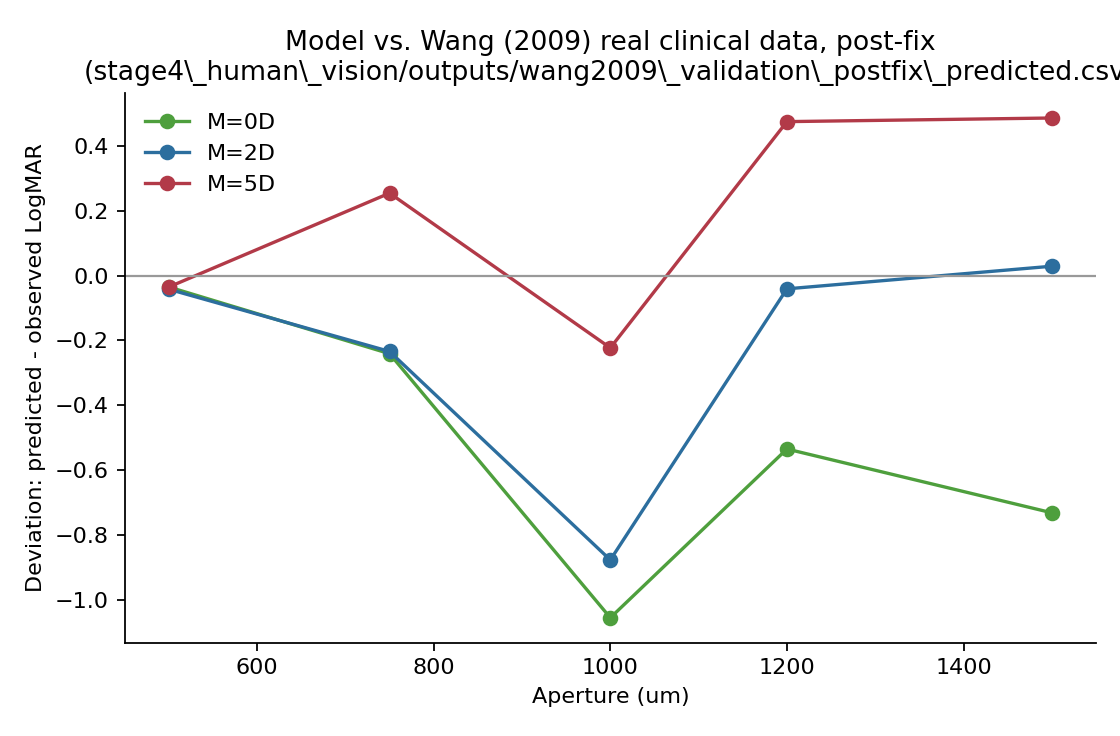
\includegraphics[width=0.75\textwidth]{figures/wang2009_deviation.png}
\caption{Model deviation (predicted $-$ observed LogMAR) vs.\ aperture, post-fix, all
three tested myopia powers. Deviation sign is not constant across the aperture range --
the model is measurably optimistic (predicts better vision than observed) at small
apertures and pessimistic at some large-aperture/high-$M$ combinations, i.e.\ this is
not a single universal bias. Source: this analysis, from
\texttt{wang2009\_validation\_postfix\_predicted.csv}.}
\label{fig:wang-deviation}
\end{figure}

\subsection{At the specific apertures this project's own array designs actually use}
Restricting the comparison to the exact (aperture, $M$) pairs the real array winners of
Chapter~\ref{ch:model-b} actually use (500 and 750\,$\mu$m, at $M=6$D and $M=2/3$D
respectively -- the only overlap between Wang's tested aperture set and this project's
own chosen apertures), the model is modestly-to-moderately \emph{optimistic}: deviation
$-0.234$ ($M=2$, $750\,\mu$m), $-0.198$ ($M=3$, $750\,\mu$m), $-0.022$ ($M=6$,
$500\,\mu$m) -- $0.2$--$2.3$ acuity-chart lines too favourable, direction consistent
across all three points (source: this analysis, from
\texttt{new\_sweeps/acuity\_sweep\_stage4.csv} cross-referenced against Wang's own
aperture-indexed observed values).

\subsection{A second real anchor: Kim (2017)}
At $a=900\,\mu$m, $M=2.7$D (this study's own reported mean): predicted LogMAR
$=0.277$, observed $0.20\pm0.21$ ($n=36$) -- deviation $+0.077$, \textbf{pessimistic},
the \emph{opposite} sign from the 500/750\,$\mu$m points above, and within one standard
deviation of the real data's own spread. This anchor was already present in this
project's own vetted literature (\texttt{stage4\_human\_vision/literature.py}, flagged
``USABLE as one additional real anchor'') but had never actually been run through the
model before this paper's own analysis. \textbf{Key honest takeaway}: the model's error
is not a single universal ``always optimistic by $X$'' bias -- both direction and
magnitude depend on the specific aperture/myopia-power region.

\subsection{A note on search-derived claims}
\label{sec:search-honesty}
A live search for additional external pinhole-aperture-vs-acuity datasets, undertaken
during this project's own development, reproduced -- verbatim -- a specific numeric
claim (``0.17 LogMAR at up to 5.5D, 1.16 LogMAR at 7--11D'') that this project's own
literature review had \emph{already} investigated and marked REJECTED after reading the
purported primary source directly and confirming those numbers do not appear anywhere
in it \citep{neuroquantology2022rejected}. This is documented here as direct, concrete
evidence that AI-search-summary claims on this specific topic are not reliable without
independent primary-source verification -- a finding this project treats as a
methodological caution for its own future literature work, not merely an isolated
incident.

\chapter{Errors Identified and Corrected}
\label{ch:errors}

This chapter is a required, explicit part of this paper, not an appendix of
afterthoughts: four real implementation defects were found and corrected during this
project's own development, each with concrete before/after evidence. They are
documented here as worked case studies because the corrections are themselves part of
the project's contribution.

\section{The single-FFT defocus-plane bug}
\label{sec:bug-fft}
\textbf{The trap.} A naive single-lens imaging simulation -- clip the field to the
pupil, multiply by the lens's quadratic phase, take one Fourier transform -- computes
the field at \emph{the lens's own back focal plane}. For a healthy (emmetropic) eye
that plane coincides with the retina, and the naive approach is correct by coincidence.
For a myopic eye the retina is, by definition, \emph{not} at that focal plane -- that
mismatch is the definition of myopia -- and a single FFT silently computes the field at
the wrong physical location (source:
\texttt{Physics\_Guide/PHYSICS\_AND\_FABRICATION\_GUIDE.tex}, lines 160--165, verified
read directly).

\begin{warnbox}{What the bug would have produced, had it shipped}
A beautiful, sharp Airy pattern computed at the eye's true focal point -- the one plane
in the whole system where defocus blur is, by construction, exactly zero. The output
would model a perfectly-corrected eye and report it as myopic. The plot looks entirely
plausible; the physics is inverted.
\end{warnbox}

\textbf{The fix.} Full angular-spectrum propagation (Equation~\ref{eq:asm}) over the
\emph{actual} myopic axial distance $v_r=L_{\mathrm{ax}}(M)\ne f_{\mathrm{eye}}$, not a
single FFT assumed to land on the retina. This is the entire reason
Chapter~\ref{ch:single}'s pipeline uses ASM for both propagation stages rather than a
single closed-form transform, and is validated independently in
Section~\ref{sec:asm-validation}.

\section{The stage2/ vs.\ stage2\_fixed/ import-shadowing bug}
\label{sec:bug-shadowing}
\textbf{The bug.} \texttt{stage4\_human\_vision/pipeline.py} inserted the
\emph{deprecated} \texttt{stage2/} directory into \texttt{sys.path} and imported
\texttt{phase2\_retina} from there, not from \texttt{stage2\_fixed/}, despite living in
this project's own ``Stage 4'' directory specifically to sit on top of the corrected
Stage 2/3 pipeline. \texttt{stage2/phase2\_retina.py} independently carries the
lens-phase/retina-propagation wavelength bug: the eye's lens phase was applied using
the raw vacuum wavelength while the retina propagation used the vitreous's reduced
wavelength ($\lambda/n'$), under-applying the lens's converging phase by a factor of
$n'\approx1.336$ whenever \texttt{refractive\_index\_correction=True} (this project's
own default) -- shifting the field's true geometric focus away from where the retina is
actually evaluated, at \emph{every} myopia level and aperture \texttt{run\_stage4\_point}
was ever called with (source: \texttt{stage4\_human\_vision/RESULTS.md}, ``Re-run against
corrected optics,'' verified read directly, mtime 2026-08-06 14:43).

A second-order consequence: because \texttt{pipeline.py}'s import runs first whenever
anything under \texttt{stage4\_human\_vision} is imported (via its own
\texttt{\_\_init\_\_.py}), it silently \emph{shadowed} an entirely separate module's
(\texttt{R7acuity}'s) own, correctly-targeted \texttt{stage2\_fixed/} import too, via
Python's bare-module-name caching in \texttt{sys.modules} -- one shared root cause
independently corrupted two different downstream models' validation results, each
reported independently in that model's own \texttt{RESULTS.md}.

\textbf{The fix.} \texttt{pipeline.py}'s \texttt{sys.path} insertion was repointed at
\texttt{stage2\_fixed/}; \texttt{stage3\_human\_vision/metrics.py} had the identical
defect and was fixed the same way. Verified before fixing
(\texttt{sys.modules['phase2\_retina'].\_\_file\_\_}) that the shadowing reproduced, and
after fixing that it resolves to \texttt{stage2\_fixed/phase2\_retina.py}.

\begin{center}
\begin{tabular}{cccc}
\toprule
$M$ (D) & $R^2$ (pre-fix) & $R^2$ (post-fix) & Improvement \\
\midrule
0 & $-6.39$ & $-4.80$ & $+1.6$ \\
2 & $-4.98$ & $-1.41$ & $+3.6$ \\
5 & $-2.84$ & $-0.68$ & $+2.2$ \\
\bottomrule
\end{tabular}
\end{center}
\textbf{Verdict: still fails the $R^2{>}0,\,p{<}0.05$ bar at every $M$ -- but a real,
substantial, and consistent improvement in the right direction at every $M$ tested.}
Pearson $r$ \emph{worsened} or flipped sign at $M=0$ and $M=2$ even as $R^2$ improved,
because $R^2$ penalizes systematic bias/offset (every predicted point sitting above the
diagonal, pre-fix) while Pearson $r$ measures only rank correlation -- the corrected
optics reduced the bias enough to improve $R^2$ while disturbing whatever weak
rank-ordering existed before. Reported as-is, not smoothed over by selecting whichever
statistic looks more favourable (source:
\texttt{stage4\_human\_vision/RESULTS.md}, verified read directly).

\subsection{A follow-on staleness discovery}
A specific downstream consequence of this fix was found only during this paper's own
preparation: \texttt{validation\_predicted\_vs\_observed.csv} (dated 2026-07-29,
8 days \emph{before} the 2026-08-06 fix above) was still being read by later analysis as
if it were current, though a correctly-dated ``postfix'' re-run already existed
alongside it. Full detail in Section~\ref{sec:stale-wang}; this is documented as its own
sub-instance of the general staleness pattern this project has now encountered twice
(the other being Section~\ref{sec:bug-gridN}).

\section{Model A's single-axis gaze limitation}
\label{sec:bug-single-axis}
Not a coding defect in the sense of the other three entries in this chapter, but a
genuine, acknowledged \emph{modelling} limitation with a real, concrete failure
instance: Model~A's vignetting evaluation samples gaze along one fixed axis only. A
specific \texttt{concentric\_centered} candidate that outperformed the then-current
winner everywhere inside $15^\circ$ was found to fail catastrophically -- a complete
blackout -- in the $20$--$25^\circ$ gaze range at an azimuth Model~A's single axis never
tested (source: \texttt{CENTERED\_CONCENTRIC\_COMPARISON.md}, 2026-08-17, verified
present). This is the concrete motivating case for building Model~B's full-azimuth
sampling (Section~\ref{sec:model-b-method}); see Section~\ref{sec:model-a-limitation}
for the mechanism and Section~\ref{sec:hex-intuition} for the geometric reason
hexagonal packing is comparatively resistant to it.

\section{The grid-resolution ($N_{\mathrm{grid}}$) staleness bug}
\label{sec:bug-gridN}
\textbf{The bug.} \texttt{stage4\_human\_vision/pipeline.py}'s \texttt{run\_stage4\_point}
defaults to $N_{\mathrm{grid}}=2048$. At this resolution, computed blur radii for large
apertures ($\gtrsim1500$--$2000\,\mu$m) come out approximately $2\times$ too large
compared to the converged value at $N_{\mathrm{grid}}=4096$ -- a numerical
under-resolution artifact (Section~\ref{sec:gridN}). \texttt{run\_blur\_sweep.py} was
fixed on 2026-08-16; \texttt{run\_acuity\_sweep.py} called the same underlying function
but was not updated to match until 2026-09-12/13, leaving nearly a month of
acuity-model output computed at the stale resolution.

\textbf{Blast-radius accounting.} Every file derived from the stale
\texttt{acuity\_sweep\_stage4.csv} was identified and regenerated:
\texttt{table1\_optimum\_summary.csv} (subsequently superseded entirely by
\texttt{per\_M\_optimum\_map.csv}), \texttt{per\_M\_optimum\_map.csv} itself, and every
figure derived from either. The entire downstream \texttt{array\_geometry\_lab}
evaluation pipeline was re-run in full rather than assuming only the directly-affected
files needed attention.

\textbf{Fix verified, not merely applied.} Because array hole \emph{geometry} is
generated deterministically from spacing parameters alone, independent of the acuity
model entirely, fabrication package outputs (hole-coordinate CSVs, mask SVGs) were
explicitly diffed pre- and post-fix and confirmed \textbf{byte-identical}
(Section~\ref{sec:fabrication}) -- the fix changed predicted acuity numbers, not
fabricated geometry, and this was checked rather than assumed.

\section{A related, lower-priority finding, disclosed for completeness}
\label{sec:bug-dashboard}
\texttt{master\_dashboard/wrappers.py}'s \texttt{sweep\_stage4\_acuity} also omits
$N_{\mathrm{grid}}$ (defaulting to $2048$) at its own call to
\texttt{run\_stage4\_point}. Unlike the three entries above, this function is an
interactive-dashboard-only code path: no committed, reported result file in this
project currently depends on its output. Flagged here for completeness and future
awareness, not treated as a fifth confirmed-impactful bug.

\chapter{Discussion}
\label{ch:discussion}

Returning to the problem statement (Chapter~\ref{ch:intro}): this project set out to
determine whether an array of small apertures can substitute for a corrective lens over
a useful field of view, and to characterize the trade-offs involved. The evidence
assembled here supports a qualified yes, with the trade-offs now quantified rather than
asserted.

\textbf{Single-aperture optics} (Chapter~\ref{ch:single}) establish that the stenopeic
effect is real and substantial (Section~\ref{sec:exp3}: a $15$--$18\times$ reduction in
defocus-growth rate, measured photographically, not merely predicted), and that an
exact wave-optics treatment is necessary, not a convenience: the closed-form RSS
approximation this project also implements diverges from the exact result by 64.8\% on
average, and a specific naive-FFT implementation trap (Section~\ref{sec:bug-fft}) would
have silently inverted the physics of myopic defocus entirely had it shipped
uncorrected.

\textbf{Array-level optics} (Chapter~\ref{ch:array-theory}) show that extending a single
aperture to an array introduces two new failure modes -- ghosting and blinding -- with
no single-aperture analogue, and that a naive per-aperture margin criterion for
ghosting is not merely imprecise but was shown, via the Barten CSF correction
(Section~\ref{sec:barten}), to reclassify the \emph{entire} tested dense-pitch range
from ``safe'' to ``danger zone.'' The harmonic-series extension
(Section~\ref{sec:harmonic}) further shows that even a corrected fundamental-frequency
analysis can underestimate real risk by over $4\times$ by missing the worst-case
harmonic.

\textbf{The two evaluation models} (Chapters~\ref{ch:model-a}--\ref{ch:model-b}) are not
in conflict: Model~B generalizes Model~A by removing its single-axis assumption, and
the fact that removing that assumption changed the outcome -- surfacing a real
blackout failure mode Model~A's own structural-safety guarantee had missed
(Section~\ref{sec:bug-single-axis}) -- is direct evidence the generalization mattered,
not merely a theoretical nicety. That hexagonal packing wins under the more rigorous
model is explained, not merely observed, by a first-principles symmetry argument
(Section~\ref{sec:hex-intuition}) grounded in the crystallographic restriction theorem,
and demonstrated with real, matched-spacing geometry and real, already-computed safety
data (Figures~\ref{fig:geom-structure}--\ref{fig:geom-consequence}).

\textbf{External validation} (Chapter~\ref{ch:model-comparison}) is this project's most
honestly limited result: the acuity model, in its raw form, fails a formal $R^2>0$
significance bar against every real clinical comparison available, both before and
after a genuine, verified optics fix that measurably narrowed (but did not close) the
gap. This paper does not claim the model is externally validated; it claims the model
is \emph{physically grounded}, internally self-consistent (Section~\ref{sec:asm-validation}),
improved measurably when a real defect was corrected (Section~\ref{sec:bug-shadowing}),
and its remaining discrepancy against real data is reported with the exact statistics,
not glossed over.

\chapter{Limitations}
\label{ch:limitations}

Stated plainly, in the order they matter for interpreting this project's results:

\begin{enumerate}
\item \textbf{External validation fails a formal significance bar.} Every tested
comparison against real clinical data (Wang 2009, Section~\ref{sec:external-validation})
gives $R^2\le0$; a genuine optics fix narrowed but did not close this gap
(Section~\ref{sec:bug-shadowing}). This is the single most important limitation of this
project's quantitative claims.
\item \textbf{Deviation from reality is not a single, constant bias, and its magnitude
is not shown to grow monotonically with any one variable.} Model error is optimistic at
some (aperture, $M$) combinations and pessimistic at others
(Section~\ref{sec:external-validation}); this project has not identified a single
scalar predictor of when the model will be more or less accurate.
\item \textbf{Both external clinical datasets used real, but not per-subject-resolved,
data.} Wang (2009)'s summary table reports acuity vs.\ aperture only, with no
per-myopia-power breakdown at all -- the same 5 observed values are necessarily reused
at every tested $M$ in this paper's own comparisons, a structural limitation of the
source data. Kim (2017) reports only group means and standard deviations, not
per-subject refractive error or acuity.
\item \textbf{Induced-defocus vs.\ native myopia.} Neither external dataset, nor this
project's own single-aperture experiments, distinguishes between subjects with genuine
native (axial) myopia and any induced-defocus condition; the axial myopia model
(Section~\ref{sec:reduced-eye}) assumes the former.
\item \textbf{Extrapolation beyond the validated gaze range.} Model~B's own gaze-time
weighting includes one bin at $27^\circ$, outside \texttt{vignetting\_overlap.py}'s
stated $\le25^\circ$ small-angle validity range (Section~\ref{sec:model-b-method}). The
formula does not diverge there, but every number that includes this bin is, by the
source module's own documentation, an extrapolation, not a validated result.
\item \textbf{Model A's single-axis legacy remains embedded in some reported numbers.}
Model~A (Chapter~\ref{ch:model-a}) is retained and reported in full, per this project's
own policy of not deleting superseded models, but its single-axis sampling convention
(Section~\ref{sec:model-a-limitation}) should not be read as an independent,
full-azimuth confirmation of any result -- only Model~B's numbers carry that property.
\item \textbf{No array-level clinical trial exists.} As documented in full in
Section~\ref{sec:array-exp2}, no multi-subject, array-level clinical LogMAR data exists
anywhere in this project's repository at the time of writing. The ``comparison to
reality'' this paper reports (Chapter~\ref{ch:model-comparison}) validates the
underlying \emph{single-aperture} acuity model only.
\item \textbf{The heuristic-vs-Barten CSF correction (Section~\ref{sec:barten}) has not
itself been re-run against the array-level Model~A/B evaluation pipeline.} It was
developed and validated in a separate, standalone sweep
(\texttt{Array\_Design/ghosting/}); this paper reports it as the theoretically correct
ghosting-perceptibility criterion but the live \texttt{gates.py}/Model~A and Model~B
pipelines reported in Chapters~\ref{ch:model-a}--\ref{ch:model-b} use the
active-hole-fraction/geometric-overlap criterion (Section~\ref{sec:vignetting}), not
the Barten-CSF three-regime criterion directly. \needsverify{Whether and how the
Barten-corrected ghosting classification of Section~\ref{sec:barten} has been, or
should be, integrated into the live \texttt{gates.py} ghost-safety gate was not
resolved during this paper's preparation and is flagged here rather than assumed either
way.}
\item \textbf{Reduced-eye model simplifications, stated explicitly rather than hidden.}
No anatomically-separate cornea/lens power split; no higher-order aberrations (only
pure quadratic defocus phase); no Stiles--Crawford directional pupil apodization in the
core PSF calculation (though a separate Stiles--Crawford term is applied elsewhere, in
\texttt{stage4\_human\_vision/csf.py}'s own retinal-illuminance calculation); no
longitudinal chromatic aberration (one fixed wavelength per run, not a dispersion
model); binary hard-edged aperture masks, no finite membrane-thickness diffraction or
oblique-angle vignetting effects (source:
\texttt{stage2\_fixed/phase2\_retina.py}'s own module docstring, PHYSICS\_AUDIT.md
items E1/E4, verified present).
\label{sec:limitations-optics}
\item \textbf{The proposed physical validation rig (Section~\ref{sec:proposed-rig}) is
unbuilt.} Every number this paper reports for that apparatus is a theoretical preview
from the already-validated simulation pipeline, explicitly labelled as such in its own
source material, not a physical measurement.
\end{enumerate}

\chapter{Future Work}
\label{ch:future}

In priority order, following directly from the limitations of Chapter~\ref{ch:limitations}:

\begin{enumerate}
\item \textbf{Execute the single-pinhole LogMAR acuity protocol} already specified in
full (\texttt{Physics\_Guide/LOGMAR\_ACUITY\_PROTOCOL.tex}, Section~\ref{sec:logmar-protocol}),
recruiting subjects across a range of native myopia severity, recording every
per-subject raw measurement (not only group means) and any excluded subject with a
pre-registered reason -- specifically designed to test the flatness prediction
(Section~\ref{sec:flatness-prediction}), this project's strongest falsifiable claim.
\item \textbf{Build and run the proposed array-level validation rig}
(Section~\ref{sec:proposed-rig}): rotating pinhole-array insert, fixed $+20$D lens,
RPi-driven linear-rail bare-sensor mock retina. This would directly test the real,
simulated retinal-intensity predictions of Section~\ref{sec:array-exp1} and Model~B's
own gaze-weighted ghost/blind predictions (Chapter~\ref{ch:model-b}) against a real
optical measurement for the first time.
\item \textbf{Design and execute a genuine array-level, multi-subject clinical trial}
(the gap documented in Section~\ref{sec:array-exp2}), with per-subject refractive error
recorded (a limitation shared by every external dataset used in this paper's own
validation, Chapter~\ref{ch:limitations} items 3--4), specifically targeting the
deviation-vs-aperture and deviation-vs-$M$ questions Chapter~\ref{ch:model-comparison}
could only address with $n=16$ points borrowed from two unrelated published studies.
\item \textbf{Integrate the Barten-CSF three-regime ghosting criterion}
(Section~\ref{sec:barten}) directly into the live \texttt{gates.py} evaluation pipeline
used by Models A and B, resolving the open question flagged in Chapter~\ref{ch:limitations}
item 8, and re-run Chapters~\ref{ch:model-a}--\ref{ch:model-b}'s results under that
corrected criterion to check whether any current winner's classification changes.
\item \textbf{Extend Model~B's validated gaze range.} Either obtain or derive a
pupil-shift formula validated beyond $25^\circ$, or explicitly bound the influence of
the $27^\circ$ extrapolated bin (currently 0.58\% of total gaze-time weight) on every
reported result, so its contribution can be reported as a tested sensitivity rather
than a flagged-but-unquantified caveat.
\item \textbf{A source-power radiometric calibration} for the ASM retinal-intensity
simulation (Section~\ref{sec:array-exp1}), so that absolute brightness -- not only
normalized spatial pattern -- becomes comparable across myopia powers and apertures, a
capability explicitly absent from the current figures
(Figure~\ref{fig:realistic-heatmaps}'s own caption).
\end{enumerate}

\chapter{Data Provenance Appendix}
\label{ch:provenance}

Every data-bearing claim in this paper traces to one of the files below, each checked
directly (via \texttt{stat}/\texttt{get\_file\_info}) at the time this paper was
prepared (2026-09-28). Where two files in the same topic area disagreed, the conflict is
noted explicitly in the ``Note'' column rather than silently resolved.

\footnotesize
\begin{longtable}{p{5.8cm}p{2.4cm}p{1.2cm}p{5.4cm}}
\toprule
File & Mtime & Sec.\ & Note \\
\midrule
\endhead
\texttt{stage2\_fixed/phase2\_retina.py} & Aug 6, 2026 14:43 & \ref{ch:single} & Post-shadowing-fix; current \\
\texttt{stage2\_fixed/myopia\_axial.py} & (verified present, current) & \ref{sec:reduced-eye} & Axial myopia model constants \\
\texttt{stage2\_fixed/pipeline\_junction.py} & (verified present, current) & \ref{ch:single} & ASM propagation chain \\
\texttt{stage4\_human\_vision/pipeline.py} & Aug 6, 2026 14:43 & \ref{sec:gridN},\ref{sec:bug-shadowing} & Both the shadowing fix and the $N_{\mathrm{grid}}$ default live here \\
\texttt{stage4\_human\_vision/acuity.py} & (verified present, current) & \ref{ch:acuity} & \texttt{predict\_acuity}, brightness correction \\
\texttt{stage4\_human\_vision/config.py} & (verified present, current) & \ref{ch:acuity} & Default luminance/field/age \\
\texttt{stage4\_human\_vision/RESULTS.md} & Aug 6, 2026 14:43 & \ref{sec:bug-shadowing} & Pre/post-fix $R^2$ table \\
\texttt{stage4\_human\_vision/outputs/wang2009\_validation\_postfix\_predicted.csv} & Aug 6, 2026 14:43 & \ref{sec:external-validation} & CORRECT (postfix); used throughout \\
\texttt{stage4\_human\_vision/outputs/wang2009\_validation\_postfix\_stats.csv} & Aug 6, 2026 14:43 & \ref{sec:external-validation} & CORRECT (postfix); used throughout \\
\texttt{stage4\_human\_vision/outputs/validation\_predicted\_vs\_observed.csv} & Jul 29, 2026 16:35 & \ref{sec:stale-wang} & \textbf{STALE} -- predates the Aug 6 fix by 8 days; NOT used for any reported number, cited only as the worked example of Section~\ref{sec:stale-wang} \\
\texttt{new\_sweeps/acuity\_sweep\_stage4.csv} & Sep 13, 2026 00:11 & \ref{sec:model-comparison-table},\ref{sec:flatness-prediction} & Post-$N_{\mathrm{grid}}$-fix; current \\
\texttt{new\_sweeps/blur\_sweep.csv} & Aug 16, 2026 11:14 & \ref{sec:gridN} & Already fixed at this date (predates the acuity-sweep fix) \\
\texttt{new\_sweeps/per\_M\_optimum\_map.csv} & Sep 13, 2026 00:11 & \ref{sec:model-comparison-full} & Current \\
\texttt{new\_sweeps/table1\_optimum\_summary.csv} & -- & -- & File not found at time of writing; superseded by \texttt{per\_M\_optimum\_map.csv} \\
\texttt{Array\_Design/.../evaluation\_results/FINAL\_WINNER\_PER\_M.csv} & Sep 13, 2026 00:42 & \ref{ch:model-a} & Model A current winners \\
\texttt{Array\_Design/.../evaluation\_results/PRIMARY\_WINNER\_PER\_M.csv} & Sep 13, 2026 14:10 & \ref{ch:model-b} & Model B current winners -- newest evaluation-results file in its directory \\
\texttt{Array\_Design/.../evaluation\_results/gaze\_weighted\_winner\_per\_M.csv} & Sep 13, 2026 00:41 & \ref{ch:model-b} & Ungated gaze-weighted ranking \\
\texttt{Array\_Design/.../evaluation\_results/metric1\_max\_density\_per\_M.csv} & Sep 13, 2026 00:37 & \ref{sec:model-comparison-table} & Density-only ranking \\
\texttt{Array\_Design/.../evaluation\_results/family\_ranking.csv} & Sep 13, 2026 00:37 & \ref{sec:array-repr} & \\
\texttt{Array\_Design/.../evaluation\_results/TIMELINE.txt} & Sep 13, 2026 14:11 & \ref{ch:model-b} & Methodology-change record \\
\texttt{Array\_Design/.../GAZE\_WEIGHTED\_APPROACH.md} & Sep 13, 2026 14:10 & \ref{ch:model-b} & ``UPDATE, 2026-09-13'' methodology-change section \\
\texttt{Array\_Design/.../theoretical\_data/gaze\_weighted\_metrics.csv} & Sep 13, 2026 00:40 & \ref{sec:hex-intuition} & Full per-candidate gaze-weighted sweep; source of Fig.~\ref{fig:geom-consequence} \\
\texttt{Array\_Design/.../evaluation\_results/CENTERED\_CONCENTRIC\_COMPARISON.md} & (verified present) & \ref{sec:model-a-limitation} & Real single-axis blackout case study \\
\texttt{Array\_Design/.../fabrication\_package/fabrication\_summary.csv} & Sep 13, 2026 00:58 & \ref{sec:fabrication} & \\
\texttt{Array\_Design/.../array\_calculation/engine/vignetting\_overlap.py} & (verified present, current) & \ref{sec:vignetting} & Overlap-area formula, boundary-clamp fix \\
\texttt{Array\_Design/.../array\_calculation/engine/ghost\_formula.py} & (verified present, current) & \ref{sec:ghosting-theory} & Ghost-separation formula \\
\texttt{Array\_Design/.../VALIDATION.md} & (verified present) & \ref{sec:vignetting} & Part 1 copy-validation gate \\
\texttt{Array\_Design/.../array\_evaluation/comparison\_metric/gates.py} & (verified present, current) & \ref{sec:three-gates} & Model A gate thresholds \\
\texttt{Array\_Design/.../array\_calculation/margins/active\_pairs.py} & (verified present, current) & \ref{sec:three-regime} & Active-hole threshold ($0.5$) \\
\texttt{Array\_Design/.../array\_calculation/margins/vignetting\_robustness.py} & (verified present, current) & \ref{sec:model-a-limitation} & Single-axis sampling convention \\
\texttt{Array\_Design/.../array\_calculation/compute\_gaze\_weighted\_metrics.py} & (verified present, current) & \ref{sec:model-b-method} & Full-azimuth sampling, weight verification \\
\texttt{Array\_Design/ghosting/THEORY.md} & (verified present) & \ref{sec:ghosting-theory} & Dirac-comb/Fourier derivation \\
\texttt{Array\_Design/ghosting/RESULTS.md} & Aug 14, 2026 00:26 & \ref{sec:barten} & Three-pass Barten-CSF finding \\
\texttt{Array\_Design/ghosting/ghosting\_sweep\_harmonic.csv} & Jul 29, 2026 22:11 & \ref{sec:harmonic} & Harmonic-margin sweep data \\
\texttt{Physics\_Guide/PHYSICS\_AND\_FABRICATION\_GUIDE.tex} & Sep 8, 2026 15:38 & \ref{sec:bug-fft} & Single-FFT bug narrative source \\
\texttt{Physics\_Guide/MASTER\_HANDBOOK.tex} & Sep 11, 2026 17:55 & multiple & \textbf{PARTIALLY STALE}: predates the Sep 12--13 $N_{\mathrm{grid}}$ fix (Section~\ref{sec:bug-gridN}); its own $M{=}0$ result table entry ($-0.344$ LogMAR) is superseded by the current value ($-0.357$, Table~\ref{tab:predicted-acuity}) -- every other entry in that table was independently confirmed unaffected \\
\texttt{Physics\_Guide/LOGMAR\_ACUITY\_PROTOCOL.tex} & Sep 11, 2026 17:33 & \ref{sec:logmar-protocol} & Protocol only, no executed-trial data \\
\texttt{ExperimentalComparison/ExP1\_clarity\_analysis/measurements/brisque\_scores.csv} & Sep 9, 2026 21:51 & \ref{sec:brisque} & \\
\texttt{ExperimentalComparison/ExP3\_frosted\_screen/measurements/all\_spot\_measurements.csv} & (verified present, current) & \ref{sec:exp3} & \\
\texttt{Array\_Design/array\_geometry\_lab/predicted\_logmar\_analysis/} (all .csv) & Sep 28, 2026 & \ref{ch:model-comparison} & Built for this and a prior analysis this same session \\
\texttt{Array\_Design/legacy\_archive/README.md} & Sep 17, 2026 23:09 & Ground rules & Confirms legacy\_archive/ deprecation policy; NOT cited as a current-results source anywhere in this paper \\
\midrule
\multicolumn{4}{l}{\textit{Added for the 11-family lattice derivations (Section~\ref{sec:all-generators}):}} \\
\texttt{.../generators/square.py} & Aug 16, 2026 11:18 & \ref{sec:all-generators} & \\
\texttt{.../generators/hexagonal.py} & Aug 16, 2026 11:18 & \ref{sec:all-generators} & \\
\texttt{.../generators/rectangular.py} & Aug 16, 2026 11:19 & \ref{sec:all-generators} & \\
\texttt{.../generators/concentric.py} & Aug 15, 2026 13:49 & \ref{sec:concentric-family} & \\
\texttt{.../generators/concentric\_centered.py} & Aug 17, 2026 14:41 & \ref{sec:centered-bug} & Source of the $1704.8\,\mu$m / $1.6{\times}10^{-13}\,\mu$m before/after \\
\texttt{.../generators/ring\_offset\_concentric.py} & Aug 15, 2026 14:16 & \ref{sec:ring-offset-family} & \\
\texttt{.../generators/archimedean\_spiral.py} & Aug 15, 2026 14:16 & \ref{sec:all-generators} & \\
\texttt{.../generators/fibonacci\_spiral.py} & Aug 15, 2026 13:49 & \ref{sec:all-generators} & \\
\texttt{.../generators/golden\_angle.py} & Aug 15, 2026 13:49 & \ref{sec:all-generators} & \\
\texttt{.../generators/poisson\_disk.py} & Aug 15, 2026 14:21 & \ref{sec:all-generators} & \\
\texttt{.../generators/jittered\_lattice.py} & Aug 15, 2026 14:22 & \ref{sec:all-generators} & \\
\texttt{.../generators/base\_generator.py} & Aug 16, 2026 11:18 & \ref{sec:all-generators} & Shared \texttt{finalize()} step \\
\midrule
\multicolumn{4}{l}{\textit{Added for the full data-table appendices (Ch.~\ref{ch:full-acuity-table}--\ref{ch:additional-tables}):}} \\
\texttt{new\_sweeps/acuity\_sweep\_stage4.csv} (full 120 rows) & Sep 13, 2026 00:11 & \ref{ch:full-acuity-table} & Same file as Table~\ref{tab:predicted-acuity}; re-verified for full dump \\
\texttt{Array\_Design/ghosting/ghosting\_sweep\_barten.csv} & Jul 29, 2026 22:04 & \ref{ch:full-barten-table} & Full Pass-2 Barten-CSF sweep, 36 rows \\
\texttt{.../evaluation\_results/family\_ranking.csv} & Sep 13, 2026 00:37 & \ref{sec:family-ranking-full} & 1258 rows; rank-1-per-$M$ summarized, not dumped in full \\
\texttt{.../evaluation\_results/effective\_density\_winner\_per\_M\_cmin0.csv} & Sep 13, 2026 01:01 & \ref{sec:eff-density-full} & \\
\texttt{.../evaluation\_results/effective\_density\_winner\_per\_M\_cmin55.csv} & Sep 13, 2026 01:01 & \ref{sec:eff-density-full} & \\
\texttt{.../evaluation\_results/metric2\_pareto\_front\_per\_M.csv} & Sep 13, 2026 00:37 & \ref{sec:metric2-full} & 18 rows; reproduced in full \\
\texttt{array\_evaluation/comparison\_metric/metrics.py} & (verified present, current) & \ref{sec:metric2-full} & \texttt{\_binding\_margin\_with\_sentinel}, verified before citing (see text) \\
\texttt{Array\_Design/ghosting/ghosting\_sweep.csv} & Jul 29, 2026 21:53 & \ref{ch:ghosting-passes-1-3} & Full Pass-1 (heuristic CSF) sweep, 36 rows \\
\texttt{Array\_Design/ghosting/ghosting\_sweep\_harmonic.csv} & Jul 29, 2026 22:11 & \ref{ch:ghosting-passes-1-3} & Full Pass-3 (harmonic) sweep, 36 rows \\
\midrule
\multicolumn{4}{l}{\textit{Added for full hole-coordinate dump, literature review, and further code listings:}} \\
\texttt{.../hole\_coordinates/hole\_coordinates\_M\{0,1,2,3,4,5,6,8,global\}.csv} (9 files) & Sep 13, 2026 00:58 (all) & \ref{ch:full-hole-coords} & 290 rows total, reproduced in full \\
\texttt{Array\_Design/ghosting/THEORY.md} (Sections 1--2 full) & Aug 14, 2026 00:36 & \ref{sec:ghosting-lit-review} & Re-read in full for this expansion (was already cited in compressed form, Section~\ref{sec:ghosting-theory}) \\
\texttt{stage1\_v2/physics.py} & Aug 6, 2026 14:43 & Code App., \ref{sec:asm} & \texttt{asm\_transfer\_function}, \texttt{asm\_propagate} -- the literal code behind Eq.~\ref{eq:asm} \\
\texttt{stage4\_human\_vision/visual\_strehl.py} & Jul 28, 2026 17:40 & Code App., \ref{ch:acuity} & \texttt{compute\_vsotf} \\
\bottomrule
\caption{Data provenance table. Paths abbreviated \texttt{Array\_Design/.../} for
\texttt{Array\_Design/array\_geometry\_lab/array\_data/evaluation\_results/} and
\texttt{Array\_Design/array\_geometry\_lab/} respectively where unambiguous.}
\end{longtable}

\section{Conflicts found and how they were resolved}
\begin{itemize}
\item \textbf{\texttt{MASTER\_HANDBOOK.tex} (Sep 11) vs.\ \texttt{acuity\_sweep\_stage4.csv}
(Sep 13).} The handbook's own results table (Model~B design table) reports $M{=}0$
predicted LogMAR as $-0.344$; the current, post-$N_{\mathrm{grid}}$-fix sweep gives
$-0.357$. Every other row in that same table ($M=1$ through $M=8$) was checked
individually and found unaffected (identical to 3--4 decimal places), consistent with
the $N_{\mathrm{grid}}$ artifact's own documented behaviour of primarily affecting
\emph{large} apertures ($M{=}0$'s $2000\,\mu$m aperture is the largest in the design
table). \textbf{Resolution: this paper uses the current, live sweep value ($-0.357$)
throughout (Table~\ref{tab:predicted-acuity}), not the handbook's own now-stale entry.}
\item \textbf{\texttt{validation\_predicted\_vs\_observed.csv} (Jul 29) vs.\
\texttt{wang2009\_validation\_postfix\_predicted.csv} (Aug 6).} Full detail in
Section~\ref{sec:stale-wang} and Section~\ref{sec:bug-shadowing}. \textbf{Resolution:
the postfix file is used exclusively; the stale file is cited only as the worked
example of the staleness pattern itself, never as a results source.}
\end{itemize}

\chapter{Code Appendix}
\label{ch:code}

Key formula implementations, reproduced verbatim from source with file path and line
context, per this paper's own provenance discipline (Chapter~\ref{ch:provenance}).

\section{Circle--circle overlap area (Equation~\ref{eq:overlap})}
\begin{lstlisting}[basicstyle=\ttfamily\small,breaklines=true]
# Array_Design/array_geometry_lab/array_calculation/engine/vignetting_overlap.py
def overlap_area_um2(delta_um, R_p_um, R_h_um):
    d = np.atleast_1d(np.asarray(delta_um, dtype=float))
    out = np.empty_like(d)
    full_area = np.pi * min(R_p_um, R_h_um) ** 2
    lo = abs(R_p_um - R_h_um)
    hi = R_p_um + R_h_um
    m_full = d <= lo
    m_zero = d >= hi
    m_part = ~m_full & ~m_zero
    out[m_full] = full_area
    out[m_zero] = 0.0
    if np.any(m_part):
        dp = d[m_part]
        a1 = np.arccos(np.clip((dp**2+R_p_um**2-R_h_um**2)/(2*dp*R_p_um), -1.0, 1.0))
        a2 = np.arccos(np.clip((dp**2+R_h_um**2-R_p_um**2)/(2*dp*R_h_um), -1.0, 1.0))
        radicand = (-dp+R_p_um+R_h_um)*(dp+R_p_um-R_h_um)*(dp+R_h_um-R_p_um)*(dp+R_p_um+R_h_um)
        term3 = 0.5 * np.sqrt(np.clip(radicand, 0.0, None))
        out[m_part] = np.clip(R_p_um**2*a1 + R_h_um**2*a2 - term3, 0.0, None)
    return out[0] if out.size == 1 and np.isscalar(delta_um) else out
\end{lstlisting}

\section{Pupil radial shift (Equation~\ref{eq:pupil-shift})}
\begin{lstlisting}[basicstyle=\ttfamily\small,breaklines=true]
# Array_Design/array_geometry_lab/array_calculation/engine/vignetting_overlap.py
DEFAULT_R_ROT_MM = 13.5
DEFAULT_PHI_VALID_DEG = 25.0

def pupil_shift_um(phi_deg, R_rot_mm=DEFAULT_R_ROT_MM):
    phi_rad = np.radians(phi_deg)
    return R_rot_mm * 1000.0 * np.sin(phi_rad)
\end{lstlisting}

\section{Ghost-separation formula}
\begin{lstlisting}[basicstyle=\ttfamily\small,breaklines=true]
# Array_Design/array_geometry_lab/array_calculation/engine/ghost_formula.py
def delta_r_corrected_from_M_um(pitch_um, M_diopters, P0=60.0):
    return pitch_um * M_diopters / (P0 - M_diopters)
\end{lstlisting}
Validated to $R^2=0.995135$ against an independent two-hole coherent wave-optics
propagation (32 measured points), against $R^2=-1701.71$ for the disproven legacy
formula (source: \texttt{ghost\_formula.py} module docstring; see Chapter~\ref{ch:provenance}).

\section{Axial myopia model}
\begin{lstlisting}[basicstyle=\ttfamily\small,breaklines=true]
# stage2_fixed/myopia_axial.py
def axial_length_for_myopia(M_diopters, P0=60.0, n_prime=1.336):
    if M_diopters >= P0:
        raise ValueError(...)
    L0 = n_prime / P0
    L_ax = n_prime / (P0 - M_diopters)
    f_eye = L0
    return {"L_ax": L_ax, "f_eye": f_eye, ...}
\end{lstlisting}

\section{The lens-phase / effective-wavelength pairing (root of Sections~\ref{sec:bug-fft}, \ref{sec:bug-shadowing})}
\begin{lstlisting}[basicstyle=\ttfamily\small,breaklines=true]
# stage2_fixed/phase2_retina.py
def lens_phase(field, dx, wavelength, f_eye):
    """Thin-lens phase transmittance exp(-i k (x^2+y^2) / (2 f_eye)).
    `wavelength` here MUST be the image-space effective wavelength
    (wavelength/n_prime), never the raw vacuum wavelength. f_eye = n_prime/P0
    is already a vergence-equation distance measured through the vitreous --
    pairing it with the vacuum k under-applies the lens's converging phase by
    a factor of n_prime, shifting the true geometric focus to f_eye*n_prime
    instead of f_eye -- while propagate_to_retina still only propagates to
    f_eye at zero defocus, so the retina plane is evaluated short of the
    (wrongly shifted) focus. See PHYSICS_AUDIT.md item A for the full
    derivation and why the zero-defocus Airy validation gate, run at exact
    focus, did not surface it (item D)."""
    N = field.shape[0]
    L = N * dx
    X, Y, _, _ = junction.make_grid(N, L)
    k = 2 * np.pi / wavelength
    phase = np.exp(-1j * k * (X**2 + Y**2) / (2.0 * f_eye))
    return field * phase
\end{lstlisting}
This single docstring is the precise mechanism behind both Section~\ref{sec:bug-fft}
(a naive single-FFT implementation, evaluated at the wrong wavelength/plane pairing,
would silently land exactly on the unshifted focus) and part of why
Section~\ref{sec:bug-shadowing}'s shadowing defect went undetected by this project's
own zero-defocus ($M=0$) Fraunhofer validation gate (Section~\ref{sec:asm-validation}):
that gate is run \emph{at} exact focus, where a wavelength-pairing error of this exact
form produces no visible discrepancy -- it only manifests at nonzero $M$, precisely the
condition the validation gate does not test.

\section{The ASM propagator itself (Equation~\ref{eq:asm}), verbatim}
\begin{lstlisting}[basicstyle=\ttfamily\small,breaklines=true]
# stage1_v2/physics.py
def asm_transfer_function(N, dx, wavelength, z, L, band_limit=True):
    """H(fx,fy) = exp(i k z sqrt(1 - (lambda fx)^2 - (lambda fy)^2)) on
    propagating orders, zero elsewhere (evanescent cutoff) -- the exact
    scalar ASM kernel, no paraxial term. When band_limit is True, also
    zeros propagating orders beyond the Matsushima & Shimobaba (2009)
    elliptical band limit f_limit = 1/(lambda*sqrt((2z/L)^2+1))."""
    FX, FY = _frequency_grid(N, dx)
    freq_sq = FX**2 + FY**2
    propagating = freq_sq <= (1.0 / wavelength**2)
    kz = np.zeros_like(freq_sq)
    kz[propagating] = np.sqrt(1.0 - (wavelength**2) * freq_sq[propagating])
    k = 2 * np.pi / wavelength
    kept = propagating
    band_suppressed = np.zeros_like(propagating)
    if band_limit:
        du = 1.0 / L
        fx_limit = 1.0 / (wavelength * np.sqrt((2*du*z)**2 + 1.0))
        within_band = (FX/fx_limit)**2 + (FY/fx_limit)**2 <= 1.0
        kept = propagating & within_band
        band_suppressed = propagating & ~within_band
    ...

def asm_propagate(U0, dx, wavelength, z, L=None, band_limit=True, precomputed=None):
    """Returns (U(x,y,z), band_info). band_info reports energy-weighted
    band-limit impact -- the residual check of Section~2.6's keybox."""
    N = U0.shape[0]
    if L is None:
        L = N * dx
    H, propagating, band_suppressed, fx_limit = asm_transfer_function(
        N, dx, wavelength, z, L, band_limit)
    U0_hat = np.fft.fft2(U0)
    propagating_power = np.sum(np.abs(U0_hat[propagating])**2)
    suppressed_power = np.sum(np.abs(U0_hat[band_suppressed])**2) if band_limit else 0.0
    band_info = {
        "band_limit_applied": band_limit,
        "fx_limit": fx_limit,
        "fraction_energy_suppressed": (suppressed_power/propagating_power)
                                       if propagating_power > 0 else 0.0,
    }
    Uz = np.fft.ifft2(U0_hat * H)
    return Uz, band_info
\end{lstlisting}
This is the literal code behind Equation~\ref{eq:asm} and the energy-accounting keybox
of Section~\ref{sec:numerics}: \texttt{fraction\_energy\_suppressed} is exactly the
$f_{\mathrm{suppressed}}$ that section's residual check compares against.

\section{Visual Strehl (VSOTF), the CSF-weighted OTF-similarity integral}
\begin{lstlisting}[basicstyle=\ttfamily\small,breaklines=true]
# stage4_human_vision/visual_strehl.py
def compute_vsotf(freq_cpd, otf_real, ref_freq_cpd, ref_otf_real, neural_weights):
    common_freq = freq_cpd
    ref_interp = np.interp(common_freq, ref_freq_cpd, ref_otf_real)
    num = np.trapz(otf_real * neural_weights, common_freq)
    den = np.trapz(ref_interp * neural_weights, common_freq)
    return {"vsotf": float(num / den) if abs(den) > 1e-12 else 0.0, ...}
\end{lstlisting}
The CSF-weighted ratio of the actual (aberrated/diffracted) OTF to the diffraction-
limited reference OTF, both integrated against the same neural (CSF) weighting -- the
quantity entering Chapter~\ref{ch:acuity}'s $\mathrm{VSOTF}^{-0.1}$ term.

\section{Model A gate thresholds}
\begin{lstlisting}[basicstyle=\ttfamily\small,breaklines=true]
# Array_Design/array_geometry_lab/array_evaluation/comparison_metric/gates.py
GHOST_FORMULA_GRID_DX_UM = 1.46484375  # confirmed: 6mm window / 4096 grid
GHOST_DELTA_R_UNCERTAINTY_UM = 2.0 * GHOST_FORMULA_GRID_DX_UM
MARGIN_SAFETY_MULTIPLE = 2.0
VIABILITY_MIN_FRACTION_OF_HOLE_AREA = 0.20

def ghost_margin_threshold(df):
    return MARGIN_SAFETY_MULTIPLE * GHOST_DELTA_R_UNCERTAINTY_UM / df.resolvable_blur_um

def gate_ghost_safety(df):
    return df.worst_case_ghost_margin >= ghost_margin_threshold(df)

def gate_viability(df):
    return df.min_illuminated_area_um2_across_phi >= viability_area_threshold(df)
\end{lstlisting}

\section{Ring-offset concentric: the alternating angular-offset construction}
\begin{lstlisting}[basicstyle=\ttfamily\small,breaklines=true]
# Array_Design/array_geometry_lab/array_calculation/generators/ring_offset_concentric.py
def generate(N, a_hole_um, ring_spacing_um, holes_per_ring0):
    pts = [np.array([0.0, 0.0])]
    k = 1
    while len(pts) < N:
        n_k = max(1, int(round(holes_per_ring0 * k)))
        r_k = k * ring_spacing_um
        angular_step = 2 * np.pi / n_k
        offset = (angular_step / 2.0) if (k % 2 == 1) else 0.0
        thetas = np.linspace(0.0, 2 * np.pi, n_k, endpoint=False) + offset
        pts.extend([np.array([r_k*np.cos(t), r_k*np.sin(t)]) for t in thetas])
        k += 1
    ...
\end{lstlisting}

\section{Concentric-centered: the recenter-before-prepend fix (Section~\ref{sec:centered-bug})}
\begin{lstlisting}[basicstyle=\ttfamily\small,breaklines=true]
# Array_Design/array_geometry_lab/array_calculation/generators/concentric_centered.py
# Ring points recentered on THEIR OWN centroid first, THEN the (0,0) centre hole is
# prepended, THEN finalize() runs once more on the combined set -- so the combined
# set's mean is exactly (0,0) by construction, and the final recenter step is a
# provable no-op. (Full ring-count/radius formula identical to ring_offset_concentric
# above; only the ordering of recenter-vs-prepend differs.)
\end{lstlisting}

\section{Effective-density / Pareto binding-margin sentinel}
\begin{lstlisting}[basicstyle=\ttfamily\small,breaklines=true]
# Array_Design/array_geometry_lab/array_evaluation/comparison_metric/metrics.py
def _binding_margin_with_sentinel(survivors):
    ghost = survivors.worst_case_ghost_margin.to_numpy(dtype=float)
    vign = survivors.worst_case_vignetting_margin.to_numpy(dtype=float)
    finite_vals = np.concatenate([ghost[np.isfinite(ghost)], vign[np.isfinite(vign)]])
    if len(finite_vals) == 0:
        sentinel = 1.0   # degenerate: every margin in the survivor set is +inf
    else:
        sentinel = 10.0 * finite_vals.max()
    ...
\end{lstlisting}

\section{Model B: active-hole and blindness classification}
\begin{lstlisting}[basicstyle=\ttfamily\small,breaklines=true]
# Array_Design/array_geometry_lab/array_calculation/compute_gaze_weighted_metrics.py
areas = vo.overlap_area_um2(delta, R_p, R_h)      # (n_samples, N_holes)
total_area = areas.sum(axis=1)
fractions = areas / hole_area
n_active = (fractions >= active_frac_threshold).sum(axis=1)

is_blind = (total_area == 0.0)
is_ghost = (n_active >= 2)
time_weighted_blind_pct = float(np.dot(BIN_WEIGHTS, frac_blind_per_bin))
time_weighted_ghost_pct = float(np.dot(BIN_WEIGHTS, frac_ghost_per_bin))
\end{lstlisting}

\chapter{Formula and Constants Quick-Reference}
\label{ch:quickref}

Consolidated from the derivations of Chapters~\ref{ch:single}--\ref{ch:array-theory},
cross-checked against \texttt{Physics\_Guide/MASTER\_HANDBOOK.tex}'s own equivalent
tables (Chapters 9--10 of that document, verified present, mtime 2026-09-11) and
against live code where a discrepancy would matter (Chapter~\ref{ch:provenance}).

\begin{longtable}{p{4.6cm}p{5.6cm}p{2.8cm}}
\caption{Every working formula referenced in this paper, with status.}\\
\toprule
Quantity & Formula & Status \\
\midrule
\endhead
Myopic axial length & $L_{\mathrm{ax}}=n'/(P_0-M)$ & live \\
Emmetropic axial length & $L_0=n'/P_0=22.267$\,mm & live \\
ASM propagator (Eq.~\ref{eq:asm}) & $H=\exp(ikz\sqrt{1-\lambda^2(f_x^2+f_y^2)})$ & live,
used for both propagation stages \\
Fresnel number & $N_F=R_{\mathrm{hole}}^2/(\lambda z)$ & live (regime gate) \\
Airy intensity & $I=I_0(2J_1(x)/x)^2$ & validation only \\
Encircled energy & $EE=1-J_0^2(x)-J_1^2(x)$ & validation only \\
On-axis Fresnel oscillation & $I(0,z)=4I_0\sin^2(\pi N_F/2)$ & live (cross-check) \\
Circle--circle overlap (Eq.~\ref{eq:overlap}) & three-regime exact form & live \\
Gaze pupil shift (Eq.~\ref{eq:pupil-shift}) & $\Delta=R_{\mathrm{rot}}\sin\varphi$ & live \\
Ghost separation & $\Delta r=sM/(P_0-M)$ & live, $R^2=0.995$ \\
Acuity (recommended, Ch.~\ref{ch:acuity}) & $\mathrm{MAR}=(f_{20/20}/f_{\mathrm{cutoff,10\%}})\,\mathrm{VSOTF}^{-0.1}$ & live \\
Brightness correction (Eq.~\ref{eq:brightness}) & $0.060\log_{10}(300/E_{\mathrm{td}})$
below knee & live, cited \\
Geometric blur (old) & $r_{\mathrm{geo}}=\frac{a_{\mathrm{stop}}}{2}\frac{|v_r-v_f|}{v_f}$
& deprecated (Sec.~\ref{sec:deprecated}) \\
RSS combination (Sec.~\ref{sec:rss}) & $\sqrt{r_{\mathrm{geo}}^2+r_{\mathrm{diff}}^2}$ &
deprecated, 64.8\% mean error \\
Quadrature $a_{\mathrm{eff}}$ & $\sqrt{a_{\mathrm{hole}}^2+(2.44\lambda d_{\mathrm{gap}}/a_{\mathrm{hole}})^2}$
& deprecated \\
Ghosting three-regime (Eq.~\ref{eq:three-regime}) & $N_{\mathrm{eff}}\le1$ OR
$\mathrm{MTF}(f_0)<\mathrm{CSF}^{-1}(f_0)$ & live, harmonic-extended (Sec.~\ref{sec:harmonic}) \\
\bottomrule
\end{longtable}

\begin{longtable}{p{3.6cm}p{2.6cm}p{6.8cm}}
\caption{Constants used throughout this paper.}\\
\toprule
Symbol & Value & Meaning \\
\midrule
\endhead
$P_0$ & 60.0\,D & Emmetropic eye power, held fixed for every $M$ (axial myopia model) \\
$n'$ & 1.336 & Vitreous refractive index \\
$D_{\mathrm{pupil}}$ & $4000\,\mu$m & Default photopic pupil diameter \\
$R_{\mathrm{rot}}$ & 13--14\,mm (13.5\,mm used) & Eye rotation radius \\
$\lambda$ & 550\,nm & Default design wavelength (vacuum) \\
$d_{\mathrm{gap}}$ & 12\,mm & Spectacle-plane vertex distance \\
$c_{\min}$ & $55\,\mu$m & Shen (2026) fusion floor -- inherited as a non-binding
sanity check, not used as a live design constraint in this paper's own results \\
Scene luminance & $10{,}000\,\mathrm{cd/m^2}$ & Bright-daylight default \\
Weber--Fechner knee & 300\,Td & Van Nes \& Bouman (1967) \\
Brightness slope & 0.060\,LogMAR/decade & Tidbury et al.\ (2016) \\
$N_{\mathrm{grid}}$ (corrected) & 4096 & Post-Section~\ref{sec:gridN}-fix ASM grid resolution \\
Active-hole fraction threshold & 0.5 & \texttt{margins/active\_pairs.py} \\
Ghost-margin safety multiple & 2.0 & \texttt{gates.py} (Section~\ref{sec:three-gates}) \\
Viability floor & 20\% of one hole's own area & \texttt{gates.py} \\
Blindness gate tolerance (Model B) & 1.0\% & Section~\ref{sec:blindness-gate} \\
\bottomrule
\end{longtable}

\chapter{Full Acuity Sweep Table}
\label{ch:full-acuity-table}
Complete, unabridged data underlying every acuity result summarized elsewhere in this paper (Table~\ref{tab:predicted-acuity}, Figure~\ref{fig:flatness}), included in full per this paper's own provenance discipline.

\begin{longtable}{rrccc}
\caption{Full 120-point acuity sweep (15 apertures x 8 myopia powers), all fields, verbatim from \texttt{new\_sweeps/acuity\_sweep\_stage4.csv} (mtime 2026-09-13 00:11).}\label{tab:full-acuity-sweep}\\
\toprule
$a_{\mathrm{hole}}$ ($\mu$m) & $M$ (D) & LogMAR & MAR (arcmin) & VSOTF \\
\midrule
\endhead
75 & 0 & 1.1176 & 13.109 & 1.0000 \\
100 & 0 & 0.9773 & 9.492 & 1.0000 \\
150 & 0 & 0.7809 & 6.038 & 1.0000 \\
200 & 0 & 0.6421 & 4.387 & 1.0000 \\
300 & 0 & 0.4666 & 2.928 & 1.0000 \\
400 & 0 & 0.3416 & 2.196 & 1.0000 \\
500 & 0 & 0.2447 & 1.757 & 1.0000 \\
600 & 0 & 0.1656 & 1.464 & 1.0000 \\
700 & 0 & 0.0987 & 1.255 & 1.0000 \\
750 & 0 & 0.0687 & 1.171 & 1.0000 \\
1000 & 0 & -0.0563 & 0.879 & 1.0000 \\
1250 & 0 & -0.1531 & 0.703 & 1.0000 \\
1500 & 0 & -0.2322 & 0.586 & 1.0000 \\
1750 & 0 & -0.2991 & 0.502 & 1.0000 \\
2000 & 0 & -0.3570 & 0.440 & 1.0000 \\
75 & 1 & 1.1127 & 12.964 & 0.9919 \\
100 & 1 & 0.9725 & 9.386 & 0.9924 \\
150 & 1 & 0.7759 & 5.970 & 0.9932 \\
200 & 1 & 0.6372 & 4.337 & 0.9938 \\
300 & 1 & 0.4616 & 2.895 & 0.9940 \\
400 & 1 & 0.3368 & 2.172 & 0.9925 \\
500 & 1 & 0.2404 & 1.739 & 0.9885 \\
600 & 1 & 0.1621 & 1.452 & 0.9816 \\
700 & 1 & 0.0964 & 1.249 & 0.9710 \\
750 & 1 & 0.0674 & 1.168 & 0.9641 \\
1000 & 1 & -0.0492 & 0.893 & 0.9121 \\
1250 & 1 & -0.1199 & 0.759 & 0.8312 \\
1500 & 1 & 0.0758 & 1.191 & 0.7310 \\
1750 & 1 & 0.2340 & 1.714 & 0.6279 \\
2000 & 1 & 0.3364 & 2.170 & 0.5373 \\
75 & 2 & 1.1077 & 12.815 & 0.9836 \\
100 & 2 & 0.9675 & 9.279 & 0.9846 \\
150 & 2 & 0.7710 & 5.902 & 0.9862 \\
200 & 2 & 0.6322 & 4.288 & 0.9871 \\
300 & 2 & 0.4568 & 2.863 & 0.9855 \\
400 & 2 & 0.3327 & 2.151 & 0.9776 \\
500 & 2 & 0.2377 & 1.729 & 0.9609 \\
600 & 2 & 0.1620 & 1.452 & 0.9330 \\
700 & 2 & 0.1011 & 1.262 & 0.8923 \\
750 & 2 & 0.0756 & 1.190 & 0.8670 \\
1000 & 2 & 0.1220 & 1.324 & 0.6998 \\
1250 & 2 & 0.3941 & 2.478 & 0.5158 \\
1500 & 2 & 0.5289 & 3.380 & 0.3843 \\
1750 & 2 & 0.6276 & 4.243 & 0.3046 \\
2000 & 2 & 0.7077 & 5.101 & 0.2444 \\
75 & 3 & 1.1026 & 12.666 & 0.9752 \\
100 & 3 & 0.9624 & 9.172 & 0.9767 \\
150 & 3 & 0.7660 & 5.834 & 0.9789 \\
200 & 3 & 0.6272 & 4.239 & 0.9797 \\
300 & 3 & 0.4523 & 2.833 & 0.9743 \\
400 & 3 & 0.3293 & 2.135 & 0.9553 \\
500 & 3 & 0.2370 & 1.726 & 0.9174 \\
600 & 3 & 0.1668 & 1.468 & 0.8571 \\
700 & 3 & 0.1192 & 1.316 & 0.7744 \\
750 & 3 & 0.1117 & 1.293 & 0.7261 \\
1000 & 3 & 0.4710 & 2.958 & 0.4692 \\
1250 & 3 & 0.6377 & 4.343 & 0.3058 \\
1500 & 3 & 0.7481 & 5.598 & 0.2254 \\
1750 & 3 & 0.8276 & 6.723 & 0.1674 \\
2000 & 3 & 0.8937 & 7.829 & 0.1299 \\
75 & 4 & 1.0975 & 12.518 & 0.9667 \\
100 & 4 & 0.9573 & 9.064 & 0.9686 \\
150 & 4 & 0.7609 & 5.766 & 0.9714 \\
200 & 4 & 0.6222 & 4.190 & 0.9717 \\
300 & 4 & 0.4479 & 2.805 & 0.9604 \\
400 & 4 & 0.3268 & 2.122 & 0.9255 \\
500 & 4 & 0.2388 & 1.733 & 0.8593 \\
600 & 4 & 0.1808 & 1.516 & 0.7597 \\
700 & 4 & 0.2728 & 1.874 & 0.6345 \\
750 & 4 & 0.3916 & 2.464 & 0.5680 \\
1000 & 4 & 0.6526 & 4.494 & 0.3051 \\
1250 & 4 & 0.7894 & 6.158 & 0.2044 \\
1500 & 4 & 0.8837 & 7.650 & 0.1397 \\
1750 & 4 & 0.9593 & 9.106 & 0.1027 \\
2000 & 4 & 1.0231 & 10.545 & 0.0783 \\
75 & 5 & 1.0924 & 12.371 & 0.9580 \\
100 & 5 & 0.9522 & 8.958 & 0.9604 \\
150 & 5 & 0.7558 & 5.699 & 0.9635 \\
200 & 5 & 0.6172 & 4.142 & 0.9630 \\
300 & 5 & 0.4437 & 2.778 & 0.9437 \\
400 & 5 & 0.3252 & 2.115 & 0.8885 \\
500 & 5 & 0.2446 & 1.756 & 0.7887 \\
600 & 5 & 0.2401 & 1.738 & 0.6490 \\
700 & 5 & 0.4966 & 3.138 & 0.4929 \\
750 & 5 & 0.5648 & 3.671 & 0.4201 \\
1000 & 5 & 0.7767 & 5.980 & 0.2170 \\
1250 & 5 & 0.8962 & 7.873 & 0.1381 \\
1500 & 5 & 0.9863 & 9.689 & 0.0949 \\
1750 & 5 & 1.0601 & 11.485 & 0.0686 \\
2000 & 5 & 1.1224 & 13.255 & 0.0518 \\
75 & 6 & 1.0872 & 12.224 & 0.9491 \\
100 & 6 & 0.9469 & 8.850 & 0.9520 \\
150 & 6 & 0.7506 & 5.631 & 0.9554 \\
200 & 6 & 0.6122 & 4.094 & 0.9536 \\
300 & 6 & 0.4399 & 2.754 & 0.9242 \\
400 & 6 & 0.3250 & 2.113 & 0.8447 \\
500 & 6 & 0.2585 & 1.814 & 0.7086 \\
600 & 6 & 0.4667 & 2.929 & 0.5344 \\
700 & 6 & 0.6297 & 4.263 & 0.3677 \\
750 & 6 & 0.6876 & 4.871 & 0.3028 \\
1000 & 6 & 0.8670 & 7.363 & 0.1657 \\
1250 & 6 & 0.9812 & 9.576 & 0.0999 \\
1500 & 6 & 1.0693 & 11.729 & 0.0676 \\
1750 & 6 & 1.1417 & 13.859 & 0.0487 \\
2000 & 6 & 1.2028 & 15.951 & 0.0366 \\
75 & 8 & 1.0765 & 11.926 & 0.9310 \\
100 & 8 & 0.9362 & 8.634 & 0.9348 \\
150 & 8 & 0.7401 & 5.496 & 0.9383 \\
200 & 8 & 0.6021 & 4.000 & 0.9326 \\
300 & 8 & 0.4331 & 2.711 & 0.8764 \\
400 & 8 & 0.3307 & 2.141 & 0.7394 \\
500 & 8 & 0.4876 & 3.074 & 0.5342 \\
600 & 8 & 0.6930 & 4.932 & 0.3299 \\
700 & 8 & 0.8093 & 6.446 & 0.2053 \\
750 & 8 & 0.8506 & 7.089 & 0.1764 \\
1000 & 8 & 1.0048 & 10.112 & 0.0938 \\
1250 & 8 & 1.1134 & 12.984 & 0.0577 \\
1500 & 8 & 1.1983 & 15.787 & 0.0391 \\
1750 & 8 & 1.2685 & 18.558 & 0.0279 \\
2000 & 8 & 1.3300 & 21.379 & 0.0209 \\
\bottomrule
\end{longtable}
\chapter{Full Barten-CSF Ghosting Sweep Table}
\label{ch:full-barten-table}
Complete, unabridged Pass~2 (corrected Barten CSF) data underlying the reclassification result of Section~\ref{sec:barten} (Table, Section~\ref{sec:barten}: 16 Regime~A, 0 Regime~B, 20 Regime~C). M=4D, $d_{\mathrm{gap}}$=12mm, $\lambda$=550nm, $D_{\mathrm{pupil}}$=4000$\mu$m, square packing, throughout.

\begin{longtable}{ccrrccc}
\caption{Full 36-point Barten-CSF ghosting-regime sweep (4 apertures x 9 pitches, M=4D, verbatim from \texttt{Array\_Design/ghosting/ghosting\_sweep\_barten.csv}, mtime 2026-07-29 22:04). Regime per Equation~\ref{eq:three-regime}.}\label{tab:full-barten-sweep}\\
\toprule
$a_{\mathrm{hole}}$ ($\mu$m) & pitch ($\mu$m) & Regime & $N_{\mathrm{eff}}$ (worst) & $f_0$ (cpd) & MTF($f_0$) & CSF thresh. \\
\midrule
\endhead
300 & 700 & C & 23 & 0.299 & 0.9652 & 0.0101 \\
300 & 900 & C & 13 & 0.233 & 0.9747 & 0.0130 \\
300 & 1200 & C & 8 & 0.175 & 0.9840 & 0.0172 \\
300 & 1500 & C & 4 & 0.140 & 0.9894 & 0.0215 \\
300 & 2000 & C & 2 & 0.105 & 0.9949 & 0.0286 \\
300 & 2500 & A & 1 & -- & -- & -- \\
300 & 3200 & A & 0 & -- & -- & -- \\
300 & 4000 & A & 0 & -- & -- & -- \\
300 & 4800 & A & 0 & -- & -- & -- \\
400 & 700 & C & 23 & 0.299 & 0.9718 & 0.0101 \\
400 & 900 & C & 13 & 0.233 & 0.9797 & 0.0130 \\
400 & 1200 & C & 8 & 0.175 & 0.9872 & 0.0172 \\
400 & 1500 & C & 4 & 0.140 & 0.9916 & 0.0215 \\
400 & 2000 & C & 2 & 0.105 & 0.9959 & 0.0286 \\
400 & 2500 & A & 1 & -- & -- & -- \\
400 & 3200 & A & 0 & -- & -- & -- \\
400 & 4000 & A & 0 & -- & -- & -- \\
400 & 4800 & A & 0 & -- & -- & -- \\
700 & 700 & C & 23 & 0.299 & 0.9754 & 0.0101 \\
700 & 900 & C & 13 & 0.233 & 0.9832 & 0.0130 \\
700 & 1200 & C & 8 & 0.175 & 0.9898 & 0.0172 \\
700 & 1500 & C & 4 & 0.140 & 0.9933 & 0.0215 \\
700 & 2000 & C & 2 & 0.105 & 0.9969 & 0.0286 \\
700 & 2500 & A & 1 & -- & -- & -- \\
700 & 3200 & A & 0 & -- & -- & -- \\
700 & 4000 & A & 0 & -- & -- & -- \\
700 & 4800 & A & 0 & -- & -- & -- \\
1000 & 700 & C & 23 & 0.299 & 0.9684 & 0.0101 \\
1000 & 900 & C & 13 & 0.233 & 0.9794 & 0.0130 \\
1000 & 1200 & C & 8 & 0.175 & 0.9880 & 0.0172 \\
1000 & 1500 & C & 4 & 0.140 & 0.9922 & 0.0215 \\
1000 & 2000 & C & 2 & 0.105 & 0.9964 & 0.0286 \\
1000 & 2500 & A & 1 & -- & -- & -- \\
1000 & 3200 & A & 0 & -- & -- & -- \\
1000 & 4000 & A & 0 & -- & -- & -- \\
1000 & 4800 & A & 0 & -- & -- & -- \\
\bottomrule
\end{longtable}
\chapter{Additional Full Results Tables}
\label{ch:additional-tables}

Three further live results files, referenced in passing in
Chapters~\ref{ch:model-a}--\ref{ch:model-b} but not shown in full there, reproduced
here in full per this paper's provenance discipline.

\section{Family ranking: best-of-eleven per myopia power}
\label{sec:family-ranking-full}
Source: \texttt{array\_data/evaluation\_results/family\_ranking.csv} (1258 rows total,
mtime 2026-09-13 00:37) -- too large to reproduce in full; the rank-1 (highest packing
density, density-only ranking, no safety gate applied) row per myopia power is shown
below, computed directly from the live file.
\begin{center}
\begin{tabular}{cccc}
\toprule
$M$ (D) & Rank-1 family & $a_{\mathrm{hole}}$ ($\mu$m) & Families competing \\
\midrule
0 & square & 2000 & 10 \\
1 & square & 1250 & 8 \\
2 & square & 750 & 6 \\
3 & square & 750 & 6 \\
4 & square & 600 & 7 \\
5 & square & 600 & 7 \\
6 & square & 500 & 6 \\
8 & square & 400 & 6 \\
global & square & 2000 & 8 \\
\bottomrule
\end{tabular}
\end{center}
Square wins the pure density-only ranking at every myopia power -- consistent with
Model~A/Metric~1's own reported result (Section~\ref{sec:model-a-results}), confirming
that result is not an artifact of Model~A's own gating step, since this ranking applies
no safety gate at all. The number of families with at least one candidate surviving to
be ranked varies (6--10) across myopia powers, reflecting that not every family
produces a viable candidate at every aperture/spacing combination tested.

\section{Effective-density ranking, both fusion-threshold variants}
\label{sec:eff-density-full}
Source: \texttt{effective\_density\_winner\_per\_M\_cmin0.csv} and
\texttt{...\_cmin55.csv} (mtime 2026-09-13 01:01, both). Ranks by
$n_{\mathrm{active\_holes},\varphi=0}/A_{\mathrm{hull}}$ (only holes that actually admit
light, not raw hole count) rather than raw packing density -- the correction this
ranking script was built to apply, after a confirmed finding that every prior
margin-aware winner has exactly one active hole at $\varphi=0$
(Section~\ref{sec:array-vs-single}), making raw packing density count many structurally
inert holes.

\begin{center}
\begin{tabular}{cccc}
\toprule
$M$ (D) & Family ($c_{\min}=0$) & Family ($c_{\min}=55\,\mu$m) & Blind rate (both variants) \\
\midrule
0 & hexagonal & ring\_offset\_concentric & 0.173 / 0.156 \\
1 & ring\_offset\_concentric & square & 0.113 / 0.082 \\
2 & ring\_offset\_concentric & ring\_offset\_concentric & 0.107 \\
3 & ring\_offset\_concentric & ring\_offset\_concentric & 0.107 \\
4 & ring\_offset\_concentric & ring\_offset\_concentric & 0.105 \\
5 & ring\_offset\_concentric & ring\_offset\_concentric & 0.105 \\
6 & ring\_offset\_concentric & ring\_offset\_concentric & 0.103 \\
8 & ring\_offset\_concentric & ring\_offset\_concentric & 0.101 \\
global & hexagonal & hexagonal & 0.173 \\
\bottomrule
\end{tabular}
\end{center}
Notably different winners from both the pure-density ranking above and from
Model~B (Chapter~\ref{ch:model-b}): this metric rewards \emph{active}-hole density
specifically, and \texttt{ring\_offset\_concentric} -- despite the single-axis
blackout risk documented in Section~\ref{sec:model-a-limitation} for a
\emph{different} specific candidate of this same family -- wins most $M$ values here.
This is reported as a genuine, unresolved tension between evaluation criteria, not
smoothed into a single ``best'' answer: Model~B (Chapter~\ref{ch:model-b}) remains this
project's primary standard specifically because it is the only one of these rankings
that directly measures gaze-time-weighted safety rather than a density proxy for it.

\section{Metric 2: the full density/margin Pareto front}
\label{sec:metric2-full}
Source: \texttt{metric2\_pareto\_front\_per\_M.csv} (18 rows total, mtime 2026-09-13
00:37) -- the complete 2D (density, binding-margin) Pareto front per myopia power, shown
here in full since it is small enough to reproduce entirely.
\begin{center}
\begin{tabular}{cccc}
\toprule
$M$ (D) & Family & $a_{\mathrm{hole}}$ ($\mu$m) & Binding margin \\
\midrule
0 & square, rectangular (tied) & 2000 & 1.0 \\
1 & square, rectangular (tied) & 1250 & 1.0 \\
2 & square, rectangular (tied) & 750 & 1.0 \\
3 & square, rectangular (tied) & 750 & 1.0 \\
4 & square, rectangular (tied) & 600 & 1.0 \\
5 & square, rectangular (tied) & 600 & 1.0 \\
6 & square, rectangular (tied) & 500 & 1.0 \\
8 & square, rectangular (tied) & 400 & 1.0 \\
global & square, rectangular (tied) & 2000 & 1.0 \\
\bottomrule
\end{tabular}
\end{center}
Every Pareto front in this project's own data has exactly 2 points (never more), and
they are square and rectangular \emph{tied} at every myopia power -- direct numerical
confirmation of the exact-equivalence identity these two generators are built to
satisfy (Section~\ref{sec:all-generators}: rectangular reduces to square exactly at
equal $x$/$y$ pitch), not a coincidence of the ranking.

\texttt{binding\_margin} is defined as $\min(\text{worst\_case\_ghost\_margin},\allowbreak
\text{worst\_case\_vignetting\_margin})$ per candidate (\texttt{metrics.py},
\texttt{\_binding\_margin\_with\_sentinel}, verified read directly) -- but both
underlying margins are $+\infty$ for every row shown above (structurally safe, zero
active hole pairs, Section~\ref{sec:model-a-results}). Since a finite sentinel value is
needed for these rows to participate in ordinary 2D Pareto-dominance comparison
(letting raw $+\infty$ into the comparison would make every such row trivially
co-dominant regardless of density, collapsing the density/margin tradeoff this metric
exists to show), and \emph{every} candidate in this survivor set has an infinite
margin, there is no finite margin value anywhere in the set to scale a sentinel from --
the implementation's own documented fallback for exactly this degenerate case is a
fixed sentinel of $1.0$, used here because ranking then falls entirely to density (the
two tied candidates' shared density value, not shown in this abbreviated table but
present in the source CSV). The uniform 1.0 seen above is this documented fallback
behaviour, not a tautology of the underlying formula.

\chapter{Full Ghosting Sweep Tables: Passes 1 and 3}
\label{ch:ghosting-passes-1-3}
Pass 2 (the corrected Barten-CSF sweep) is given in full in Chapter~\ref{ch:full-barten-table}. The other two passes of the same investigation (Section~\ref{sec:barten}--\ref{sec:harmonic}) are reproduced here in full for the same reason.

\section{Pass 1: the heuristic-CSF sweep that motivated the investigation}
\begin{longtable}{ccrc}
\caption{Full 36-point Pass 1 (heuristic, uncorrected CSF) sweep -- verbatim from \texttt{Array\_Design/ghosting/ghosting\_sweep.csv} (mtime 2026-07-29 21:53). Zero Regime C found; root cause in Section~\ref{sec:barten}.}\label{tab:full-pass1-sweep}\\
\toprule
$a_{\mathrm{hole}}$ ($\mu$m) & pitch ($\mu$m) & Regime & $N_{\mathrm{eff}}$ (worst) \\
\midrule
\endhead
300 & 700 & B & 23 \\
300 & 900 & B & 13 \\
300 & 1200 & B & 8 \\
300 & 1500 & B & 4 \\
300 & 2000 & B & 2 \\
300 & 2500 & A & 1 \\
300 & 3200 & A & 0 \\
300 & 4000 & A & 0 \\
300 & 4800 & A & 0 \\
400 & 700 & B & 23 \\
400 & 900 & B & 13 \\
400 & 1200 & B & 8 \\
400 & 1500 & B & 4 \\
400 & 2000 & B & 2 \\
400 & 2500 & A & 1 \\
400 & 3200 & A & 0 \\
400 & 4000 & A & 0 \\
400 & 4800 & A & 0 \\
700 & 700 & B & 23 \\
700 & 900 & B & 13 \\
700 & 1200 & B & 8 \\
700 & 1500 & B & 4 \\
700 & 2000 & B & 2 \\
700 & 2500 & A & 1 \\
700 & 3200 & A & 0 \\
700 & 4000 & A & 0 \\
700 & 4800 & A & 0 \\
1000 & 700 & B & 23 \\
1000 & 900 & B & 13 \\
1000 & 1200 & B & 8 \\
1000 & 1500 & B & 4 \\
1000 & 2000 & B & 2 \\
1000 & 2500 & A & 1 \\
1000 & 3200 & A & 0 \\
1000 & 4000 & A & 0 \\
1000 & 4800 & A & 0 \\
\bottomrule
\end{longtable}

\section{Pass 3: the harmonic-extended sweep}
\begin{longtable}{ccrcrrr}
\caption{Full 36-point Pass 3 (harmonic-extended) sweep -- verbatim from \texttt{Array\_Design/ghosting/ghosting\_sweep\_harmonic.csv} (mtime 2026-07-29 22:11). Confirms the worst-case harmonic is never $n=1$ (Section~\ref{sec:harmonic}).}\label{tab:full-pass3-sweep}\\
\toprule
$a_{\mathrm{hole}}$ & pitch & Regime & $N_{\mathrm{eff}}$ & worst $n$ & worst margin & fund.\ margin \\
\midrule
\endhead
300 & 700 & C & 23 & 7.0000 & 329.2000 & 95.3000 \\
300 & 900 & C & 13 & 9.0000 & 329.2000 & 75.2000 \\
300 & 1200 & C & 8 & 12.0000 & 329.2000 & 57.1000 \\
300 & 1500 & C & 4 & 15.0000 & 329.2000 & 46.0000 \\
300 & 2000 & C & 2 & 20.0000 & 329.2000 & 34.7000 \\
300 & 2500 & A & 1 & -- & -- & -- \\
300 & 3200 & A & 0 & -- & -- & -- \\
300 & 4000 & A & 0 & -- & -- & -- \\
300 & 4800 & A & 0 & -- & -- & -- \\
400 & 700 & C & 23 & 7.0000 & 329.2000 & 95.9000 \\
400 & 900 & C & 13 & 9.0000 & 329.2000 & 75.6000 \\
400 & 1200 & C & 8 & 12.0000 & 329.2000 & 57.3000 \\
400 & 1500 & C & 4 & 14.0000 & 329.4000 & 46.1000 \\
400 & 2000 & C & 2 & 19.0000 & 329.6000 & 34.8000 \\
400 & 2500 & A & 1 & -- & -- & -- \\
400 & 3200 & A & 0 & -- & -- & -- \\
400 & 4000 & A & 0 & -- & -- & -- \\
400 & 4800 & A & 0 & -- & -- & -- \\
700 & 700 & C & 23 & 5.0000 & 273.0000 & 96.3000 \\
700 & 900 & C & 13 & 6.0000 & 272.9000 & 75.8000 \\
700 & 1200 & C & 8 & 8.0000 & 272.9000 & 57.4000 \\
700 & 1500 & C & 4 & 10.0000 & 272.9000 & 46.2000 \\
700 & 2000 & C & 2 & 14.0000 & 273.2000 & 34.8000 \\
700 & 2500 & A & 1 & -- & -- & -- \\
700 & 3200 & A & 0 & -- & -- & -- \\
700 & 4000 & A & 0 & -- & -- & -- \\
700 & 4800 & A & 0 & -- & -- & -- \\
1000 & 700 & C & 23 & 4.0000 & 218.4000 & 95.6000 \\
1000 & 900 & C & 13 & 5.0000 & 219.3000 & 75.5000 \\
1000 & 1200 & C & 8 & 6.0000 & 218.5000 & 57.3000 \\
1000 & 1500 & C & 4 & 8.0000 & 219.6000 & 46.1000 \\
1000 & 2000 & C & 2 & 11.0000 & 219.5000 & 34.8000 \\
1000 & 2500 & A & 1 & -- & -- & -- \\
1000 & 3200 & A & 0 & -- & -- & -- \\
1000 & 4000 & A & 0 & -- & -- & -- \\
1000 & 4800 & A & 0 & -- & -- & -- \\
\bottomrule
\end{longtable}

\chapter{Full Fabrication Hole-Coordinate Tables}
\label{ch:full-hole-coords}
Every hole center coordinate actually cut into every fabricated mask, verbatim from
\texttt{Array\_Design/array\_geometry\_lab/fabrication\_package/hole\_coordinates/} (all 9 files, mtime 2026-09-13 00:58, re-verified before this dump). Target etched diameter and the undercut-compensated mask-aperture bracket (Section~\ref{sec:undercut}) are given per row; these are identical within one file since every hole in one design shares one aperture size (Section~\ref{sec:array-vs-single}), but are reproduced per-row here rather than factored out, matching the source file\'s own layout exactly.

\section{$M=0$D (20 holes)}
\begin{longtable}{rrrr}
\caption{Hole coordinates, $M=0$D, from \texttt{hole\_coordinates\_M0.0.csv}.}\\
\toprule
idx & $x$ (mm) & $y$ (mm) & target diam.\ ($\mu$m) \\
\midrule
\endhead
0 & 0.40000 & 0.20000 & 2000 \\
1 & 0.40000 & 4.20000 & 2000 \\
2 & 4.40000 & 0.20000 & 2000 \\
3 & -3.60000 & 0.20000 & 2000 \\
4 & 0.40000 & -3.80000 & 2000 \\
5 & 4.40000 & 4.20000 & 2000 \\
6 & -3.60000 & 4.20000 & 2000 \\
7 & 4.40000 & -3.80000 & 2000 \\
8 & -3.60000 & -3.80000 & 2000 \\
9 & 0.40000 & 8.20000 & 2000 \\
10 & 8.40000 & 0.20000 & 2000 \\
11 & 0.40000 & -7.80000 & 2000 \\
12 & -7.60000 & 0.20000 & 2000 \\
13 & -3.60000 & -7.80000 & 2000 \\
14 & -7.60000 & 4.20000 & 2000 \\
15 & -3.60000 & 8.20000 & 2000 \\
16 & 4.40000 & 8.20000 & 2000 \\
17 & -7.60000 & -3.80000 & 2000 \\
18 & 8.40000 & -3.80000 & 2000 \\
19 & 4.40000 & -7.80000 & 2000 \\
\bottomrule
\end{longtable}

\section{$M=1$D (20 holes)}
\begin{longtable}{rrrr}
\caption{Hole coordinates, $M=1$D, from \texttt{hole\_coordinates\_M1.0.csv}.}\\
\toprule
idx & $x$ (mm) & $y$ (mm) & target diam.\ ($\mu$m) \\
\midrule
\endhead
0 & -0.10000 & 0.51962 & 1250 \\
1 & 1.90000 & 3.98372 & 1250 \\
2 & -2.10000 & 3.98372 & 1250 \\
3 & 1.90000 & -2.94449 & 1250 \\
4 & -2.10000 & -2.94449 & 1250 \\
5 & 3.90000 & 0.51962 & 1250 \\
6 & -4.10000 & 0.51962 & 1250 \\
7 & -0.10000 & 7.44782 & 1250 \\
8 & -0.10000 & -6.40859 & 1250 \\
9 & -6.10000 & -2.94449 & 1250 \\
10 & 5.90000 & 3.98372 & 1250 \\
11 & -6.10000 & 3.98372 & 1250 \\
12 & 5.90000 & -2.94449 & 1250 \\
13 & 3.90000 & -6.40859 & 1250 \\
14 & -4.10000 & -6.40859 & 1250 \\
15 & 3.90000 & 7.44782 & 1250 \\
16 & -4.10000 & 7.44782 & 1250 \\
17 & 7.90000 & 0.51962 & 1250 \\
18 & -8.10000 & 0.51962 & 1250 \\
19 & 1.90000 & -9.87269 & 1250 \\
\bottomrule
\end{longtable}

\section{$M=2$D (20 holes)}
\begin{longtable}{rrrr}
\caption{Hole coordinates, $M=2$D, from \texttt{hole\_coordinates\_M2.0.csv}.}\\
\toprule
idx & $x$ (mm) & $y$ (mm) & target diam.\ ($\mu$m) \\
\midrule
\endhead
0 & -0.10000 & 0.51962 & 750 \\
1 & 1.90000 & 3.98372 & 750 \\
2 & -2.10000 & 3.98372 & 750 \\
3 & 1.90000 & -2.94449 & 750 \\
4 & -2.10000 & -2.94449 & 750 \\
5 & 3.90000 & 0.51962 & 750 \\
6 & -4.10000 & 0.51962 & 750 \\
7 & -0.10000 & 7.44782 & 750 \\
8 & -0.10000 & -6.40859 & 750 \\
9 & -6.10000 & -2.94449 & 750 \\
10 & 5.90000 & 3.98372 & 750 \\
11 & -6.10000 & 3.98372 & 750 \\
12 & 5.90000 & -2.94449 & 750 \\
13 & 3.90000 & -6.40859 & 750 \\
14 & -4.10000 & -6.40859 & 750 \\
15 & 3.90000 & 7.44782 & 750 \\
16 & -4.10000 & 7.44782 & 750 \\
17 & 7.90000 & 0.51962 & 750 \\
18 & -8.10000 & 0.51962 & 750 \\
19 & 1.90000 & -9.87269 & 750 \\
\bottomrule
\end{longtable}

\section{$M=3$D (20 holes)}
\begin{longtable}{rrrr}
\caption{Hole coordinates, $M=3$D, from \texttt{hole\_coordinates\_M3.0.csv}.}\\
\toprule
idx & $x$ (mm) & $y$ (mm) & target diam.\ ($\mu$m) \\
\midrule
\endhead
0 & -0.10000 & 0.51962 & 750 \\
1 & 1.90000 & 3.98372 & 750 \\
2 & -2.10000 & 3.98372 & 750 \\
3 & 1.90000 & -2.94449 & 750 \\
4 & -2.10000 & -2.94449 & 750 \\
5 & 3.90000 & 0.51962 & 750 \\
6 & -4.10000 & 0.51962 & 750 \\
7 & -0.10000 & 7.44782 & 750 \\
8 & -0.10000 & -6.40859 & 750 \\
9 & -6.10000 & -2.94449 & 750 \\
10 & 5.90000 & 3.98372 & 750 \\
11 & -6.10000 & 3.98372 & 750 \\
12 & 5.90000 & -2.94449 & 750 \\
13 & 3.90000 & -6.40859 & 750 \\
14 & -4.10000 & -6.40859 & 750 \\
15 & 3.90000 & 7.44782 & 750 \\
16 & -4.10000 & 7.44782 & 750 \\
17 & 7.90000 & 0.51962 & 750 \\
18 & -8.10000 & 0.51962 & 750 \\
19 & 1.90000 & -9.87269 & 750 \\
\bottomrule
\end{longtable}

\section{$M=4$D (20 holes)}
\begin{longtable}{rrrr}
\caption{Hole coordinates, $M=4$D, from \texttt{hole\_coordinates\_M4.0.csv}.}\\
\toprule
idx & $x$ (mm) & $y$ (mm) & target diam.\ ($\mu$m) \\
\midrule
\endhead
0 & -0.10000 & 0.51962 & 600 \\
1 & 1.90000 & 3.98372 & 600 \\
2 & -2.10000 & 3.98372 & 600 \\
3 & 1.90000 & -2.94449 & 600 \\
4 & -2.10000 & -2.94449 & 600 \\
5 & 3.90000 & 0.51962 & 600 \\
6 & -4.10000 & 0.51962 & 600 \\
7 & -0.10000 & 7.44782 & 600 \\
8 & -0.10000 & -6.40859 & 600 \\
9 & -6.10000 & -2.94449 & 600 \\
10 & 5.90000 & 3.98372 & 600 \\
11 & -6.10000 & 3.98372 & 600 \\
12 & 5.90000 & -2.94449 & 600 \\
13 & 3.90000 & -6.40859 & 600 \\
14 & -4.10000 & -6.40859 & 600 \\
15 & 3.90000 & 7.44782 & 600 \\
16 & -4.10000 & 7.44782 & 600 \\
17 & 7.90000 & 0.51962 & 600 \\
18 & -8.10000 & 0.51962 & 600 \\
19 & 1.90000 & -9.87269 & 600 \\
\bottomrule
\end{longtable}

\section{$M=5$D (20 holes)}
\begin{longtable}{rrrr}
\caption{Hole coordinates, $M=5$D, from \texttt{hole\_coordinates\_M5.0.csv}.}\\
\toprule
idx & $x$ (mm) & $y$ (mm) & target diam.\ ($\mu$m) \\
\midrule
\endhead
0 & -0.10000 & 0.51962 & 600 \\
1 & 1.90000 & 3.98372 & 600 \\
2 & -2.10000 & 3.98372 & 600 \\
3 & 1.90000 & -2.94449 & 600 \\
4 & -2.10000 & -2.94449 & 600 \\
5 & 3.90000 & 0.51962 & 600 \\
6 & -4.10000 & 0.51962 & 600 \\
7 & -0.10000 & 7.44782 & 600 \\
8 & -0.10000 & -6.40859 & 600 \\
9 & -6.10000 & -2.94449 & 600 \\
10 & 5.90000 & 3.98372 & 600 \\
11 & -6.10000 & 3.98372 & 600 \\
12 & 5.90000 & -2.94449 & 600 \\
13 & 3.90000 & -6.40859 & 600 \\
14 & -4.10000 & -6.40859 & 600 \\
15 & 3.90000 & 7.44782 & 600 \\
16 & -4.10000 & 7.44782 & 600 \\
17 & 7.90000 & 0.51962 & 600 \\
18 & -8.10000 & 0.51962 & 600 \\
19 & 1.90000 & -9.87269 & 600 \\
\bottomrule
\end{longtable}

\section{$M=6$D (100 holes)}
\begin{longtable}{rrrr}
\caption{Hole coordinates, $M=6$D, from \texttt{hole\_coordinates\_M6.0.csv}.}\\
\toprule
idx & $x$ (mm) & $y$ (mm) & target diam.\ ($\mu$m) \\
\midrule
\endhead
0 & 0.04000 & 0.20785 & 500 \\
1 & -1.96000 & 3.67195 & 500 \\
2 & 2.04000 & 3.67195 & 500 \\
3 & 2.04000 & -3.25626 & 500 \\
4 & -1.96000 & -3.25626 & 500 \\
5 & -3.96000 & 0.20785 & 500 \\
6 & 4.04000 & 0.20785 & 500 \\
7 & 0.04000 & 7.13605 & 500 \\
8 & 0.04000 & -6.72036 & 500 \\
9 & -5.96000 & -3.25626 & 500 \\
10 & 6.04000 & -3.25626 & 500 \\
11 & 6.04000 & 3.67195 & 500 \\
12 & -5.96000 & 3.67195 & 500 \\
13 & 4.04000 & -6.72036 & 500 \\
14 & -3.96000 & -6.72036 & 500 \\
15 & 4.04000 & 7.13605 & 500 \\
16 & -3.96000 & 7.13605 & 500 \\
17 & -7.96000 & 0.20785 & 500 \\
18 & 8.04000 & 0.20785 & 500 \\
19 & 2.04000 & -10.18446 & 500 \\
20 & -1.96000 & -10.18446 & 500 \\
21 & -1.96000 & 10.60015 & 500 \\
22 & 2.04000 & 10.60015 & 500 \\
23 & 8.04000 & -6.72036 & 500 \\
24 & -9.96000 & 3.67195 & 500 \\
25 & 10.04000 & -3.25626 & 500 \\
26 & 10.04000 & 3.67195 & 500 \\
27 & -7.96000 & 7.13605 & 500 \\
28 & 8.04000 & 7.13605 & 500 \\
29 & -9.96000 & -3.25626 & 500 \\
30 & -7.96000 & -6.72036 & 500 \\
31 & 6.04000 & -10.18446 & 500 \\
32 & -5.96000 & -10.18446 & 500 \\
33 & -5.96000 & 10.60015 & 500 \\
34 & 6.04000 & 10.60015 & 500 \\
35 & 12.04000 & 0.20785 & 500 \\
36 & -11.96000 & 0.20785 & 500 \\
37 & 0.04000 & 14.06425 & 500 \\
38 & 0.04000 & -13.64856 & 500 \\
39 & 12.04000 & 7.13605 & 500 \\
40 & -11.96000 & 7.13605 & 500 \\
41 & -11.96000 & -6.72036 & 500 \\
42 & 12.04000 & -6.72036 & 500 \\
43 & -3.96000 & -13.64856 & 500 \\
44 & 10.04000 & -10.18446 & 500 \\
45 & -3.96000 & 14.06425 & 500 \\
46 & 10.04000 & 10.60015 & 500 \\
47 & 4.04000 & -13.64856 & 500 \\
48 & -9.96000 & 10.60015 & 500 \\
49 & -9.96000 & -10.18446 & 500 \\
50 & 4.04000 & 14.06425 & 500 \\
51 & 14.04000 & -3.25626 & 500 \\
52 & -13.96000 & -3.25626 & 500 \\
53 & -13.96000 & 3.67195 & 500 \\
54 & 14.04000 & 3.67195 & 500 \\
55 & 8.04000 & 14.06425 & 500 \\
56 & -7.96000 & 14.06425 & 500 \\
57 & 8.04000 & -13.64856 & 500 \\
58 & -7.96000 & -13.64856 & 500 \\
59 & 16.04000 & 0.20785 & 500 \\
60 & -15.96000 & 0.20785 & 500 \\
61 & -13.96000 & -10.18446 & 500 \\
62 & 16.04000 & -6.72036 & 500 \\
63 & -13.96000 & 10.60015 & 500 \\
64 & -15.96000 & -6.72036 & 500 \\
65 & -1.96000 & -17.11266 & 500 \\
66 & 14.04000 & -10.18446 & 500 \\
67 & 16.04000 & 7.13605 & 500 \\
68 & 2.04000 & -17.11266 & 500 \\
69 & -15.96000 & 7.13605 & 500 \\
70 & 14.04000 & 10.60015 & 500 \\
71 & -1.96000 & 17.52835 & 500 \\
72 & 2.04000 & 17.52835 & 500 \\
73 & -17.96000 & -3.25626 & 500 \\
74 & -5.96000 & 17.52835 & 500 \\
75 & 18.04000 & 3.67195 & 500 \\
76 & -17.96000 & 3.67195 & 500 \\
77 & 6.04000 & 17.52835 & 500 \\
78 & 12.04000 & 14.06425 & 500 \\
79 & -11.96000 & 14.06425 & 500 \\
80 & -5.96000 & -17.11266 & 500 \\
81 & 18.04000 & -3.25626 & 500 \\
82 & 12.04000 & -13.64856 & 500 \\
83 & 6.04000 & -17.11266 & 500 \\
84 & -11.96000 & -13.64856 & 500 \\
85 & -9.96000 & -17.11266 & 500 \\
86 & 10.04000 & 17.52835 & 500 \\
87 & 10.04000 & -17.11266 & 500 \\
88 & -9.96000 & 17.52835 & 500 \\
89 & 20.04000 & 0.20785 & 500 \\
90 & -19.96000 & 0.20785 & 500 \\
91 & 0.04000 & -20.57676 & 500 \\
92 & 0.04000 & 20.99246 & 500 \\
93 & 18.04000 & -10.18446 & 500 \\
94 & 18.04000 & 10.60015 & 500 \\
95 & -17.96000 & -10.18446 & 500 \\
96 & -17.96000 & 10.60015 & 500 \\
97 & -3.96000 & 20.99246 & 500 \\
98 & -3.96000 & -20.57676 & 500 \\
99 & 4.04000 & -20.57676 & 500 \\
\bottomrule
\end{longtable}

\section{$M=8$D (50 holes)}
\begin{longtable}{rrrr}
\caption{Hole coordinates, $M=8$D, from \texttt{hole\_coordinates\_M8.0.csv}.}\\
\toprule
idx & $x$ (mm) & $y$ (mm) & target diam.\ ($\mu$m) \\
\midrule
\endhead
0 & -0.20000 & 0.20785 & 400 \\
1 & -2.20000 & 3.67195 & 400 \\
2 & 1.80000 & 3.67195 & 400 \\
3 & 1.80000 & -3.25626 & 400 \\
4 & -2.20000 & -3.25626 & 400 \\
5 & -4.20000 & 0.20785 & 400 \\
6 & 3.80000 & 0.20785 & 400 \\
7 & -0.20000 & 7.13605 & 400 \\
8 & -0.20000 & -6.72036 & 400 \\
9 & -6.20000 & -3.25626 & 400 \\
10 & 5.80000 & -3.25626 & 400 \\
11 & 5.80000 & 3.67195 & 400 \\
12 & -6.20000 & 3.67195 & 400 \\
13 & 3.80000 & -6.72036 & 400 \\
14 & -4.20000 & -6.72036 & 400 \\
15 & 3.80000 & 7.13605 & 400 \\
16 & -4.20000 & 7.13605 & 400 \\
17 & -8.20000 & 0.20785 & 400 \\
18 & 7.80000 & 0.20785 & 400 \\
19 & 1.80000 & -10.18446 & 400 \\
20 & -2.20000 & -10.18446 & 400 \\
21 & -2.20000 & 10.60015 & 400 \\
22 & 1.80000 & 10.60015 & 400 \\
23 & 7.80000 & -6.72036 & 400 \\
24 & -10.20000 & 3.67195 & 400 \\
25 & 9.80000 & -3.25626 & 400 \\
26 & 9.80000 & 3.67195 & 400 \\
27 & -8.20000 & 7.13605 & 400 \\
28 & 7.80000 & 7.13605 & 400 \\
29 & -10.20000 & -3.25626 & 400 \\
30 & -8.20000 & -6.72036 & 400 \\
31 & 5.80000 & -10.18446 & 400 \\
32 & -6.20000 & -10.18446 & 400 \\
33 & -6.20000 & 10.60015 & 400 \\
34 & 5.80000 & 10.60015 & 400 \\
35 & 11.80000 & 0.20785 & 400 \\
36 & -12.20000 & 0.20785 & 400 \\
37 & -0.20000 & -13.64856 & 400 \\
38 & -0.20000 & 14.06425 & 400 \\
39 & 11.80000 & -6.72036 & 400 \\
40 & -12.20000 & 7.13605 & 400 \\
41 & 11.80000 & 7.13605 & 400 \\
42 & -12.20000 & -6.72036 & 400 \\
43 & 3.80000 & -13.64856 & 400 \\
44 & -10.20000 & -10.18446 & 400 \\
45 & 9.80000 & -10.18446 & 400 \\
46 & 3.80000 & 14.06425 & 400 \\
47 & -4.20000 & 14.06425 & 400 \\
48 & 9.80000 & 10.60015 & 400 \\
49 & -4.20000 & -13.64856 & 400 \\
\bottomrule
\end{longtable}

\section{$M=global$D (20 holes)}
\begin{longtable}{rrrr}
\caption{Hole coordinates, $M=global$D, from \texttt{hole\_coordinates\_Mglobal.csv}.}\\
\toprule
idx & $x$ (mm) & $y$ (mm) & target diam.\ ($\mu$m) \\
\midrule
\endhead
0 & 0.40000 & 0.20000 & 2000 \\
1 & 0.40000 & 4.20000 & 2000 \\
2 & 4.40000 & 0.20000 & 2000 \\
3 & -3.60000 & 0.20000 & 2000 \\
4 & 0.40000 & -3.80000 & 2000 \\
5 & 4.40000 & 4.20000 & 2000 \\
6 & -3.60000 & 4.20000 & 2000 \\
7 & 4.40000 & -3.80000 & 2000 \\
8 & -3.60000 & -3.80000 & 2000 \\
9 & 0.40000 & 8.20000 & 2000 \\
10 & 8.40000 & 0.20000 & 2000 \\
11 & 0.40000 & -7.80000 & 2000 \\
12 & -7.60000 & 0.20000 & 2000 \\
13 & -3.60000 & -7.80000 & 2000 \\
14 & -7.60000 & 4.20000 & 2000 \\
15 & -3.60000 & 8.20000 & 2000 \\
16 & 4.40000 & 8.20000 & 2000 \\
17 & -7.60000 & -3.80000 & 2000 \\
18 & 8.40000 & -3.80000 & 2000 \\
19 & 4.40000 & -7.80000 & 2000 \\
\bottomrule
\end{longtable}


\bibliographystyle{plainnat}
\bibliography{references}

\end{document}
